% Appendix. main.tex puts \appendix before % Appendix. main.tex puts \appendix before % Appendix. main.tex puts \appendix before % Appendix. main.tex puts \appendix before \input{sec_appendix}.
% Every number is a macro of gen/macros.tex or a value quoted from the published papers.

\section{Full VertiBench results and encoders}\label{app:vb}

This appendix supports both contributions: it details the VertiBench baselines and the comparison of frozen encoders behind the foundation-model points of the frontier (C1), and shows how accuracy depends on the number of parties of this benchmark (C2).

\begin{table}[tbp]
\caption{VertiBench Satellite, all methods (16 parties, official test set). Upload: training payload per sample over all parties (activations or logits up, gradients down when needed). GFLOPs: party compute per image (a training run for split learning, one forward pass otherwise). Time: minutes on one A100 (split training, FedOnce pre-training or feature extraction). Mean\,$\pm$\,std over 5 seeds unless noted; --: not recorded.}\label{tab:main}
\centering\scriptsize
\setlength{\tabcolsep}{3pt}
\begin{adjustbox}{max width=\linewidth}
\begin{tabular}{@{}lcrrrccc@{}}
\toprule
Method & Bands & Upload & GFLOPs & Time & Acc. (\%) & F1 (\%) & AUC (\%)\\
\midrule
\inputtab{gen/tab_main.tex}
\bottomrule
\end{tabular}
\end{adjustbox}
\end{table}

\paragraph{Baselines.}
Our re-implementation of the published VertiBench split-learning configuration reaches $\reproAcc\pm\reproStd$\,\% on the 13 bands after its last epoch, in line with the published $81.2\pm0.4$\,\% (Table~\ref{tab:main}). Our own split-learning recipe is weaker from scratch (\splitAllAcc\,\% on 13 bands, \splitRGBAcc\,\% on RGB) and matches it from ImageNet weights (\splitPTAcc\,\% on RGB). FedOnce, whose parties learn their encoder on their own unlabelled images before a single upload, reaches \natAcc\,\% with Noise As Targets and \sslAllAcc\,\% with SimCLR: on 3{,}142 training locations, self-supervised training does not produce better features than supervised split learning. Macro F1 and AUC order the frozen foundation encoders above these baselines as accuracy does, but not among themselves (CLIP-B has the best macro F1 and a lower accuracy than CLIP-L). No difference between the two best encoders is detected: on the same test predictions (seed-averaged probabilities), CLIP-L leads DINOv2-g by $\pairDiff$ points, 95\,\% bootstrap interval $[\pairLo, \pairHi]$, McNemar $p=\pairP$.

\paragraph{Encoder choice.}
Table~\ref{tab:encoders} compares nine frozen encoders under the same head. All pre-trained ViTs lie between 81.6 and 85.2\,\%, a supervised ImageNet ResNet-50 reaches 80.9\,\%, and a randomly initialised ViT-B only 75.1\,\%: the gain comes from pre-training, not from the head. Size matters moderately: DINOv2 gains 2.4 points from ViT-S/14 (81.8\,\%) to ViT-g/14 (84.2\,\%), whereas CLIP ViT-B/16 is within one point of ViT-L/14. In FLOPs a large encoder is not cheaper than training a small bottom model: one DINOv2-g pass costs \vbGGF{} GFLOPs per image, more than the \rEighteenTrainGF{} GFLOPs of 50 training epochs of the VertiBench ResNet-18 bottom, whereas CLIP-B costs \vbClipBGF{} GFLOPs; encoding all images of the 16 parties takes \vbGMin{} minutes with DINOv2-g and \vbClipBMin{} with CLIP-B on one A100. Parties may also upload the features of two encoders side by side: CLIP-L with CLIP-B reaches \comboLB\,\%, DINOv2-g with CLIP-L \comboGL\,\%, a small gain for a larger upload. The encoder is therefore a parameter of the regime, chosen for cost.

\paragraph{Number of parties.}
The 16 VertiBench parties observe the same sensor at different dates and are largely redundant: with DINOv2-g, one party alone gives \soloMean\,\% on average (\soloMin--\soloMax), two parties \partiesKTwo\,\%, four \partiesKFour\,\%, eight \partiesKEight\,\% and all 16 \partiesKAll\,\% (Fig.~\ref{fig:parties}, left). This redundancy is a property of the benchmark: it limits what any method can gain by combining parties here, and it lets a suitable head tolerate missing parties (App.~\ref{app:pca}).

\begin{table}[tbp]
\caption{Frozen encoders on VertiBench (224\,px RGB, one upload, 5 seeds). Params in millions, GFLOPs per image, $d$ per party. Bottom: each party uploads two encoders' features side by side (features standardised).}\label{tab:encoders}
\centering\scriptsize
\setlength{\tabcolsep}{3.5pt}
\begin{adjustbox}{max width=\linewidth}
\begin{tabular}{@{}lrrrccc@{}}
\toprule
Encoder & Params & GFLOPs & $d$ & Acc. (\%) & F1 (\%) & Linear acc. (\%)\\
\midrule
\inputtab{gen/tab_encoders.tex}
\midrule
\multicolumn{7}{@{}l}{\emph{Each party uploads two encoders' features (standardised)}}\\
\inputtab{gen/tab_combo_enc.tex}
\bottomrule
\end{tabular}
\end{adjustbox}
\end{table}

\begin{figure}[tbp]
\centering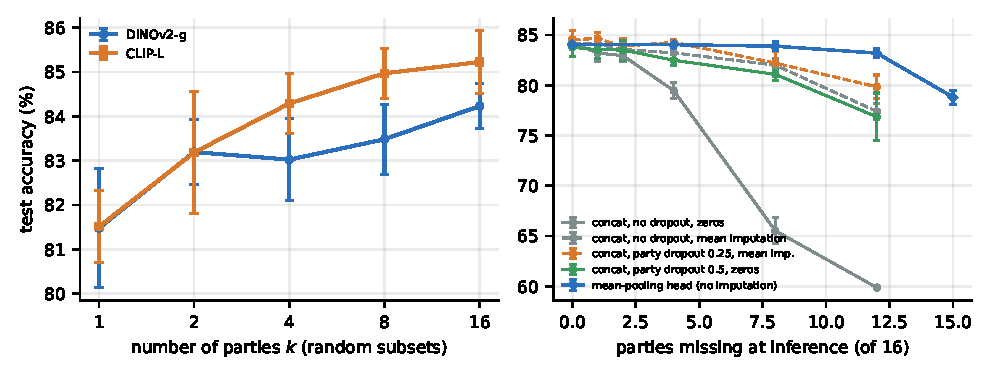
\includegraphics[width=\linewidth]{gen/fig_parties.pdf}
\caption{VertiBench, DINOv2-g. Left: accuracy with $k$ randomly chosen parties (3 subsets $\times$ 5 seeds). Right: parties missing at inference for a concatenation head (missing uploads replaced by zeros or by the party's training mean, with and without party dropout during training) and for a head that averages per-party embeddings.}\label{fig:parties}
\end{figure}

\FloatBarrier

\section{Compression grid}\label{app:pca}

This appendix supports contribution C1: it gives the full grid of local PCA and quantisation from which the main text takes the knee of the frontier, and the limits of compressing without coordination.

\paragraph{Protocol.}
Because the encoder is frozen, each party can fit a PCA on its own training features (keeping $d'\le d$ components; the basis stays with the party) and quantise every coordinate uniformly to $b$ bits between its 1st and 99th training percentiles. The label owner trains the head on the de-quantised values. No labels, shared basis or coordination are needed, but the samples must still be aligned across parties; the few hundred bytes of quantiser bounds that each party sends once are not counted.

\paragraph{Selection under a byte budget.}
On frozen DINOv2-g features we run the grid of Table~\ref{tab:pareto} (16 to 512 components or no PCA, 1 to 16 bits) and select, under each budget, the configuration with the best \emph{validation} accuracy (Fig.~\ref{fig:pareto}). For the 16 parties together, 256\,B per sample (\selTwoCfg) give \selTwoAcc\,\%, 512\,B (\selFiveCfg) \selFiveAcc\,\%, 2\,KiB (\selTwokCfg) \selTwokAcc\,\%, and the full budget selects \selFullCfg{} (\selFullBytes) at \selFullAcc\,\%, against \fullAcc\,\% for the uncompressed 48\,KiB. Moderate compression therefore costs nothing on this benchmark; with 4 bits or more, the PCA-256 and PCA-512 rows are even slightly above the uncompressed features, which we attribute, without having tested it, to a regularising effect on the small labelled set. Even one bit per feature keeps \cmpOneBit\,\%.

\paragraph{Other benchmarks.}
Compression is not free everywhere. On MILK10k a per-party PCA-256 slightly lowers the macro F1 of the concatenation head (\mrGPca, \mrCPca{} and \mrMPca\,\% against \mrGCat, \mrCCat{} and \mrMCat\,\% with DINOv2-g, CLIP-L and MONET; Table~\ref{tab:milkreg}). On WorldStrat, PCA-256 per party changes IPCC and LCCS F1 by \wpIpccPca{} and \wpLccsPca{} points relative to concatenation of the same inputs (Table~\ref{tab:wsfusion}).

\paragraph{Missing parties.}
A concatenation head breaks when parties are missing at inference and their uploads are replaced by zeros (\missZeroEightZ\,\% with 8 of 16 missing, \missZeroTwelveZ\,\% with 12); imputing the party's training mean (\missZeroTwelveM\,\% with 12 missing) or training with party dropout 0.5 (\missHTwelveZ\,\%) repairs most of it (Fig.~\ref{fig:parties}, right). A pooling head (App.~\ref{app:repro}) needs neither: it reaches \poolGMean\,\% with all parties, \poolMissTwelve\,\% with 12 missing and still \poolMissFifteen\,\% with a single party left. It requires a shared feature space, however, and uncoordinated compression removes it: after per-party PCA-64, whose bases differ between parties, the pooling head drops to \poolGPcaMean\,\%, while concatenation of the same uploads keeps \poolGPcaConcat\,\%. Nor does it apply to parties with different modalities or encoders. Local compression and robustness to missing parties must thus be traded off, unless the parties agree on a common basis (e.g.\ one fitted on public images; not tested).

\begin{figure}[tbp]
\centering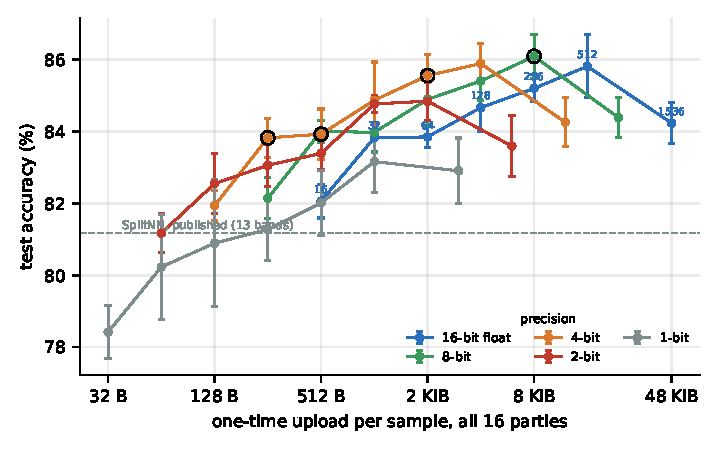
\includegraphics[width=0.78\linewidth]{gen/fig_pareto.pdf}
\caption{VertiBench: accuracy versus one-time upload (bytes per sample, 16 parties) for per-party PCA (number of components annotated on the 16-bit curve) and uniform scalar quantisation of frozen DINOv2-g features, MLP head, 5 seeds. Circles: configuration with the best \emph{validation} accuracy under a budget of 256\,B, 512\,B, 2\,KiB and 48\,KiB.}\label{fig:pareto}
\end{figure}

\begin{table}[tbp]
\caption{The compression grid of Fig.~\ref{fig:pareto} (VertiBench, DINOv2-g, MLP head, 5 seeds). $d'$: PCA components per party (1536: no PCA); $b$: bits per coordinate; upload: one-time payload per sample over the 16 parties. Validation accuracy (seed mean) is the selection criterion; test accuracy and AUC are mean\,$\pm$\,std.}\label{tab:pareto}
\centering\scriptsize
\setlength{\tabcolsep}{4pt}
\begin{tabular}{@{}rrrccc@{}}
\toprule
$d'$ & $b$ & Upload & Val.\ acc.\ (\%) & Test acc.\ (\%) & AUC (\%)\\
\midrule
\inputtab{gen/tab_pareto.tex}
\bottomrule
\end{tabular}
\end{table}

\FloatBarrier

\section{VertiBench audit}\label{app:audit}

This appendix supports contribution C2: it details the audit of the official VertiBench Satellite split and the paired tests behind the comparisons with SplitNN in the main text.

\paragraph{Mapping to source areas.}
Image fingerprints match \auMapTrain{} training and \auMapTest{} test samples to distinct WorldStrat areas (5th-percentile correlation \auScore); \auMapOverlap{} areas appear in both splits.

\paragraph{Siblings, confounded with class.}
The split is not grouped by site, however: \auSibN{} test samples (\auSibShare\,\%) have a training tile from the same site, all from the two sources whose sites are cut into $3\times3$ tiles. They account for \auSibN{} of the 113 test samples in classes 0 and 1, so the \auNoSibN{} test samples without a known sibling are almost all of classes 2 and 3, and class and sibling effects cannot be separated. Table~\ref{tab:audit} gives each head's accuracy on the two subsets. SplitNN is markedly more accurate with siblings (\auSnSib{} vs.\ \auSnNoSib\,\%); the one-shot heads are similarly accurate on both (CLIP-L: \auClipSib{} vs.\ \auClipNoSib\,\%), and the four-logit CLIP heads and frozen split learning are \emph{less} accurate with siblings. The margins over SplitNN are therefore larger on the subset without siblings.

\paragraph{Paired tests.}
The three-seed SplitNN re-run that retains test probabilities averages \auSnAll\,\% accuracy, versus \reproAcc\,\% over five seeds in Table~\ref{tab:main}. We pair test predictions after averaging probabilities over the same three seeds per method (exact McNemar test and 95\,\% paired bootstrap interval, 10{,}000 resamples). On the whole test set, the two CLIP one-shot MLPs, the three four-logit heads and CLIP-B split learning with LoRA beat SplitNN at the 5\,\% level; DINOv2-g's one-shot MLP ($+\pairSnGDiff$ points, $p\pairSnGP$) and frozen CLIP-B split learning do not (Table~\ref{tab:audit}). In detail, the CLIP-L, CLIP-B and DINOv2-g one-shot heads gain $\pairSnClipDiff$ ($p\pairSnClipP$), $\pairSnClipBDiff$ ($p\pairSnClipBP$) and $\pairSnGDiff$ points ($p\pairSnGP$); the CLIP-L, DINOv2-g and CLIP-B four-logit heads give $p\pairSnLgClipP$, $p\pairSnLgGP$ and $p\pairSnLgClipBP$, LoRA split learning $p\pairSnLoraP$ and frozen split learning $p\pairSnSplitFrozenP$. Without known siblings every margin grows and all are significant (CLIP-L: $\pairSnClipNoSibDiff$ points, $p\pairSnClipNoSibP$). These $p$-values are uncorrected: after a Holm correction over the \holmN{} comparisons, \holmSurvive{} remain below 0.05, LoRA split learning and the CLIP-B four-logit head. LoRA itself is unstable across seeds (\seedLoraMin{} to \seedLoraMax\,\%); paired with the ensemble of the one-shot CLIP-B head on the same seeds, its lead is $\pairLoraHeadDiff$ points ($[\pairLoraHeadLo,\pairLoraHeadHi]$, $p\pairLoraHeadP$).

\paragraph{Nearest public image.}
The retrieval attacker of App.~\ref{app:privacy} does not owe its success to siblings: across test uploads, the label of the nearest public training image in CLIP-L space matches in \nnPubAll\,\% of the cases (\nnPubSib\,\% with known siblings, \nnPubNoSib\,\% without), and the neighbour is itself a sibling in just \nnPubIsSib\,\% of the sibling cases, about 5\,\% overall.

\begin{table}[tbp]
\caption{VertiBench audit. Test accuracy (\%) on all 785 test samples, on the \auSibN{} with a training tile from the same site and on the \auNoSibN{} without; paired gain over SplitNN in points with 95\,\% paired bootstrap interval and exact McNemar test, on all samples and without siblings. Probabilities averaged over 3 seeds per method.}\label{tab:audit}
\centering\scriptsize
\setlength{\tabcolsep}{3pt}
\begin{adjustbox}{max width=\linewidth}
\begin{tabular}{@{}lccccccc@{}}
\toprule
& \multicolumn{3}{c}{Accuracy (\%)} & \multicolumn{2}{c}{Gain over SplitNN, all} & \multicolumn{2}{c@{}}{Gain, no sibling}\\
\cmidrule(lr){2-4}\cmidrule(lr){5-6}\cmidrule(l){7-8}
Head & all & sibling & no sibling & points [95\,\% CI] & McNemar & points [95\,\% CI] & McNemar\\
\midrule
SplitNN, VertiBench recipe & \auSnAll & \auSnSib & \auSnNoSib & -- & -- & -- & --\\
\midrule
One-shot MLP, CLIP-L & \auClipAll & \auClipSib & \auClipNoSib & $\pairSnClipDiff$ $[\pairSnClipLo,\pairSnClipHi]$ & $p\pairSnClipP$ & $\pairSnClipNoSibDiff$ $[\pairSnClipNoSibLo,\pairSnClipNoSibHi]$ & $p\pairSnClipNoSibP$\\
One-shot MLP, CLIP-B & \auClipBAll & \auClipBSib & \auClipBNoSib & $\pairSnClipBDiff$ $[\pairSnClipBLo,\pairSnClipBHi]$ & $p\pairSnClipBP$ & $\pairSnClipBNoSibDiff$ $[\pairSnClipBNoSibLo,\pairSnClipBNoSibHi]$ & $p\pairSnClipBNoSibP$\\
One-shot MLP, DINOv2-g & \auGAll & \auGSib & \auGNoSib & $\pairSnGDiff$ $[\pairSnGLo,\pairSnGHi]$ & $p\pairSnGP$ & $\pairSnGNoSibDiff$ $[\pairSnGNoSibLo,\pairSnGNoSibHi]$ & $p\pairSnGNoSibP$\\
\midrule
Four-logit head, CLIP-L & \auLgClipAll & \auLgClipSib & \auLgClipNoSib & $\pairSnLgClipDiff$ $[\pairSnLgClipLo,\pairSnLgClipHi]$ & $p\pairSnLgClipP$ & $\pairSnLgClipNoSibDiff$ $[\pairSnLgClipNoSibLo,\pairSnLgClipNoSibHi]$ & $p\pairSnLgClipNoSibP$\\
Four-logit head, CLIP-B & \auLgClipBAll & \auLgClipBSib & \auLgClipBNoSib & $\pairSnLgClipBDiff$ $[\pairSnLgClipBLo,\pairSnLgClipBHi]$ & $p\pairSnLgClipBP$ & $\pairSnLgClipBNoSibDiff$ $[\pairSnLgClipBNoSibLo,\pairSnLgClipBNoSibHi]$ & $p\pairSnLgClipBNoSibP$\\
Four-logit head, DINOv2-g & \auLgGAll & \auLgGSib & \auLgGNoSib & $\pairSnLgGDiff$ $[\pairSnLgGLo,\pairSnLgGHi]$ & $p\pairSnLgGP$ & $\pairSnLgGNoSibDiff$ $[\pairSnLgGNoSibLo,\pairSnLgGNoSibHi]$ & $p\pairSnLgGNoSibP$\\
\midrule
Split learning, CLIP-B frozen & \auSplitFrozenAll & \auSplitFrozenSib & \auSplitFrozenNoSib & $\pairSnSplitFrozenDiff$ $[\pairSnSplitFrozenLo,\pairSnSplitFrozenHi]$ & $p\pairSnSplitFrozenP$ & $\pairSnSplitFrozenNoSibDiff$ $[\pairSnSplitFrozenNoSibLo,\pairSnSplitFrozenNoSibHi]$ & $p\pairSnSplitFrozenNoSibP$\\
Split learning, CLIP-B LoRA & \auLoraAll & \auLoraSib & \auLoraNoSib & $\pairSnLoraDiff$ $[\pairSnLoraLo,\pairSnLoraHi]$ & $p\pairSnLoraP$ & $\pairSnLoraNoSibDiff$ $[\pairSnLoraNoSibLo,\pairSnLoraNoSibHi]$ & $p\pairSnLoraNoSibP$\\
\bottomrule
\end{tabular}
\end{adjustbox}
\end{table}

\FloatBarrier

\section{MILK10k details}\label{app:milk}

This appendix supports contribution C1: it gives the party combinations, fusion heads and regularisation checks behind the frozen MILK10k rows of Table~\ref{tab:freeze}, and the same-recipe comparison of frozen and adapted backbones. Figure~\ref{fig:frontier-axes-milk} places the MILK10k points on the other axes of the cost accounting: one-shot points need \frMilkRoundsMatch{} message against \frMilkRoundsSplitNN{} for ResNet-18 split learning, and \frMilkGflopsMatchName{} exceeds that baseline (\frMilkGflopsMatchAcc{} vs.\ \frMilkBestNonFound\,\%) with \frMilkGflopsRatio{} times less party compute.

\begin{figure}[t]
\centering\IfFileExists{gen/fig_frontier_axes_milk.pdf}{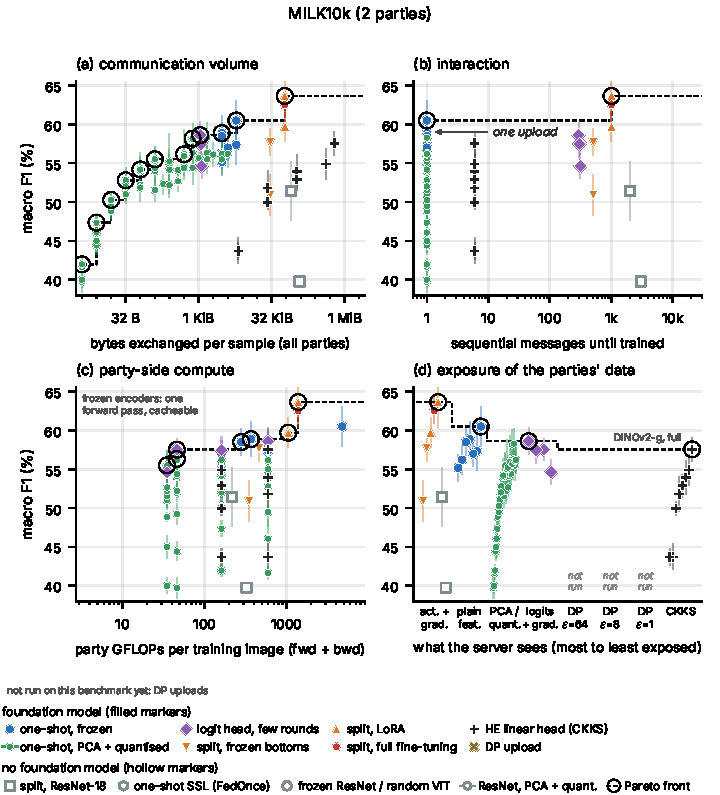
\includegraphics[width=\linewidth]{gen/fig_frontier_axes_milk.pdf}}{\fbox{\parbox{0.9\linewidth}{\centering fig\_frontier\_axes\_milk pending}}}
\caption{MILK10k along the axes of Fig.~\ref{fig:frontier-axes}: (a)~bytes per training sample, (b)~sequential messages until trained, (c)~party GFLOPs per training image (forward and backward), (d)~exposure ladder. Only DP is marked as not run. Circled: Pareto-optimal points.}\label{fig:frontier-axes-milk}
\end{figure}

\begin{table}[tbp]
\caption{MILK10k, all methods (2 parties, 5 folds, class-balanced loss). Split learning trains the bottoms with the server's gradients; one-shot rows use frozen features and an MLP head (concatenation, or late fusion on features averaged over 8 rotations and flips). Upload per training sample: over all training epochs for split learning (30 for ResNet-18 from scratch, 20 from ImageNet, 10 for ViTs), once for one-shot. Time: minutes per fold (one-shot: encoding, estimated).}\label{tab:freeze}
\centering\scriptsize
\setlength{\tabcolsep}{3pt}
\begin{adjustbox}{max width=\linewidth}
\begin{tabular}{@{}llrrrccc@{}}
\toprule
Party models & Training & Trainable & Upload & Time & F1 (\%) & Bal.\ acc.\ (\%) & Acc.\ (\%)\\
\midrule
\inputtab{gen/tab_freeze.tex}
\bottomrule
\end{tabular}
\end{adjustbox}
\end{table}

\paragraph{Real modalities complement each other little.}
The dermoscopic image alone gives \milkGDerm\,\% macro F1 with DINOv2-g, the clinical photograph \milkGClin\,\%, the metadata \milkMeta\,\% (Table~\ref{tab:milk}). Concatenating the two images adds less than one point over the dermoscopy (\milkGBoth\,\%), three points with CLIP-L (\milkCDerm{} $\to$ \milkCBoth\,\%); the metadata add at most one point on top. The general-purpose encoders match or beat the medical ones (BiomedCLIP, MONET). Splitting the dermoscopy into two halves, as split benchmarks do, \emph{loses} information instead: \milkGHalves\,\% against \milkGDerm\,\% for the whole image, because each party's encoder sees half a lesion. Two caveats apply to all MILK10k numbers: folds are drawn over lesions, as the release has no patient identifiers, and each test fold holds only 40 to 61 lesions of the two rarest classes.

\paragraph{How the parties are combined matters as much as the encoder.}
A concatenation MLP under-uses the weaker party. Training one head per party and averaging their log-probabilities (late fusion) is better for every encoder (Table~\ref{tab:milkfusion}): \mfGLate\,\% instead of \mfGCat\,\% with DINOv2-g, \mfCLate\,\% instead of \mfCCat\,\% with CLIP-L, \mfGMLate\,\% when each party uploads DINOv2-g and MONET features; with DINOv2-g, the two parties together then reach \mfGLate\,\%, about three points more than the dermoscopic party alone (\milkGDerm\,\%). Late fusion also suits VFL: each party's head can be trained, audited and dropped independently. The gain is bounded by the data: \mfGBoth\,\% of the lesions are misclassified by both single-party heads, against \mfGIndep\,\% if their errors were independent---the two modalities fail on the same, intrinsically hard lesions.

\paragraph{Over-fitting or modality competition?}
With 3{,}100 training lesions and 2--3k input dimensions, the concatenation head could simply over-fit. Three observations speak against this being the main cause (Table~\ref{tab:milkreg}). First, regularising it---input dropout, Gaussian feature noise, feature mixup, a per-party PCA---gains at most one point and never reaches late fusion. Second, late fusion does not need its tuned weight: a fixed weight of 0.5 does as well (\mrGLateHalf\,\% with DINOv2-g); paired by fold, it beats concatenation by \mrGPairD\,$\pm$\,\mrGPairS{} points with DINOv2-g (\mrGPairW{} folds out of 5), \mrCPairD\,$\pm$\,\mrCPairS{} with CLIP-L (\mrCPairW/5) and \mrMPairD\,$\pm$\,\mrMPairS{} with MONET (\mrMPairW/5). Third, its advantage does not shrink with more data, as over-fitting would predict: it grows from 25\,\% to 100\,\% of the training folds for CLIP-L and MONET. Nor is it an artefact of our early-stopping rule on the unweighted validation loss: when both heads stop on the class-weighted validation loss or on the validation macro F1, late fusion still wins by \mrStopMin{} to \mrStopMax{} points over \mrStopN{} comparisons (DINOv2-g, CLIP-L, DINOv2-B, CLIP-B; stopping on the weighted loss lowers every head by up to \mrWlossDropMax{} points), and weight decay on the concatenation head leaves a gap of \mrWdMin{} to \mrWdMax{} points. The pattern rather matches the \emph{modality competition} documented for jointly trained multimodal networks~\cite{wang2020makes,huang2022modality,peng2022balanced}: a joint head learns the dominant dermoscopy first and stops before exploiting the clinical photograph, whereas separate heads must each use their own modality fully; the validation-tuned late fusion gives the weaker clinical party a weight of 0.3 to 0.5. Augmentation helps in image space, not in feature space: the parties can encode the 8 rotations and flips of each photograph once (8 times the encoding cost) and upload the mean, which raises late fusion to \mrGLateViews\,\% (DINOv2-g), \mrMLateViews\,\% (MONET), \fzViewsB\,\% (DINOv2-B) and \fzViewsCb\,\% (CLIP-B) at no extra communication. With CLIP-L it helps late fusion little (\mrCLateViews\,\%); there the best head is the concatenation trained on one of the 8 uploaded views per epoch (\mrCCatSampled\,\%, at 8 times the upload).

\paragraph{Frozen versus adapted under the same recipe.}
The frozen and adapted rows of Table~\ref{tab:freeze} differ in more than freezing (augmentation, head, standardisation, optimiser and schedule). In a paired re-run we therefore use the same split-learning recipe with frozen and LoRA bottoms. For DINOv2-B this gives \srFrozenB\,\% macro F1 frozen versus \srLoraB\,\% with LoRA (paired gain $\srGapB\pm\srGapSdB$ points, \srWinsB/5 folds); for CLIP-B, \srFrozenCb\,\% versus \srLoraCb\,\% ($\srGapCb\pm\srGapSdCb$ points, \srWinsCb/5 folds). Relative to the one-shot MLPs, freezing under the split recipe shifts F1 by $\srVsHeadB$ and $\srVsHeadCb$ points, respectively, so the larger same-recipe LoRA gain for CLIP-B partly reflects its weaker frozen baseline under that recipe. Adaptation wins on MILK10k under both recipes.

\begin{table}[tbp]
\caption{MILK10k: macro F1 (\%) of one-shot heads on frozen features for every combination of parties (5 folds, class-balanced MLP head). Bottom: the usual practice of splitting one image into a left and a right party.}\label{tab:milk}
\centering\scriptsize
\setlength{\tabcolsep}{3.5pt}
\begin{adjustbox}{max width=\linewidth}
\begin{tabular}{@{}lcccc@{}}
\toprule
Parties & \inputtab{gen/tab_milk_head.tex}\\
\midrule
\inputtab{gen/tab_milk.tex}
\bottomrule
\end{tabular}
\end{adjustbox}
\end{table}

\begin{table}[tbp]
\caption{MILK10k: how the label owner combines the clinical (A) and dermoscopic (B) uploads (macro F1, \%, 5 folds). Late fusion: one head per party, log-probabilities averaged with a weight chosen on the validation fold. Branches: per-party projection, auxiliary per-party losses and modality dropout (0.3). Last column: share of test lesions misclassified by both single-party heads, and (in brackets) what it would be if their errors were independent.}\label{tab:milkfusion}
\centering\scriptsize
\setlength{\tabcolsep}{3pt}
\begin{adjustbox}{max width=\linewidth}
\begin{tabular}{@{}lcccccc@{}}
\toprule
Encoder & B alone & A+B concat & A+B late fusion & A+B branches & A+B+C branches & Both wrong (\%)\\
\midrule
\inputtab{gen/tab_milkfusion.tex}
\bottomrule
\end{tabular}
\end{adjustbox}
\end{table}

\begin{table}[tbp]
\caption{MILK10k, clinical + dermoscopic parties: is the concatenation head over-fitting? Macro F1 (\%, 5 folds). Top: regularising the concatenation head versus late fusion. Middle: augmentation precomputed once by the parties (8 rotations and flips of each photograph). Bottom: gap between late fusion (fixed weight) and concatenation when the training folds are subsampled, and under other early-stopping rules than the unweighted validation loss.}\label{tab:milkreg}
\centering\scriptsize
\setlength{\tabcolsep}{3.5pt}
\begin{adjustbox}{max width=\linewidth}
\begin{tabular}{@{}lccc@{}}
\toprule
Head & DINOv2-g & CLIP-L & MONET\\
\midrule
\inputtab{gen/tab_milkreg.tex}
\bottomrule
\end{tabular}
\end{adjustbox}
\end{table}

\FloatBarrier

\section{WorldStrat: two sensors}\label{app:ws}

This appendix supports contribution C2: it reports a third natural partition, with genuinely different sensors, on which the two parties complement each other little once the folds are grouped by site.

\paragraph{Task.}
From the WorldStrat release~\cite{cornebise2022worldstrat} we build a two-party task on its \wsIpccN{} usable areas of $1.58\times1.58$\,km: party A holds the SPOT 6/7 pan-sharpened image (RGB, 1.5\,m, $1050\times1050$ pixels), party B the 16 Sentinel-2 L1C revisits (13 bands, 10\,m). The label owner holds one of three labels of the release metadata, all read at the centre of the area: the LCCS land-cover class of the 300\,m pixel of a global land-cover map~\cite{esa2017cci} (the 18 classes with at least 40 areas), its coarser IPCC category (7 classes), and the degree of urbanisation of the 1\,km SMOD cell (8 classes, from rural very-low-density to urban centre~\cite{pesaresi2019ghsl}). A label therefore describes only the centre of the image (4\,\% of its area for LCCS and IPCC); the parties also encode centre crops of 336\,m and 1\,km. To vary the information held by A, its image is degraded to 3, 6 and 10\,m before encoding, or cut into 16 full-resolution tiles of 262\,px whose features are averaged. Party B encodes every revisit as three composites (RGB, near- and short-wave infrared) and uploads, per composite, the mean over the 16 revisits or over the 8 least cloudy ones (ranked by a locally computed cloud score), possibly with the temporal standard deviation; for a set head it uploads all 16 vectors. The loss is class-balanced and macro F1 is the metric.

\paragraph{Grouped cross-validation.}
The five folds are stratified and grouped by site: all nine tiles of a site stay in the same fold. Stratification alone split sibling tiles across training and test and gave macro F1 about 6 to 9 points higher on the two land-cover tasks---the same leakage as in the official VertiBench split, which is built from the same areas (App.~\ref{app:audit}). All results below are site-grouped and paired by fold.

\paragraph{The second sensor adds little.}
Alone, the 1.5\,m SPOT image scores \wsIpccSpot{} against \wsIpccSms\,\% macro F1 for the Sentinel-2 revisits (RGB, NIR, SWIR) on IPCC, \wsLccsSpot{} against \wsLccsSms\,\% on LCCS and \wsSmodSpot{} against \wsSmodSms\,\% on SMOD (Table~\ref{tab:ws}). Their concatenation reaches \wsIpccFus, \wsLccsFus{} and \wsSmodFus\,\%: relative to SPOT, F1 changes by \wgIpccA{} points on IPCC (\wgIpccAW{} folds improve), \wgLccsA{} on LCCS (\wgLccsAW) and \wgSmodA{} on SMOD (\wgSmodAW). With DINOv2-g, the pair is thus at most a couple of points above the better single sensor on land cover, and below SPOT alone on urbanisation. The second sensor matters more when the first is weakened (Fig.~\ref{fig:ws}): at 3\,m, fusion adds \wgIpccThree{} points on IPCC (\wgIpccThreeW) and \wgLccsThree{} on LCCS (\wgLccsThreeW); at 10\,m, \wgIpccTen{} (\wgIpccTenW) and \wgLccsTen{} (\wgLccsTenW), whereas SMOD never gains (\wgSmodTen{} at 10\,m, \wgSmodTenW). For land cover, SPOT improves alone at 3\,m (\wsIpccSpotThree{} and \wsLccsSpotThree\,\%) or by averaging the features of 16 full-resolution tiles (\wfIpccSpotTiles{} and \wfLccsSpotTiles\,\%), rather than feeding DINOv2 the whole 1{,}050\,px image; adding the clearest revisits to the tiles yields \wpIpccTilesFus{} and \wpLccsTilesFus{} points (\wpIpccTilesFusW{} and \wpLccsTilesFusW). Adding infrared to RGB helps LCCS at native resolution and both land-cover labels at 10\,m. With a multispectral encoder (SSL4EO-S12 on the 13 bands) for party B, or CLIP-L for both parties, fused IPCC scores and their gain over the single sensors are larger (Table~\ref{tab:ws}), while SMOD barely changes; we did not test these rows in pairs. For native-resolution fusion, pooled out-of-fold per-class F1 gains over SPOT are largest for \wcIpccTop{} on IPCC and \wcLccsTop{} on LCCS (points and number of areas); F1 falls in \wcIpccNeg{} IPCC and \wcLccsNeg{} LCCS classes.

\paragraph{Why a second sensor adds little.}
The parties fail on the same areas: on IPCC both are wrong on \wfIpccBoth\,\% of them, nearly three times the \wfIpccIndep\,\% expected from independent errors, although an oracle choosing the right party would reach \wfIpccOracle\,\% accuracy. Context matters more than a second view of the labelled pixel: although labels are read at the centre of the area, the whole 1.58\,km SPOT image beats a 336\,m centre crop by \wpIpccCentre, \wpLccsCentre{} and \wpSmodCentre{} points (\wpIpccCentreW, \wpLccsCentreW{} and \wpSmodCentreW{} folds); with a 1\,km crop, land-cover scores are roughly unchanged and only SMOD still loses ground (\wfSmodSpotCk{} vs.\ \wfSmodSpot\,\%).

\paragraph{Fusion heads do not change the picture.}
No fusion variant of Table~\ref{tab:wsfusion} improves on plain-mean concatenation across all three labels. The set head over the 16 revisits changes F1 by \wpLccsSetCat{} to \wpIpccSetCat{} points while multiplying the Sentinel-2 payload by 16. Late fusion changes IPCC, LCCS and SMOD F1 by \wpIpccLateMean, \wpLccsLateMean{} and \wpSmodLateMean{} points with the plain mean (SMOD improves in \wpSmodLateMeanW{} folds), and by \wpIpccLateCat, \wpLccsLateCat{} and \wpSmodLateCat{} with the clearest-revisit summary, where the branch head trails concatenation by \wpIpccBranch, \wpLccsBranch{} and \wpSmodBranch{} points. Adding temporal standard deviations shifts the IPCC F1 of Sentinel-2 alone by \wpIpccStdSolo{} points (\wpIpccStdSoloW{} folds improve), and adding a centre crop to SPOT alone changes IPCC and LCCS by \wpIpccFC{} and \wpLccsFC{} points.

\begin{table}[tbp]
\caption{WorldStrat, 5 site-grouped folds: macro F1 (\%, mean\,$\pm$\,std) of each sensor alone and of their concatenation (MLP head; DINOv2-g unless noted). A: SPOT image; B: mean of the 16 Sentinel-2 revisits, encoded as RGB, as three composites (RGB, NIR, SWIR) or on all 13 bands by SSL4EO-S12. Note the column order.}\label{tab:ws}
\centering\scriptsize
\setlength{\tabcolsep}{4pt}
\begin{tabular}{@{}lccc@{}}
\toprule
Parties & IPCC & SMOD & LCCS\\
\midrule
\inputtab{gen/tab_ws.tex}
\bottomrule
\end{tabular}
\end{table}

\begin{figure}[tbp]
\centering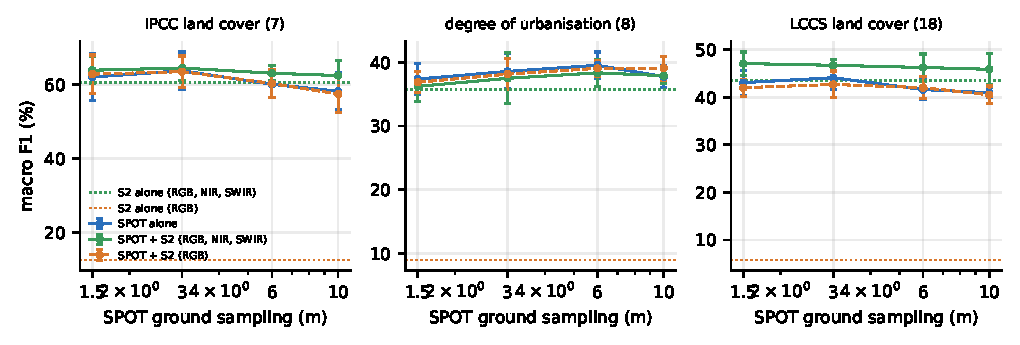
\includegraphics[width=\linewidth]{gen/fig_ws.pdf}
\caption{WorldStrat: macro F1 (mean over 5 site-grouped folds, DINOv2-g, MLP head) of the SPOT party alone and with the Sentinel-2 party, as the SPOT image is degraded from 1.5 to 10\,m. Dotted: Sentinel-2 alone. Fold standard deviations are about 1 to 6 points; paired differences are given in the text.}\label{fig:ws}
\end{figure}

\begin{table}[tbp]
\caption{WorldStrat: single parties and fusion heads (macro F1, \%, mean\,$\pm$\,std over 5 site-grouped folds, DINOv2-g). S2 vectors: number of 4{,}608-d vectors (RGB, NIR and SWIR composites) the Sentinel-2 party uploads per area; the SPOT party uploads one 1{,}536-d vector (two with the centre crop, three with three scales). C: whole SPOT image and mean of the 8 least cloudy revisits. All variants remain one-shot.}\label{tab:wsfusion}
\centering\scriptsize
\setlength{\tabcolsep}{3pt}
\begin{adjustbox}{max width=\linewidth}
\begin{tabular}{@{}lcccc@{}}
\toprule
Configuration & S2 vectors & IPCC & LCCS & SMOD\\
\midrule
\inputtab{gen/tab_wsfusion.tex}
\bottomrule
\end{tabular}
\end{adjustbox}
\end{table}

\FloatBarrier

\section{Classic split benchmarks}\label{app:classic}

This appendix supports contribution C2 by showing why natural benchmarks are needed: on the classic CIFAR and ModelNet40 splits, the gains of a single upload of frozen features mostly measure pre-training.

\paragraph{Splits.}
CIFAR-10/100~\cite{krizhevsky2009cifar} are split as in the papers we compare with: top/bottom halves ($K=2$) and $16\times16$ quadrants ($K=4$) as in VFLAIR~\cite{zou2024vflair} and FedOnce~\cite{wu2022fedonce}, and left/right halves with only $N_o\in\{256,\dots,2048\}$ aligned labelled samples as in Sun et al.~\cite{sun2023oneshotvfl}. Halves are upsampled by 7 ($16\times32\to112\times224$) and quadrants by 14 ($16\times16\to224\times224$), so four quadrants are encoded with four times as many tokens as two halves ($4\times256$ against $2\times128$). ModelNet40~\cite{wu2015modelnet} uses 12 rendered views per object~\cite{su2015mvcnn} (9{,}843 training and 2{,}468 test objects), one view per party ($K=12$) or three per party ($K=4$). We quote the published numbers of the original papers, including VIMADMM~\cite{xie2024vimadmm}.

\paragraph{Large gains that mostly measure pre-training.}
Frozen DINOv2-g features beat every published number by a wide margin (Table~\ref{tab:classic}): \cTenGTwo\,\% on CIFAR-10 cut into top and bottom halves (VFLAIR's split learning: 79.8\,\%), \cTenGFour\,\% with four quadrants (VFLAIR: 76.2\,\%, FedOnce: 58.7\,\%), and \sunA\,\% with only 256 aligned labelled samples, where the semi-supervised three-message protocol of Sun et al.\ reaches 78--80\,\%. On CIFAR-100 the margin is wider still (\cHunGTwo\,\% and \cHunGFour\,\% against 42.3 and 38.2\,\% for VFLAIR), and on ModelNet40 with three views per party DINOv2-g reaches \mnGFour\,\% against 91.3\,\% for VIMADMM and 90.0\,\% for split learning with trained ResNet-18 bottoms. For DINOv2-g, four parties do better than two on CIFAR-100, possibly because the four uploads describe the image with four times as many tokens; we did not test this at an equal token budget, and CLIP-L goes the other way (\cHunCTwo{} to \cHunCFour\,\%). CLIP-L is less robust to small upsampled pieces (\cHunCFour\,\% on CIFAR-100 quadrants against \cHunCCent\,\% on full images), DINOv2-g much more (\cHunGFour{} against \cHunGCent\,\%). These gains should not be over-interpreted: the published baselines train small encoders from scratch, and CIFAR's classes are central to web-scale pre-training data, so a split CIFAR benchmark mostly measures the encoder's pre-training. The splits also create complementarity by construction: one CIFAR-10 quadrant alone gives \cTenGSoloQ\,\%, the four together \cTenGFour\,\%, whereas real parties often see the same object almost completely (App.~\ref{app:milk}). Hence the main text uses naturally partitioned data.

\begin{table}[tbp]
\caption{Classic split benchmarks: one upload of frozen features (224\,px, MLP head, 3 seeds; 5 seeds for the protocol of Sun et al.) against the published numbers of methods that train the party models, under the same splits. CIFAR halves are upsampled to $112\times224$, quadrants to $224\times224$; ModelNet40 uses 12 rendered views. Bottom: left/right CIFAR-10 halves with $N_o$ aligned labelled samples.}\label{tab:classic}
\centering\scriptsize
\setlength{\tabcolsep}{3pt}
\begin{adjustbox}{max width=\linewidth}
\begin{tabular}{@{}llp{4.3cm}cc@{}}
\toprule
Data & Split & Published (acc.\,\%) & DINOv2-g & CLIP-L\\
\midrule
\inputtab{gen/tab_classic.tex}
\bottomrule
\end{tabular}
\end{adjustbox}

\vspace{4pt}
\begin{adjustbox}{max width=\linewidth}
\begin{tabular}{@{}rcccc@{}}
\toprule
Aligned samples $N_o$ & Sun et al.\ one-shot & Sun et al.\ few-shot & DINOv2-g & CLIP-L\\
\midrule
\inputtab{gen/tab_sun.tex}
\bottomrule
\end{tabular}
\end{adjustbox}
\end{table}

\FloatBarrier

\section{Privacy details}\label{app:privacy}

This appendix supports contribution C1: it details the attacks on plaintext uploads, the party-side transforms, the differential-privacy mechanism and the parameters and cost of encrypted training that place the regimes on the exposure axis.

\subsection{Attacks on plaintext uploads}

\paragraph{Linkage.}
An attacker holding public copies of the candidate images needs no decoder: encoding them with the public encoder and matching the uploads links each upload to its image. Exact re-encoding links \giLink\,\% of the uploads within one party. Across the full gallery of the \lkN{} test images of the 16 parties, top-1 linkage rounds to \lkSame\,\% with identical preprocessing (\lkDup{} uploads have duplicates), versus \lkBicubic\,\% after bicubic resizing, \lkEightbit\,\% after 8-bit quantisation of the resized image and \lkClip\,\% with CLIP's standard preprocessing of the same encoder; within a single party, even the worst party still links \lkClipParty\,\% under that last mismatch.

\paragraph{Generic decoder.}
The encoders are public, so the attacker does not need in-domain pairs either: for OpenAI CLIP ViT-L/14, Stable unCLIP~2.1 (``small'')~\cite{ramesh2022unclip,rombach2022ldm} generates an image from the CLIP image embedding, which is the pooled output a party uploads times the public projection matrix of the encoder. We decode, without any adaptation, the CLIP-L uploads of \giVbN{} VertiBench test images of one party and of \giMilkN{} MILK10k test lesions per modality (25 denoising steps, guidance scale~10, empty text prompt). Pixel metrics say little about a generator that does not reproduce brightness or exact layout, so we measure what the attacker learns with an independent encoder, DINOv2 ViT-B/14: re-identification of the source among all candidates (the \giVbNTest{} test images of the party, all \giMilkNGal{} MILK10k lesions) by the cosine of DINOv2-B features (VertiBench images contrast-stretched per channel), and the label predicted from the reconstruction by a logistic regression trained on the DINOv2-B features of real training images. On VertiBench (Fig.~\ref{fig:generic}) the pixels are lost (PSNR \giVbPsnr\,dB; a reconstruction is closer to its source than to any other test image in \giVbPixReid\,\% of the cases), yet the independent encoder picks the source in \giVbReid\,\% of the cases (top-10: \giVbReidTen\,\%; chance: \giVbChance{} and \giVbChanceTen\,\%), and the label of the reconstruction is predicted with \giVbLabFone\,\% macro F1, against \giVbRealFone\,\% from the image itself and \giVbChanceFone\,\% from the class frequencies. A party that encodes its images with CLIP's own preprocessing rather than ours leaks as much (\giVbClipReid\,\% and \giVbClipLabFone\,\%). On MILK10k the decoder draws skin with a lesion-like spot, but recovers neither the lesion (top-10 re-identification: \giMilkClinReidTen\,\% clinical, \giMilkDermReidTen\,\% dermoscopic) nor its diagnosis (\giMilkClinLabFone{} and \giMilkDermLabFone\,\% macro F1; chance \giMilkChanceFone, real images \giMilkClinRealFone{} and \giMilkDermRealFone\,\%): what a generic decoder recovers depends on how well its training images cover the domain. For the pooled DINOv2 token we found no public decoder---decoders from DINOv2 \emph{patch} tokens~\cite{zheng2026rae} and diffusion-guided attacks on intermediate features~\cite{lei2025drag} exist---so we did not attack DINOv2 uploads this way; it is feasible in principle, by training such a decoder once on public images~\cite{bordes2022rcdm} or by mapping DINOv2 to CLIP embeddings with public images.

\paragraph{Fine-tuned decoder and retrieval.}
On VertiBench we also give the decoder the attacker's best chance: we fine-tune all the weights of its denoising network on public in-domain pairs---the RGB composites of the 16 revisits of \giftLocs{} training locations, standing for public Sentinel-2 images (brightened 1.6 times, at $\giftSize\times\giftSize$ pixels), with their CLIP-L embeddings: \giftPairs{} pairs---with its usual v-prediction loss, for \giftMinutes{} minutes on one GPU (\giftSteps{} steps of 32 pairs, learning rate $10^{-5}$, embedding dropped for 10\,\% of the pairs so that classifier-free guidance still works). Its guidance scale (among \giftGuidGrid) is chosen on 200 other training locations by the cosine between the CLIP-L embeddings of the decoded image and of the source, and the attacker keeps the best of \giftNBest{} samples per upload, the one whose embedding is closest to the upload. The fine-tuned decoder draws Sentinel-2-like composites (Fig.~\ref{fig:generic-ft}) whose CLIP embedding is closer to the upload (cosine \giftBestClip, against \giftOffClip{} for the off-the-shelf decoder at the same \giftSize-pixel resolution, where it fails: \giVbOffLabFone\,\% macro F1) and whose pixels are closer to the source (PSNR \giVbBestPsnr\,dB), as it has learnt their brightness and colours; but it re-identifies the source no more often (\giVbBestReid\,\%, top-10 \giVbBestReidTen\,\%) and predicts its label only slightly better (\giVbBestLabFone\,\% macro F1). The same public pairs give a \emph{retrieval} attacker, which returns the public image whose CLIP-L embedding is nearest to the upload: it is matched back to the source in \giVbNnReid\,\% of the cases by the independent encoder (top-10: \giVbNnReidTen\,\%) and predicts the label with \giVbNnLabFone\,\% macro F1, as well as the real image does; App.~\ref{app:audit} shows that this does not rest on siblings.

\paragraph{Decoders trained on in-domain pairs.}
A curious label owner holding auxiliary image--feature pairs from the same distribution (cheap when the imagery and the encoder are public) can also train decoders from one uploaded vector to the $64\times64$ RGB thumbnail of its party: a deconvolutional network with a pixel-wise MSE loss over the 50k training pairs, trained for \invEpochs{} epochs (AdamW, one-cycle schedule) and shared by all parties, or for \invShortEpochs{} epochs (Adam) with a learned per-party affine input map initialised at the identity (the long variant uses such a map only for per-party PCA, whose bases differ); and a closed-form linear (ridge) decoder, fitted per party for PCA uploads. For compressed uploads the attacker knows the party's PCA basis; for randomised uploads it draws fresh noise at every training step. We report PSNR, SSIM~\cite{wang2004ssim} and two re-identification rates on $16\times16$ thumbnails (source image among the test images; source location among the \invNLoc{} test locations, at any date), calibrated by the mean training image, each image's own mean colour and the nearest training image in feature space. From one full upload, the decoder reaches \invFull\,dB PSNR (Table~\ref{tab:privacy}, Fig.~\ref{fig:inversion}): better than the mean training image (\invMean\,dB) or the nearest training image in feature space (\invNN\,dB), but \emph{worse} than painting each image with its own mean colour (\invColour\,dB); the linear decoder reaches \invLinFull\,dB. The decoder is not under-trained: on its training images its error (MSE \invFullTrainMse) is less than a quarter of that of the mean-colour rendering (\invColourTrainMse), but this does not carry over to unseen images, and training it for \invEpochs{} rather than \invShortEpochs{} epochs gains only \invGainLong\,dB. Reconstructions single out their source among the \lkN{} test images in \invFullReid\,\% of the cases and its location in \invFullReidLoc\,\% (top-10: \invFullReidLocTen\,\%; chance: 0.01, \invChanceLoc{} and \invChanceLocTen\,\%), less often than the mean-colour rendering (\invColourReidLoc{} and \invColourReidLocTen\,\%). Compression lowers this leakage at little cost in accuracy: after PCA-16 the best attacker reaches \invBestPCAst\,dB and finds the location in \invBestPCAstReidLoc\,\% of the cases. A pixel-loss decoder is a weak attacker; these numbers bound the leakage from below.

\subsection{Party-side transforms}

A party can transform its features before uploading them, at no communication cost: a secret random rotation; its own PCA-64 basis; the 100-dimensional code of an autoencoder (MLP, MSE loss) or of a noise-as-targets encoder~\cite{bojanowski2017nat} trained on its own features; or, giving up one-shot training, a linear layer to 100 dimensions trained jointly with the head by split learning. The generic decoder needs CLIP embeddings, so the attacker first learns a map back from the transformed upload. Without any image--upload pair of the party, it matches the eigenvectors of the party's uploads with those of public in-domain features (here the CLIP-L features of the other revisits), in order of eigenvalue and with signs set by the skewness of the projections, which undoes any orthogonal transform up to the ambiguity of close eigenvalues. With $k$ leaked pairs it fits a ridge regression from uploads to CLIP embeddings (or an MLP when $k\ge1{,}000$, if better on held-out pairs).

The rotation costs nothing (\gdRotAcc\,\% accuracy against \gdPlainAcc\,\%), the autoencoder code \gdAeDrop{} points, the private PCA-64 \gdPcaDrop{} and the split-learning bottleneck \gdSplitDrop{} (Table~\ref{tab:defences}). Without leaked pairs, our spectral alignment does not undo them: the embeddings it recovers are further from the true ones (cosine \gdRotCosZero) than the mean embedding is (\giCosMean), and link \gdRotLinkZero\,\% of the uploads; unsupervised alignment methods developed for word embeddings~\cite{conneau2018word,grave2019wasserstein} may do better. With 100 leaked pairs (3\,\% of a party's samples), however, a ridge regression maps the rotation, the PCA and the autoencoder code back to CLIP embeddings that link \gdPcaLinkOneZeroZero{} to \gdAeLinkOneZeroZero\,\% of the uploads (split learning: \gdSplitLinkOneZeroZero\,\%), and 1{,}000 pairs bring all four to at least \gdSplitLinkOneZeroZeroZero\,\% (cosine \gdSplitCosOneZeroZeroZero{} to \gdRotCosOneZeroZeroZero). Only noise as targets resists, with \gdNatLinkThreeOneFourTwo\,\% after all 3{,}142 training pairs, because its codes discard much of the information: they cost \gdNatDrop{} points of accuracy. A transform that preserves accuracy preserves what the attacker needs, and keeping image--upload pairs secret is a weak assumption.

\subsection{Differential privacy of the upload}

Party $k$ clips each vector (raw or after PCA) at the median $\ell_2$ norm $c_k$ of its own training vectors and adds noise $\mathcal{N}(0,\sigma_k^2 I)$. For fixed preprocessing and $c_k$, replacing one record changes the clipped vector by at most $2c_k$, so each release is $\mu$-Gaussian-DP with $\mu=2c_k/\sigma_k$~\cite{dong2022gdp}; we set $\sigma_k$ from a target per-upload $(\varepsilon,\delta=10^{-5})$. The 16 uploads of a sample compose to $4\mu$: a per-upload $\varepsilon=8$ gives $\varepsilon\approx50$ for the sample, and $\varepsilon=64$ gives $\varepsilon\approx630$. These budgets do not account for estimating the clipping norms or fitting the PCA on the training data: the guarantee is formal but loose. Because the clipped signal has a fixed norm while the noise norm grows with the square root of the dimension, PCA is what makes DP usable. On VertiBench with DINOv2-g, a per-upload $\varepsilon=8$ drops the full features to \dpFullEight\,\%, below the \majVB\,\% of always predicting the majority class (the inversion PSNR is then that of the mean training image to the reported precision, and re-identification is near chance; Table~\ref{tab:privacy}), whereas after PCA-16 the same budget keeps \dpStEight\,\%, above it. At $\varepsilon=64$, full features give \dpFullSsf\,\%, PCA-64 \dpSfSsf\,\% and PCA-16 \dpStSsf\,\% (PCA-64 at $\varepsilon=8$: \dpSfEight\,\%). PCA followed by DP is thus the privacy end of the frontier: a formal, loose guarantee at an accuracy cost, whereas the reproduced SplitNN, at \reproAcc\,\%, offers no formal guarantee.

\subsection{Encrypted training of a linear head}

\begin{table}[tbp]
\caption{Heads that can be trained on encrypted uploads: accuracy (VertiBench, CIFAR) or macro F1 (MILK10k, WorldStrat), mean\,$\pm$\,std over 5 seeds or folds (CIFAR: 3 seeds). MLP: reference head re-run in the ridge pipeline (hence tenths of a point from Table~\ref{tab:main}). Ridge: closed form on standardised features (class-weighted on MILK10k and WorldStrat), emulated in plaintext, after a per-party PCA to 256, 64 or 16 components; --: too large to emulate.}\label{tab:he}
\centering\scriptsize
\setlength{\tabcolsep}{4pt}
\begin{adjustbox}{max width=\linewidth}
\begin{tabular}{@{}lccccc@{}}
\toprule
& \multicolumn{2}{c}{Full features} & \multicolumn{3}{c}{Ridge after per-party PCA}\\
\cmidrule(lr){2-3}\cmidrule(lr){4-6}
Task & MLP & Ridge & 256 & 64 & 16\\
\midrule
\inputtab{gen/tab_he.tex}
\bottomrule
\end{tabular}
\end{adjustbox}
\end{table}

\paragraph{Protocol.}
After a local PCA to $d'$ components and standardisation, the ridge classifier $W=(X^\top X+\lambda I)^{-1}X^\top Y$ on one-hot targets only needs $X^\top X$ and $X^\top Y$. Every party encrypts its feature columns once with CKKS under a threshold key generated jointly by the parties~\cite{mouchet2021multiparty} (a single key shared by the passive parties would let each of them decrypt the others' uploads); the label owner computes the cross-party blocks $X_k^\top X_l$ and $X_k^\top Y$ homomorphically (multiplicative depth one), masks them with random matrices, has them decrypted and solves the system in the clear: one upload plus one round trip of $\mathcal{O}(D^2)$ aggregates, $D=Kd'$, and no per-sample feature is ever decrypted. With class weights, which depend on the labels, the label owner also sends the encrypted per-sample weights; every party multiplies its columns by them, uploads these weighted columns as well and computes its own weighted Gram block with ciphertext--plaintext products (depth two). The regularisation $\lambda$ is chosen on validation predictions, which the label owner obtains by applying each candidate model to the encrypted validation uploads and decrypting only the scores. The protocol reveals the second-order statistics of the features to the label owner, as the closed-form protocols of~\cite{gascon2017privacy,huang2026vafl}, and does not protect the trained model or its predictions. An encrypted logistic regression (a fixed number of full-batch Nesterov steps with the degree-3 polynomial sigmoid of~\cite{kim2018logistic}) would reveal only the model but needs bootstrapping or a refresh of the encrypted weights every few iterations~\cite{kim2018logistic,han2019logistic}; its accuracy depends on that budget and is not reported. We emulate the ridge in plaintext (CKKS adds relative errors of the order of $10^{-6}$) and time its homomorphic operations with a single key; the interactive key generation and collective decryption of threshold CKKS are not timed.

\paragraph{Accuracy.}
With two parties and full features, the closed-form ridge loses at most 2.1 points relative to the MLP (Table~\ref{tab:he}): it is within 0.2 points on CIFAR-10 and MILK10k with DINOv2-g, loses 1.4 on CIFAR-100 and 2.1 on MILK10k with CLIP-L, and gains 1.4 on WorldStrat IPCC (\heworldstratipccRidgeFull{} versus \heworldstratipccMlp\,\% F1). Reducing the dimension costs accuracy: on VertiBench (16 parties), ridge after a per-party PCA-256 loses 1.6 points with DINOv2-g (\heVbGRidgeTf{} against \heVbGMlp\,\%) and 1.7 with CLIP-L, while PCA-64 loses 2.5 to 7 points relative to the full-feature MLP on the two-party tasks other than CIFAR-100, where it loses about 20. This is not an artefact of standardising each coordinate before the ridge, which inflates the weak PCA components: standardising each party's block as a whole instead, with the choice made on validation, changes the ridge by at most \heSelMax{} points over \heSelN{} configurations. On CIFAR-100 the collapse comes from the squared loss of the ridge with 100 classes rather than from linearity: a linear softmax head on the same PCA-64 features reaches \heCHundredSfLin\,\% (MLP: \heCHundredSfMlp\,\%), but it has no closed form to compute under encryption.

\paragraph{Cost.}
We timed the CKKS operations with TenSEAL (ring degree 8192, one ciphertext per feature column holding up to 4{,}096 training samples, one CPU core): an encrypted inner product of two columns takes about \hcVbStCtCt\,ms, and the label owner needs one per pair of columns from different parties. This amounts to \hcVbStServerH{} core-hours for VertiBench with PCA-16 and \hcVbSfServerH{} with PCA-64; for the class-weighted ridge of MILK10k, whose parties must also compute their own weighted Gram blocks under encryption, \hcMilkServer{} core-minutes with PCA-64, but about \hcMilkFullH{} core-hours (\hcMilkFullUnwH{} without class weights) with the 1{,}536 features per party that the accuracy of the full ridge requires---embarrassingly parallel, but not cheap. Encryption expands each upload $\times$\hcVbSfExpand: with PCA-64, a VertiBench party sends \hcVbSfUp{} for its \hcVbSfN{} training samples instead of \hcVbSfPlain{} in half precision, and a MILK10k party with full features \hcMilkFullUp{} (its columns and their weighted copies). The decryption round trip also needs the encrypted inner products to be repacked into few ciphertexts, which we did not implement. By this estimate, encrypted one-shot VFL with a linear head is affordable with a few dozen features per party, or with full features at about a hundred core-hours for two parties. These are operation timings with a single key, not a measured protocol: the end-to-end time, the collective decryption and the effect of the encoding precision on the predictions remain to be established.

\begin{figure}[tbp]
\centering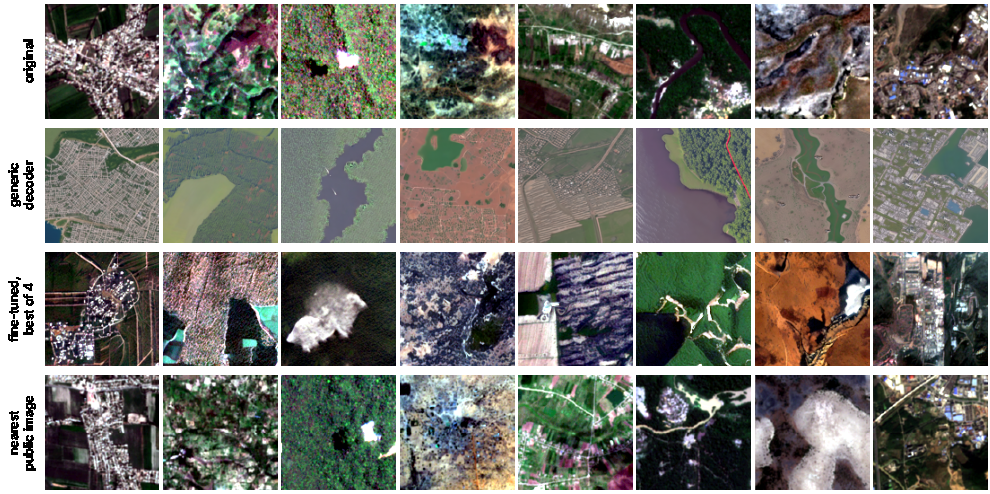
\includegraphics[width=\linewidth]{gen/fig_generic_ft.pdf}
\caption{The first eight attacked VertiBench test images (contrast-stretched for display, as the two bottom rows), the output of the generic decoder of Fig.~\ref{fig:generic}, the best of \giftNBest{} samples of the same decoder fine-tuned on public in-domain pairs, and the public image nearest to the upload in CLIP-L space, which is always of a training location.}\label{fig:generic-ft}
\end{figure}

\begin{figure}[tbp]
\centering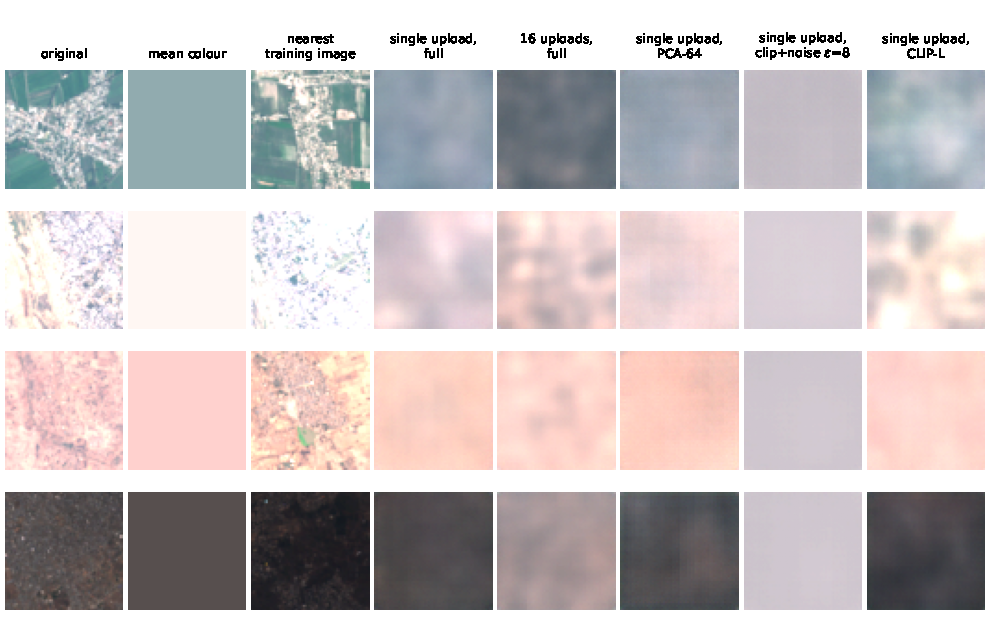
\includegraphics[width=\linewidth]{gen/fig_inversion.pdf}
\caption{Decoders trained on in-domain image--feature pairs, on held-out VertiBench test images ($64\times64$ RGB thumbnails, brightness $\times3$ for display). From left to right: original; its mean colour; nearest training image in DINOv2-g feature space; decoder output from one full DINOv2-g upload, from a PCA-64 upload, from a clipped noisy upload, and from one CLIP-L upload.}\label{fig:inversion}
\end{figure}

\begin{table}[tbp]
\caption{Utility versus leakage of the upload format on VertiBench (DINOv2-g, 224\,px). Accuracy on the test set (5 seeds); PSNR and SSIM of the single-upload inversion; re-identification (top-1, $16\times16$ thumbnails) of the source among the 12{,}560 test images and of its location among the \invNLoc{} test locations. Each value is that of the strongest attacker: the deconvolutional decoder trained for \invEpochs{} epochs, the same trained for \invShortEpochs{} epochs ($^{s}$) or the linear decoder ($^{\ell}$). Clip + noise: per-party Gaussian mechanism, per-upload $(\varepsilon, 10^{-5})$.}\label{tab:privacy}
\centering\scriptsize
\setlength{\tabcolsep}{3.5pt}
\begin{adjustbox}{max width=\linewidth}
\begin{tabular}{@{}lrccccc@{}}
\toprule
 & & & & & \multicolumn{2}{c@{}}{Re-id (\%)}\\\cmidrule(l){6-7}
Upload format & Upload & Acc. (\%) & PSNR (dB) & SSIM & image & location\\
\midrule
\inputtab{gen/tab_privacy.tex}
\bottomrule
\end{tabular}
\end{adjustbox}
\end{table}

\begin{table}[tbp]
\caption{Party-side transforms of the CLIP-L upload on VertiBench. Accuracy of the usual head on the 16 transformed uploads (3 seeds). Linkage: share of the \giVbNTest{} test uploads of a party whose embedding, mapped back to CLIP space from $k$ leaked image--upload pairs of that party ($k=0$: spectral alignment with public in-domain features), is closer to the true CLIP embedding of its image than to that of any other test image (chance \giVbChance\,\%). Raw uploads need no map: the public projection gives the embedding itself.}\label{tab:defences}
\centering\scriptsize
\setlength{\tabcolsep}{4pt}
\begin{tabular}{@{}lrcccccc@{}}
\toprule
& & & \multicolumn{5}{c@{}}{Linkage (\%) with $k$ leaked pairs}\\\cmidrule(l){4-8}
Transform & Dim. & Acc. (\%) & 0 & 10 & 100 & 1{,}000 & 3{,}142\\
\midrule
\inputtab{gen/tab_defences.tex}
\bottomrule
\end{tabular}
\end{table}

\FloatBarrier

\section{Reproducibility}\label{app:repro}

This appendix lists the code, data, compute and training details behind every result of the paper.

\paragraph{Code, data and compute.}
All code, configurations, raw result files and the scripts that generate every table, figure and quoted number from them are in the accompanying repository\footnote{\url{https://github.com/xavierxav/Simple-VFL}, directories \texttt{paper\_experiments} and \texttt{paper\_results}.}. All data sets are public. Each frozen head trains in seconds to minutes on one GPU; the whole study, including the end-to-end baselines, the image augmentation and the WorldStrat feature extraction, used about 110 Google Colab compute units on L4 and A100 GPUs.

\paragraph{Encoders and features.}
All encoders are used through their pooled output token at their native 224\,px input: DINOv2 ViT-S/B/L/g~\cite{oquab2024dinov2}, CLIP ViT-B/16 and ViT-L/14~\cite{radford2021clip}, SigLIP ViT-B/16~\cite{zhai2023siglip}, a supervised ImageNet ResNet-50 and a randomly initialised ViT-B; SSL4EO-S12 ViT-S/16~\cite{wang2023ssl4eo} on all 13 Sentinel-2 bands; BiomedCLIP~\cite{zhang2023biomedclip} and MONET~\cite{kim2024monet} for MILK10k. Satellite images are standardised per band with statistics of the released data (on WorldStrat, estimated on 200 random areas of all folds, without labels) and fed as RGB or as false-colour composites (B8-B4-B3, B12-B8A-B4) to expose the infrared bands to RGB encoders; the SPOT image is encoded at its own pixel count (1050, 518, 266 and 168\,px for 1.5, 3, 6 and 10\,m). Natural images use each model's own normalisation. Features are extracted once in half precision; a party holding several images of an entity (revisits, views) averages their features.

\paragraph{Heads.}
The reference head is a two-layer MLP ($Kd\to1000\to C$, batch normalisation, ReLU; 24.6\,M weights for 16 DINOv2-g parties, 3.1\,M for two). \emph{Late fusion} trains one MLP per party and averages their log-probabilities with a weight $w$ (chosen on the validation fold, or fixed to $\tfrac12$). A \emph{branch} head projects each party to 512 dimensions (linear, LayerNorm, GELU), classifies their concatenation, adds one auxiliary classifier per party (loss weight $\tfrac12$) and, with modality dropout, zeroes one random party in 30\,\% of the training samples. A \emph{pooling} head normalises each party's vector (LayerNorm), averages them over the parties present and applies the MLP; it requires all parties to share an encoder and feature space. A \emph{set} head applies one weight-shared MLP to each of the vectors of a party that holds several images and pools them by attention before the classifier. All heads on frozen features use Adam (learning rate $10^{-3}$, batch 512), at most 50 epochs, \texttt{ReduceLROnPlateau} and early stopping on the unweighted validation loss; the best validation checkpoint is tested (Table~\ref{tab:milkreg} checks two other stopping rules). On the imbalanced WorldStrat and MILK10k labels the loss is class-balanced and macro F1 is the primary metric.

\paragraph{Seeds, folds and tests.}
On VertiBench the public split is used as is (3{,}142 training and 785 test samples); 15\,\% of the training samples are held out for validation with the seed, so seeds change the initialisation and the validation subset, not the test set. We report mean\,$\pm$\,sample standard deviation over five seeds (VertiBench, unless noted), three seeds (CIFAR, ModelNet40; five for the protocol of Sun et al.) or five stratified cross-validation folds (WorldStrat, grouped by site; MILK10k, over lesions), where fold $f$ is the test set and fold $f{+}1$ the validation set. On the fixed VertiBench test set, comparisons use paired bootstrap intervals and exact McNemar tests on test predictions from seed-averaged probabilities (App.~\ref{app:audit}); WorldStrat and MILK10k comparisons are paired by fold. On MILK10k, the age imputation and standardisation of the metadata party are computed on all lesions, without labels.

\paragraph{Baselines.}
\emph{VertiBench recipe}: our re-implementation of the published SplitNN configuration (one ResNet-18 per party with a $9\times9$ stride-2 input convolution, MLP aggregation, Adam with learning rate $10^{-5}$, step decay, batch 32, 50 epochs, last epoch tested, 16 bottoms run sequentially) on the 13 bands. \emph{SplitNN, our recipe}: standard ResNet-18 bottoms~\cite{he2016resnet}, from scratch or ImageNet weights, and the same MLP top model as our head (Adam, one-cycle schedule, 40 epochs, batch 64, flips, best validation checkpoint). \emph{FedOnce}~\cite{wu2022fedonce}: every party trains a ResNet-18 on its unlabelled training images with Noise As Targets~\cite{bojanowski2017nat} (64-d targets, Hungarian re-assignment every 3 epochs, 100 epochs) or SimCLR~\cite{chen2020simclr} and uploads its output once; each party's encoder is pre-trained once and the five seeds re-train the head only, so the standard deviation of these rows is conditional on that pre-training. \emph{Same-backbone split learning}: frozen and LoRA-adapted CLIP ViT-B/16 bottoms on VertiBench; frozen, LoRA-adapted and (for DINOv2) fully fine-tuned CLIP ViT-B/16 and DINOv2 ViT-B/14 bottoms on MILK10k, with ResNet-18 baselines from scratch and from ImageNet weights. LoRA~\cite{hu2022lora} uses rank 16 on the attention query and value projections; the ViT runs use 10 epochs, augmentation and the best validation checkpoint, with a class-balanced loss on MILK10k. These baselines follow published or standard recipes without extensive hyper-parameter search.
.
% Every number is a macro of gen/macros.tex or a value quoted from the published papers.

\section{Full VertiBench results and encoders}\label{app:vb}

This appendix supports both contributions: it details the VertiBench baselines and the comparison of frozen encoders behind the foundation-model points of the frontier (C1), and shows how accuracy depends on the number of parties of this benchmark (C2).

\begin{table}[tbp]
\caption{VertiBench Satellite, all methods (16 parties, official test set). Upload: training payload per sample over all parties (activations or logits up, gradients down when needed). GFLOPs: party compute per image (a training run for split learning, one forward pass otherwise). Time: minutes on one A100 (split training, FedOnce pre-training or feature extraction). Mean\,$\pm$\,std over 5 seeds unless noted; --: not recorded.}\label{tab:main}
\centering\scriptsize
\setlength{\tabcolsep}{3pt}
\begin{adjustbox}{max width=\linewidth}
\begin{tabular}{@{}lcrrrccc@{}}
\toprule
Method & Bands & Upload & GFLOPs & Time & Acc. (\%) & F1 (\%) & AUC (\%)\\
\midrule
\inputtab{gen/tab_main.tex}
\bottomrule
\end{tabular}
\end{adjustbox}
\end{table}

\paragraph{Baselines.}
Our re-implementation of the published VertiBench split-learning configuration reaches $\reproAcc\pm\reproStd$\,\% on the 13 bands after its last epoch, in line with the published $81.2\pm0.4$\,\% (Table~\ref{tab:main}). Our own split-learning recipe is weaker from scratch (\splitAllAcc\,\% on 13 bands, \splitRGBAcc\,\% on RGB) and matches it from ImageNet weights (\splitPTAcc\,\% on RGB). FedOnce, whose parties learn their encoder on their own unlabelled images before a single upload, reaches \natAcc\,\% with Noise As Targets and \sslAllAcc\,\% with SimCLR: on 3{,}142 training locations, self-supervised training does not produce better features than supervised split learning. Macro F1 and AUC order the frozen foundation encoders above these baselines as accuracy does, but not among themselves (CLIP-B has the best macro F1 and a lower accuracy than CLIP-L). No difference between the two best encoders is detected: on the same test predictions (seed-averaged probabilities), CLIP-L leads DINOv2-g by $\pairDiff$ points, 95\,\% bootstrap interval $[\pairLo, \pairHi]$, McNemar $p=\pairP$.

\paragraph{Encoder choice.}
Table~\ref{tab:encoders} compares nine frozen encoders under the same head. All pre-trained ViTs lie between 81.6 and 85.2\,\%, a supervised ImageNet ResNet-50 reaches 80.9\,\%, and a randomly initialised ViT-B only 75.1\,\%: the gain comes from pre-training, not from the head. Size matters moderately: DINOv2 gains 2.4 points from ViT-S/14 (81.8\,\%) to ViT-g/14 (84.2\,\%), whereas CLIP ViT-B/16 is within one point of ViT-L/14. In FLOPs a large encoder is not cheaper than training a small bottom model: one DINOv2-g pass costs \vbGGF{} GFLOPs per image, more than the \rEighteenTrainGF{} GFLOPs of 50 training epochs of the VertiBench ResNet-18 bottom, whereas CLIP-B costs \vbClipBGF{} GFLOPs; encoding all images of the 16 parties takes \vbGMin{} minutes with DINOv2-g and \vbClipBMin{} with CLIP-B on one A100. Parties may also upload the features of two encoders side by side: CLIP-L with CLIP-B reaches \comboLB\,\%, DINOv2-g with CLIP-L \comboGL\,\%, a small gain for a larger upload. The encoder is therefore a parameter of the regime, chosen for cost.

\paragraph{Number of parties.}
The 16 VertiBench parties observe the same sensor at different dates and are largely redundant: with DINOv2-g, one party alone gives \soloMean\,\% on average (\soloMin--\soloMax), two parties \partiesKTwo\,\%, four \partiesKFour\,\%, eight \partiesKEight\,\% and all 16 \partiesKAll\,\% (Fig.~\ref{fig:parties}, left). This redundancy is a property of the benchmark: it limits what any method can gain by combining parties here, and it lets a suitable head tolerate missing parties (App.~\ref{app:pca}).

\begin{table}[tbp]
\caption{Frozen encoders on VertiBench (224\,px RGB, one upload, 5 seeds). Params in millions, GFLOPs per image, $d$ per party. Bottom: each party uploads two encoders' features side by side (features standardised).}\label{tab:encoders}
\centering\scriptsize
\setlength{\tabcolsep}{3.5pt}
\begin{adjustbox}{max width=\linewidth}
\begin{tabular}{@{}lrrrccc@{}}
\toprule
Encoder & Params & GFLOPs & $d$ & Acc. (\%) & F1 (\%) & Linear acc. (\%)\\
\midrule
\inputtab{gen/tab_encoders.tex}
\midrule
\multicolumn{7}{@{}l}{\emph{Each party uploads two encoders' features (standardised)}}\\
\inputtab{gen/tab_combo_enc.tex}
\bottomrule
\end{tabular}
\end{adjustbox}
\end{table}

\begin{figure}[tbp]
\centering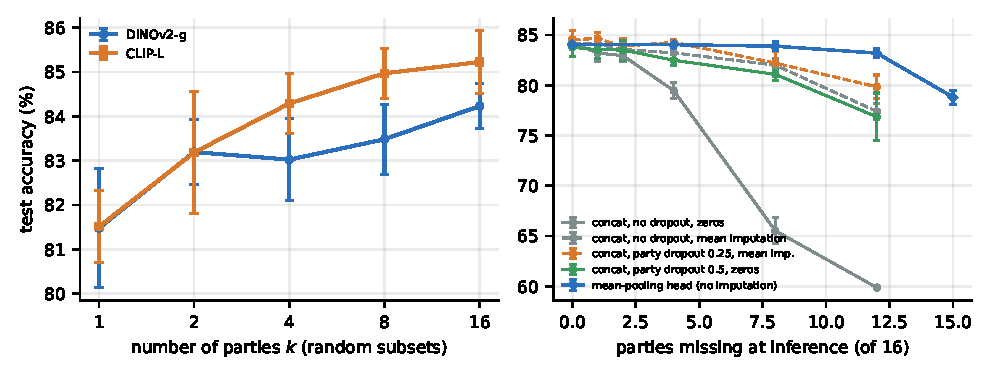
\includegraphics[width=\linewidth]{gen/fig_parties.pdf}
\caption{VertiBench, DINOv2-g. Left: accuracy with $k$ randomly chosen parties (3 subsets $\times$ 5 seeds). Right: parties missing at inference for a concatenation head (missing uploads replaced by zeros or by the party's training mean, with and without party dropout during training) and for a head that averages per-party embeddings.}\label{fig:parties}
\end{figure}

\FloatBarrier

\section{Compression grid}\label{app:pca}

This appendix supports contribution C1: it gives the full grid of local PCA and quantisation from which the main text takes the knee of the frontier, and the limits of compressing without coordination.

\paragraph{Protocol.}
Because the encoder is frozen, each party can fit a PCA on its own training features (keeping $d'\le d$ components; the basis stays with the party) and quantise every coordinate uniformly to $b$ bits between its 1st and 99th training percentiles. The label owner trains the head on the de-quantised values. No labels, shared basis or coordination are needed, but the samples must still be aligned across parties; the few hundred bytes of quantiser bounds that each party sends once are not counted.

\paragraph{Selection under a byte budget.}
On frozen DINOv2-g features we run the grid of Table~\ref{tab:pareto} (16 to 512 components or no PCA, 1 to 16 bits) and select, under each budget, the configuration with the best \emph{validation} accuracy (Fig.~\ref{fig:pareto}). For the 16 parties together, 256\,B per sample (\selTwoCfg) give \selTwoAcc\,\%, 512\,B (\selFiveCfg) \selFiveAcc\,\%, 2\,KiB (\selTwokCfg) \selTwokAcc\,\%, and the full budget selects \selFullCfg{} (\selFullBytes) at \selFullAcc\,\%, against \fullAcc\,\% for the uncompressed 48\,KiB. Moderate compression therefore costs nothing on this benchmark; with 4 bits or more, the PCA-256 and PCA-512 rows are even slightly above the uncompressed features, which we attribute, without having tested it, to a regularising effect on the small labelled set. Even one bit per feature keeps \cmpOneBit\,\%.

\paragraph{Other benchmarks.}
Compression is not free everywhere. On MILK10k a per-party PCA-256 slightly lowers the macro F1 of the concatenation head (\mrGPca, \mrCPca{} and \mrMPca\,\% against \mrGCat, \mrCCat{} and \mrMCat\,\% with DINOv2-g, CLIP-L and MONET; Table~\ref{tab:milkreg}). On WorldStrat, PCA-256 per party changes IPCC and LCCS F1 by \wpIpccPca{} and \wpLccsPca{} points relative to concatenation of the same inputs (Table~\ref{tab:wsfusion}).

\paragraph{Missing parties.}
A concatenation head breaks when parties are missing at inference and their uploads are replaced by zeros (\missZeroEightZ\,\% with 8 of 16 missing, \missZeroTwelveZ\,\% with 12); imputing the party's training mean (\missZeroTwelveM\,\% with 12 missing) or training with party dropout 0.5 (\missHTwelveZ\,\%) repairs most of it (Fig.~\ref{fig:parties}, right). A pooling head (App.~\ref{app:repro}) needs neither: it reaches \poolGMean\,\% with all parties, \poolMissTwelve\,\% with 12 missing and still \poolMissFifteen\,\% with a single party left. It requires a shared feature space, however, and uncoordinated compression removes it: after per-party PCA-64, whose bases differ between parties, the pooling head drops to \poolGPcaMean\,\%, while concatenation of the same uploads keeps \poolGPcaConcat\,\%. Nor does it apply to parties with different modalities or encoders. Local compression and robustness to missing parties must thus be traded off, unless the parties agree on a common basis (e.g.\ one fitted on public images; not tested).

\begin{figure}[tbp]
\centering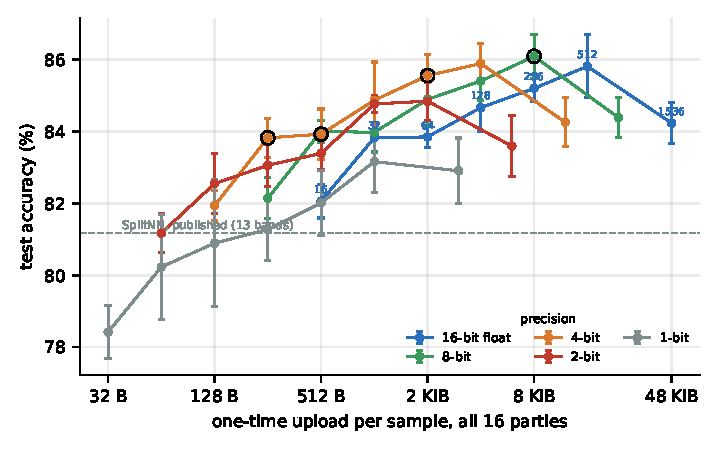
\includegraphics[width=0.78\linewidth]{gen/fig_pareto.pdf}
\caption{VertiBench: accuracy versus one-time upload (bytes per sample, 16 parties) for per-party PCA (number of components annotated on the 16-bit curve) and uniform scalar quantisation of frozen DINOv2-g features, MLP head, 5 seeds. Circles: configuration with the best \emph{validation} accuracy under a budget of 256\,B, 512\,B, 2\,KiB and 48\,KiB.}\label{fig:pareto}
\end{figure}

\begin{table}[tbp]
\caption{The compression grid of Fig.~\ref{fig:pareto} (VertiBench, DINOv2-g, MLP head, 5 seeds). $d'$: PCA components per party (1536: no PCA); $b$: bits per coordinate; upload: one-time payload per sample over the 16 parties. Validation accuracy (seed mean) is the selection criterion; test accuracy and AUC are mean\,$\pm$\,std.}\label{tab:pareto}
\centering\scriptsize
\setlength{\tabcolsep}{4pt}
\begin{tabular}{@{}rrrccc@{}}
\toprule
$d'$ & $b$ & Upload & Val.\ acc.\ (\%) & Test acc.\ (\%) & AUC (\%)\\
\midrule
\inputtab{gen/tab_pareto.tex}
\bottomrule
\end{tabular}
\end{table}

\FloatBarrier

\section{VertiBench audit}\label{app:audit}

This appendix supports contribution C2: it details the audit of the official VertiBench Satellite split and the paired tests behind the comparisons with SplitNN in the main text.

\paragraph{Mapping to source areas.}
Image fingerprints match \auMapTrain{} training and \auMapTest{} test samples to distinct WorldStrat areas (5th-percentile correlation \auScore); \auMapOverlap{} areas appear in both splits.

\paragraph{Siblings, confounded with class.}
The split is not grouped by site, however: \auSibN{} test samples (\auSibShare\,\%) have a training tile from the same site, all from the two sources whose sites are cut into $3\times3$ tiles. They account for \auSibN{} of the 113 test samples in classes 0 and 1, so the \auNoSibN{} test samples without a known sibling are almost all of classes 2 and 3, and class and sibling effects cannot be separated. Table~\ref{tab:audit} gives each head's accuracy on the two subsets. SplitNN is markedly more accurate with siblings (\auSnSib{} vs.\ \auSnNoSib\,\%); the one-shot heads are similarly accurate on both (CLIP-L: \auClipSib{} vs.\ \auClipNoSib\,\%), and the four-logit CLIP heads and frozen split learning are \emph{less} accurate with siblings. The margins over SplitNN are therefore larger on the subset without siblings.

\paragraph{Paired tests.}
The three-seed SplitNN re-run that retains test probabilities averages \auSnAll\,\% accuracy, versus \reproAcc\,\% over five seeds in Table~\ref{tab:main}. We pair test predictions after averaging probabilities over the same three seeds per method (exact McNemar test and 95\,\% paired bootstrap interval, 10{,}000 resamples). On the whole test set, the two CLIP one-shot MLPs, the three four-logit heads and CLIP-B split learning with LoRA beat SplitNN at the 5\,\% level; DINOv2-g's one-shot MLP ($+\pairSnGDiff$ points, $p\pairSnGP$) and frozen CLIP-B split learning do not (Table~\ref{tab:audit}). In detail, the CLIP-L, CLIP-B and DINOv2-g one-shot heads gain $\pairSnClipDiff$ ($p\pairSnClipP$), $\pairSnClipBDiff$ ($p\pairSnClipBP$) and $\pairSnGDiff$ points ($p\pairSnGP$); the CLIP-L, DINOv2-g and CLIP-B four-logit heads give $p\pairSnLgClipP$, $p\pairSnLgGP$ and $p\pairSnLgClipBP$, LoRA split learning $p\pairSnLoraP$ and frozen split learning $p\pairSnSplitFrozenP$. Without known siblings every margin grows and all are significant (CLIP-L: $\pairSnClipNoSibDiff$ points, $p\pairSnClipNoSibP$). These $p$-values are uncorrected: after a Holm correction over the \holmN{} comparisons, \holmSurvive{} remain below 0.05, LoRA split learning and the CLIP-B four-logit head. LoRA itself is unstable across seeds (\seedLoraMin{} to \seedLoraMax\,\%); paired with the ensemble of the one-shot CLIP-B head on the same seeds, its lead is $\pairLoraHeadDiff$ points ($[\pairLoraHeadLo,\pairLoraHeadHi]$, $p\pairLoraHeadP$).

\paragraph{Nearest public image.}
The retrieval attacker of App.~\ref{app:privacy} does not owe its success to siblings: across test uploads, the label of the nearest public training image in CLIP-L space matches in \nnPubAll\,\% of the cases (\nnPubSib\,\% with known siblings, \nnPubNoSib\,\% without), and the neighbour is itself a sibling in just \nnPubIsSib\,\% of the sibling cases, about 5\,\% overall.

\begin{table}[tbp]
\caption{VertiBench audit. Test accuracy (\%) on all 785 test samples, on the \auSibN{} with a training tile from the same site and on the \auNoSibN{} without; paired gain over SplitNN in points with 95\,\% paired bootstrap interval and exact McNemar test, on all samples and without siblings. Probabilities averaged over 3 seeds per method.}\label{tab:audit}
\centering\scriptsize
\setlength{\tabcolsep}{3pt}
\begin{adjustbox}{max width=\linewidth}
\begin{tabular}{@{}lccccccc@{}}
\toprule
& \multicolumn{3}{c}{Accuracy (\%)} & \multicolumn{2}{c}{Gain over SplitNN, all} & \multicolumn{2}{c@{}}{Gain, no sibling}\\
\cmidrule(lr){2-4}\cmidrule(lr){5-6}\cmidrule(l){7-8}
Head & all & sibling & no sibling & points [95\,\% CI] & McNemar & points [95\,\% CI] & McNemar\\
\midrule
SplitNN, VertiBench recipe & \auSnAll & \auSnSib & \auSnNoSib & -- & -- & -- & --\\
\midrule
One-shot MLP, CLIP-L & \auClipAll & \auClipSib & \auClipNoSib & $\pairSnClipDiff$ $[\pairSnClipLo,\pairSnClipHi]$ & $p\pairSnClipP$ & $\pairSnClipNoSibDiff$ $[\pairSnClipNoSibLo,\pairSnClipNoSibHi]$ & $p\pairSnClipNoSibP$\\
One-shot MLP, CLIP-B & \auClipBAll & \auClipBSib & \auClipBNoSib & $\pairSnClipBDiff$ $[\pairSnClipBLo,\pairSnClipBHi]$ & $p\pairSnClipBP$ & $\pairSnClipBNoSibDiff$ $[\pairSnClipBNoSibLo,\pairSnClipBNoSibHi]$ & $p\pairSnClipBNoSibP$\\
One-shot MLP, DINOv2-g & \auGAll & \auGSib & \auGNoSib & $\pairSnGDiff$ $[\pairSnGLo,\pairSnGHi]$ & $p\pairSnGP$ & $\pairSnGNoSibDiff$ $[\pairSnGNoSibLo,\pairSnGNoSibHi]$ & $p\pairSnGNoSibP$\\
\midrule
Four-logit head, CLIP-L & \auLgClipAll & \auLgClipSib & \auLgClipNoSib & $\pairSnLgClipDiff$ $[\pairSnLgClipLo,\pairSnLgClipHi]$ & $p\pairSnLgClipP$ & $\pairSnLgClipNoSibDiff$ $[\pairSnLgClipNoSibLo,\pairSnLgClipNoSibHi]$ & $p\pairSnLgClipNoSibP$\\
Four-logit head, CLIP-B & \auLgClipBAll & \auLgClipBSib & \auLgClipBNoSib & $\pairSnLgClipBDiff$ $[\pairSnLgClipBLo,\pairSnLgClipBHi]$ & $p\pairSnLgClipBP$ & $\pairSnLgClipBNoSibDiff$ $[\pairSnLgClipBNoSibLo,\pairSnLgClipBNoSibHi]$ & $p\pairSnLgClipBNoSibP$\\
Four-logit head, DINOv2-g & \auLgGAll & \auLgGSib & \auLgGNoSib & $\pairSnLgGDiff$ $[\pairSnLgGLo,\pairSnLgGHi]$ & $p\pairSnLgGP$ & $\pairSnLgGNoSibDiff$ $[\pairSnLgGNoSibLo,\pairSnLgGNoSibHi]$ & $p\pairSnLgGNoSibP$\\
\midrule
Split learning, CLIP-B frozen & \auSplitFrozenAll & \auSplitFrozenSib & \auSplitFrozenNoSib & $\pairSnSplitFrozenDiff$ $[\pairSnSplitFrozenLo,\pairSnSplitFrozenHi]$ & $p\pairSnSplitFrozenP$ & $\pairSnSplitFrozenNoSibDiff$ $[\pairSnSplitFrozenNoSibLo,\pairSnSplitFrozenNoSibHi]$ & $p\pairSnSplitFrozenNoSibP$\\
Split learning, CLIP-B LoRA & \auLoraAll & \auLoraSib & \auLoraNoSib & $\pairSnLoraDiff$ $[\pairSnLoraLo,\pairSnLoraHi]$ & $p\pairSnLoraP$ & $\pairSnLoraNoSibDiff$ $[\pairSnLoraNoSibLo,\pairSnLoraNoSibHi]$ & $p\pairSnLoraNoSibP$\\
\bottomrule
\end{tabular}
\end{adjustbox}
\end{table}

\FloatBarrier

\section{MILK10k details}\label{app:milk}

This appendix supports contribution C1: it gives the party combinations, fusion heads and regularisation checks behind the frozen MILK10k rows of Table~\ref{tab:freeze}, and the same-recipe comparison of frozen and adapted backbones. Figure~\ref{fig:frontier-axes-milk} places the MILK10k points on the other axes of the cost accounting: one-shot points need \frMilkRoundsMatch{} message against \frMilkRoundsSplitNN{} for ResNet-18 split learning, and \frMilkGflopsMatchName{} exceeds that baseline (\frMilkGflopsMatchAcc{} vs.\ \frMilkBestNonFound\,\%) with \frMilkGflopsRatio{} times less party compute.

\begin{figure}[t]
\centering\IfFileExists{gen/fig_frontier_axes_milk.pdf}{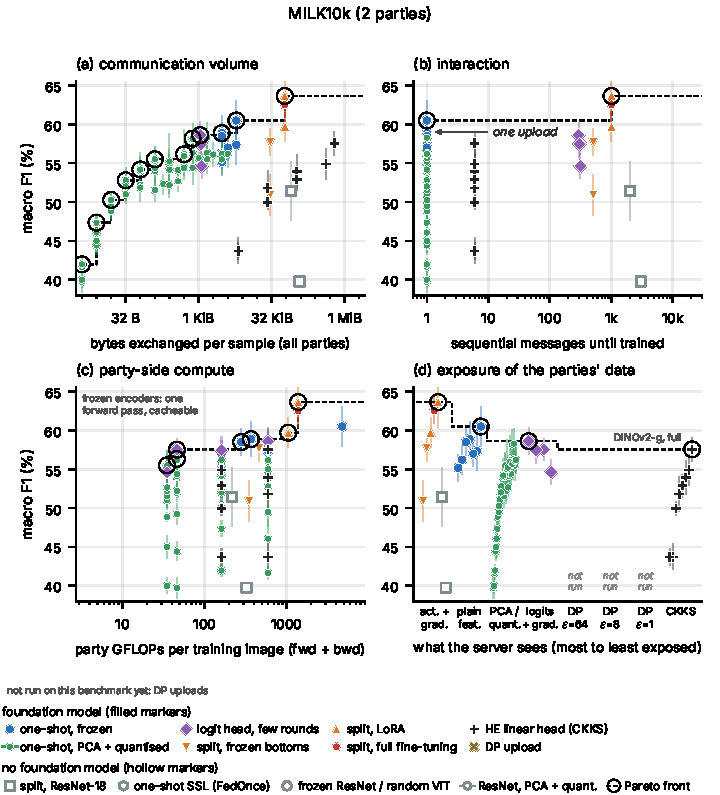
\includegraphics[width=\linewidth]{gen/fig_frontier_axes_milk.pdf}}{\fbox{\parbox{0.9\linewidth}{\centering fig\_frontier\_axes\_milk pending}}}
\caption{MILK10k along the axes of Fig.~\ref{fig:frontier-axes}: (a)~bytes per training sample, (b)~sequential messages until trained, (c)~party GFLOPs per training image (forward and backward), (d)~exposure ladder. Only DP is marked as not run. Circled: Pareto-optimal points.}\label{fig:frontier-axes-milk}
\end{figure}

\begin{table}[tbp]
\caption{MILK10k, all methods (2 parties, 5 folds, class-balanced loss). Split learning trains the bottoms with the server's gradients; one-shot rows use frozen features and an MLP head (concatenation, or late fusion on features averaged over 8 rotations and flips). Upload per training sample: over all training epochs for split learning (30 for ResNet-18 from scratch, 20 from ImageNet, 10 for ViTs), once for one-shot. Time: minutes per fold (one-shot: encoding, estimated).}\label{tab:freeze}
\centering\scriptsize
\setlength{\tabcolsep}{3pt}
\begin{adjustbox}{max width=\linewidth}
\begin{tabular}{@{}llrrrccc@{}}
\toprule
Party models & Training & Trainable & Upload & Time & F1 (\%) & Bal.\ acc.\ (\%) & Acc.\ (\%)\\
\midrule
\inputtab{gen/tab_freeze.tex}
\bottomrule
\end{tabular}
\end{adjustbox}
\end{table}

\paragraph{Real modalities complement each other little.}
The dermoscopic image alone gives \milkGDerm\,\% macro F1 with DINOv2-g, the clinical photograph \milkGClin\,\%, the metadata \milkMeta\,\% (Table~\ref{tab:milk}). Concatenating the two images adds less than one point over the dermoscopy (\milkGBoth\,\%), three points with CLIP-L (\milkCDerm{} $\to$ \milkCBoth\,\%); the metadata add at most one point on top. The general-purpose encoders match or beat the medical ones (BiomedCLIP, MONET). Splitting the dermoscopy into two halves, as split benchmarks do, \emph{loses} information instead: \milkGHalves\,\% against \milkGDerm\,\% for the whole image, because each party's encoder sees half a lesion. Two caveats apply to all MILK10k numbers: folds are drawn over lesions, as the release has no patient identifiers, and each test fold holds only 40 to 61 lesions of the two rarest classes.

\paragraph{How the parties are combined matters as much as the encoder.}
A concatenation MLP under-uses the weaker party. Training one head per party and averaging their log-probabilities (late fusion) is better for every encoder (Table~\ref{tab:milkfusion}): \mfGLate\,\% instead of \mfGCat\,\% with DINOv2-g, \mfCLate\,\% instead of \mfCCat\,\% with CLIP-L, \mfGMLate\,\% when each party uploads DINOv2-g and MONET features; with DINOv2-g, the two parties together then reach \mfGLate\,\%, about three points more than the dermoscopic party alone (\milkGDerm\,\%). Late fusion also suits VFL: each party's head can be trained, audited and dropped independently. The gain is bounded by the data: \mfGBoth\,\% of the lesions are misclassified by both single-party heads, against \mfGIndep\,\% if their errors were independent---the two modalities fail on the same, intrinsically hard lesions.

\paragraph{Over-fitting or modality competition?}
With 3{,}100 training lesions and 2--3k input dimensions, the concatenation head could simply over-fit. Three observations speak against this being the main cause (Table~\ref{tab:milkreg}). First, regularising it---input dropout, Gaussian feature noise, feature mixup, a per-party PCA---gains at most one point and never reaches late fusion. Second, late fusion does not need its tuned weight: a fixed weight of 0.5 does as well (\mrGLateHalf\,\% with DINOv2-g); paired by fold, it beats concatenation by \mrGPairD\,$\pm$\,\mrGPairS{} points with DINOv2-g (\mrGPairW{} folds out of 5), \mrCPairD\,$\pm$\,\mrCPairS{} with CLIP-L (\mrCPairW/5) and \mrMPairD\,$\pm$\,\mrMPairS{} with MONET (\mrMPairW/5). Third, its advantage does not shrink with more data, as over-fitting would predict: it grows from 25\,\% to 100\,\% of the training folds for CLIP-L and MONET. Nor is it an artefact of our early-stopping rule on the unweighted validation loss: when both heads stop on the class-weighted validation loss or on the validation macro F1, late fusion still wins by \mrStopMin{} to \mrStopMax{} points over \mrStopN{} comparisons (DINOv2-g, CLIP-L, DINOv2-B, CLIP-B; stopping on the weighted loss lowers every head by up to \mrWlossDropMax{} points), and weight decay on the concatenation head leaves a gap of \mrWdMin{} to \mrWdMax{} points. The pattern rather matches the \emph{modality competition} documented for jointly trained multimodal networks~\cite{wang2020makes,huang2022modality,peng2022balanced}: a joint head learns the dominant dermoscopy first and stops before exploiting the clinical photograph, whereas separate heads must each use their own modality fully; the validation-tuned late fusion gives the weaker clinical party a weight of 0.3 to 0.5. Augmentation helps in image space, not in feature space: the parties can encode the 8 rotations and flips of each photograph once (8 times the encoding cost) and upload the mean, which raises late fusion to \mrGLateViews\,\% (DINOv2-g), \mrMLateViews\,\% (MONET), \fzViewsB\,\% (DINOv2-B) and \fzViewsCb\,\% (CLIP-B) at no extra communication. With CLIP-L it helps late fusion little (\mrCLateViews\,\%); there the best head is the concatenation trained on one of the 8 uploaded views per epoch (\mrCCatSampled\,\%, at 8 times the upload).

\paragraph{Frozen versus adapted under the same recipe.}
The frozen and adapted rows of Table~\ref{tab:freeze} differ in more than freezing (augmentation, head, standardisation, optimiser and schedule). In a paired re-run we therefore use the same split-learning recipe with frozen and LoRA bottoms. For DINOv2-B this gives \srFrozenB\,\% macro F1 frozen versus \srLoraB\,\% with LoRA (paired gain $\srGapB\pm\srGapSdB$ points, \srWinsB/5 folds); for CLIP-B, \srFrozenCb\,\% versus \srLoraCb\,\% ($\srGapCb\pm\srGapSdCb$ points, \srWinsCb/5 folds). Relative to the one-shot MLPs, freezing under the split recipe shifts F1 by $\srVsHeadB$ and $\srVsHeadCb$ points, respectively, so the larger same-recipe LoRA gain for CLIP-B partly reflects its weaker frozen baseline under that recipe. Adaptation wins on MILK10k under both recipes.

\begin{table}[tbp]
\caption{MILK10k: macro F1 (\%) of one-shot heads on frozen features for every combination of parties (5 folds, class-balanced MLP head). Bottom: the usual practice of splitting one image into a left and a right party.}\label{tab:milk}
\centering\scriptsize
\setlength{\tabcolsep}{3.5pt}
\begin{adjustbox}{max width=\linewidth}
\begin{tabular}{@{}lcccc@{}}
\toprule
Parties & \inputtab{gen/tab_milk_head.tex}\\
\midrule
\inputtab{gen/tab_milk.tex}
\bottomrule
\end{tabular}
\end{adjustbox}
\end{table}

\begin{table}[tbp]
\caption{MILK10k: how the label owner combines the clinical (A) and dermoscopic (B) uploads (macro F1, \%, 5 folds). Late fusion: one head per party, log-probabilities averaged with a weight chosen on the validation fold. Branches: per-party projection, auxiliary per-party losses and modality dropout (0.3). Last column: share of test lesions misclassified by both single-party heads, and (in brackets) what it would be if their errors were independent.}\label{tab:milkfusion}
\centering\scriptsize
\setlength{\tabcolsep}{3pt}
\begin{adjustbox}{max width=\linewidth}
\begin{tabular}{@{}lcccccc@{}}
\toprule
Encoder & B alone & A+B concat & A+B late fusion & A+B branches & A+B+C branches & Both wrong (\%)\\
\midrule
\inputtab{gen/tab_milkfusion.tex}
\bottomrule
\end{tabular}
\end{adjustbox}
\end{table}

\begin{table}[tbp]
\caption{MILK10k, clinical + dermoscopic parties: is the concatenation head over-fitting? Macro F1 (\%, 5 folds). Top: regularising the concatenation head versus late fusion. Middle: augmentation precomputed once by the parties (8 rotations and flips of each photograph). Bottom: gap between late fusion (fixed weight) and concatenation when the training folds are subsampled, and under other early-stopping rules than the unweighted validation loss.}\label{tab:milkreg}
\centering\scriptsize
\setlength{\tabcolsep}{3.5pt}
\begin{adjustbox}{max width=\linewidth}
\begin{tabular}{@{}lccc@{}}
\toprule
Head & DINOv2-g & CLIP-L & MONET\\
\midrule
\inputtab{gen/tab_milkreg.tex}
\bottomrule
\end{tabular}
\end{adjustbox}
\end{table}

\FloatBarrier

\section{WorldStrat: two sensors}\label{app:ws}

This appendix supports contribution C2: it reports a third natural partition, with genuinely different sensors, on which the two parties complement each other little once the folds are grouped by site.

\paragraph{Task.}
From the WorldStrat release~\cite{cornebise2022worldstrat} we build a two-party task on its \wsIpccN{} usable areas of $1.58\times1.58$\,km: party A holds the SPOT 6/7 pan-sharpened image (RGB, 1.5\,m, $1050\times1050$ pixels), party B the 16 Sentinel-2 L1C revisits (13 bands, 10\,m). The label owner holds one of three labels of the release metadata, all read at the centre of the area: the LCCS land-cover class of the 300\,m pixel of a global land-cover map~\cite{esa2017cci} (the 18 classes with at least 40 areas), its coarser IPCC category (7 classes), and the degree of urbanisation of the 1\,km SMOD cell (8 classes, from rural very-low-density to urban centre~\cite{pesaresi2019ghsl}). A label therefore describes only the centre of the image (4\,\% of its area for LCCS and IPCC); the parties also encode centre crops of 336\,m and 1\,km. To vary the information held by A, its image is degraded to 3, 6 and 10\,m before encoding, or cut into 16 full-resolution tiles of 262\,px whose features are averaged. Party B encodes every revisit as three composites (RGB, near- and short-wave infrared) and uploads, per composite, the mean over the 16 revisits or over the 8 least cloudy ones (ranked by a locally computed cloud score), possibly with the temporal standard deviation; for a set head it uploads all 16 vectors. The loss is class-balanced and macro F1 is the metric.

\paragraph{Grouped cross-validation.}
The five folds are stratified and grouped by site: all nine tiles of a site stay in the same fold. Stratification alone split sibling tiles across training and test and gave macro F1 about 6 to 9 points higher on the two land-cover tasks---the same leakage as in the official VertiBench split, which is built from the same areas (App.~\ref{app:audit}). All results below are site-grouped and paired by fold.

\paragraph{The second sensor adds little.}
Alone, the 1.5\,m SPOT image scores \wsIpccSpot{} against \wsIpccSms\,\% macro F1 for the Sentinel-2 revisits (RGB, NIR, SWIR) on IPCC, \wsLccsSpot{} against \wsLccsSms\,\% on LCCS and \wsSmodSpot{} against \wsSmodSms\,\% on SMOD (Table~\ref{tab:ws}). Their concatenation reaches \wsIpccFus, \wsLccsFus{} and \wsSmodFus\,\%: relative to SPOT, F1 changes by \wgIpccA{} points on IPCC (\wgIpccAW{} folds improve), \wgLccsA{} on LCCS (\wgLccsAW) and \wgSmodA{} on SMOD (\wgSmodAW). With DINOv2-g, the pair is thus at most a couple of points above the better single sensor on land cover, and below SPOT alone on urbanisation. The second sensor matters more when the first is weakened (Fig.~\ref{fig:ws}): at 3\,m, fusion adds \wgIpccThree{} points on IPCC (\wgIpccThreeW) and \wgLccsThree{} on LCCS (\wgLccsThreeW); at 10\,m, \wgIpccTen{} (\wgIpccTenW) and \wgLccsTen{} (\wgLccsTenW), whereas SMOD never gains (\wgSmodTen{} at 10\,m, \wgSmodTenW). For land cover, SPOT improves alone at 3\,m (\wsIpccSpotThree{} and \wsLccsSpotThree\,\%) or by averaging the features of 16 full-resolution tiles (\wfIpccSpotTiles{} and \wfLccsSpotTiles\,\%), rather than feeding DINOv2 the whole 1{,}050\,px image; adding the clearest revisits to the tiles yields \wpIpccTilesFus{} and \wpLccsTilesFus{} points (\wpIpccTilesFusW{} and \wpLccsTilesFusW). Adding infrared to RGB helps LCCS at native resolution and both land-cover labels at 10\,m. With a multispectral encoder (SSL4EO-S12 on the 13 bands) for party B, or CLIP-L for both parties, fused IPCC scores and their gain over the single sensors are larger (Table~\ref{tab:ws}), while SMOD barely changes; we did not test these rows in pairs. For native-resolution fusion, pooled out-of-fold per-class F1 gains over SPOT are largest for \wcIpccTop{} on IPCC and \wcLccsTop{} on LCCS (points and number of areas); F1 falls in \wcIpccNeg{} IPCC and \wcLccsNeg{} LCCS classes.

\paragraph{Why a second sensor adds little.}
The parties fail on the same areas: on IPCC both are wrong on \wfIpccBoth\,\% of them, nearly three times the \wfIpccIndep\,\% expected from independent errors, although an oracle choosing the right party would reach \wfIpccOracle\,\% accuracy. Context matters more than a second view of the labelled pixel: although labels are read at the centre of the area, the whole 1.58\,km SPOT image beats a 336\,m centre crop by \wpIpccCentre, \wpLccsCentre{} and \wpSmodCentre{} points (\wpIpccCentreW, \wpLccsCentreW{} and \wpSmodCentreW{} folds); with a 1\,km crop, land-cover scores are roughly unchanged and only SMOD still loses ground (\wfSmodSpotCk{} vs.\ \wfSmodSpot\,\%).

\paragraph{Fusion heads do not change the picture.}
No fusion variant of Table~\ref{tab:wsfusion} improves on plain-mean concatenation across all three labels. The set head over the 16 revisits changes F1 by \wpLccsSetCat{} to \wpIpccSetCat{} points while multiplying the Sentinel-2 payload by 16. Late fusion changes IPCC, LCCS and SMOD F1 by \wpIpccLateMean, \wpLccsLateMean{} and \wpSmodLateMean{} points with the plain mean (SMOD improves in \wpSmodLateMeanW{} folds), and by \wpIpccLateCat, \wpLccsLateCat{} and \wpSmodLateCat{} with the clearest-revisit summary, where the branch head trails concatenation by \wpIpccBranch, \wpLccsBranch{} and \wpSmodBranch{} points. Adding temporal standard deviations shifts the IPCC F1 of Sentinel-2 alone by \wpIpccStdSolo{} points (\wpIpccStdSoloW{} folds improve), and adding a centre crop to SPOT alone changes IPCC and LCCS by \wpIpccFC{} and \wpLccsFC{} points.

\begin{table}[tbp]
\caption{WorldStrat, 5 site-grouped folds: macro F1 (\%, mean\,$\pm$\,std) of each sensor alone and of their concatenation (MLP head; DINOv2-g unless noted). A: SPOT image; B: mean of the 16 Sentinel-2 revisits, encoded as RGB, as three composites (RGB, NIR, SWIR) or on all 13 bands by SSL4EO-S12. Note the column order.}\label{tab:ws}
\centering\scriptsize
\setlength{\tabcolsep}{4pt}
\begin{tabular}{@{}lccc@{}}
\toprule
Parties & IPCC & SMOD & LCCS\\
\midrule
\inputtab{gen/tab_ws.tex}
\bottomrule
\end{tabular}
\end{table}

\begin{figure}[tbp]
\centering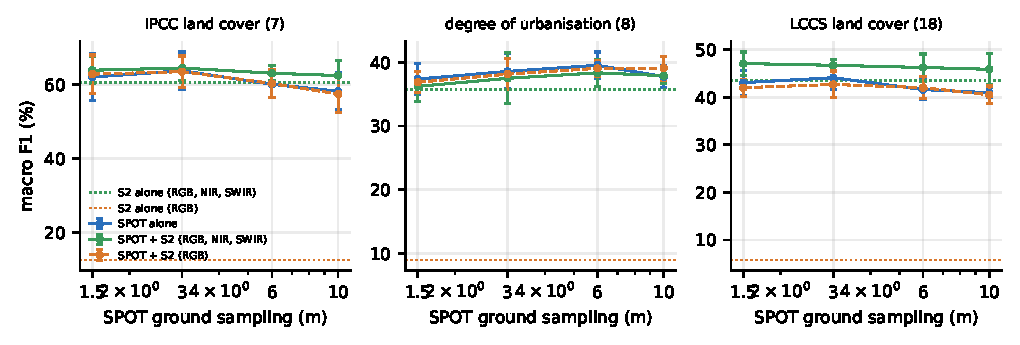
\includegraphics[width=\linewidth]{gen/fig_ws.pdf}
\caption{WorldStrat: macro F1 (mean over 5 site-grouped folds, DINOv2-g, MLP head) of the SPOT party alone and with the Sentinel-2 party, as the SPOT image is degraded from 1.5 to 10\,m. Dotted: Sentinel-2 alone. Fold standard deviations are about 1 to 6 points; paired differences are given in the text.}\label{fig:ws}
\end{figure}

\begin{table}[tbp]
\caption{WorldStrat: single parties and fusion heads (macro F1, \%, mean\,$\pm$\,std over 5 site-grouped folds, DINOv2-g). S2 vectors: number of 4{,}608-d vectors (RGB, NIR and SWIR composites) the Sentinel-2 party uploads per area; the SPOT party uploads one 1{,}536-d vector (two with the centre crop, three with three scales). C: whole SPOT image and mean of the 8 least cloudy revisits. All variants remain one-shot.}\label{tab:wsfusion}
\centering\scriptsize
\setlength{\tabcolsep}{3pt}
\begin{adjustbox}{max width=\linewidth}
\begin{tabular}{@{}lcccc@{}}
\toprule
Configuration & S2 vectors & IPCC & LCCS & SMOD\\
\midrule
\inputtab{gen/tab_wsfusion.tex}
\bottomrule
\end{tabular}
\end{adjustbox}
\end{table}

\FloatBarrier

\section{Classic split benchmarks}\label{app:classic}

This appendix supports contribution C2 by showing why natural benchmarks are needed: on the classic CIFAR and ModelNet40 splits, the gains of a single upload of frozen features mostly measure pre-training.

\paragraph{Splits.}
CIFAR-10/100~\cite{krizhevsky2009cifar} are split as in the papers we compare with: top/bottom halves ($K=2$) and $16\times16$ quadrants ($K=4$) as in VFLAIR~\cite{zou2024vflair} and FedOnce~\cite{wu2022fedonce}, and left/right halves with only $N_o\in\{256,\dots,2048\}$ aligned labelled samples as in Sun et al.~\cite{sun2023oneshotvfl}. Halves are upsampled by 7 ($16\times32\to112\times224$) and quadrants by 14 ($16\times16\to224\times224$), so four quadrants are encoded with four times as many tokens as two halves ($4\times256$ against $2\times128$). ModelNet40~\cite{wu2015modelnet} uses 12 rendered views per object~\cite{su2015mvcnn} (9{,}843 training and 2{,}468 test objects), one view per party ($K=12$) or three per party ($K=4$). We quote the published numbers of the original papers, including VIMADMM~\cite{xie2024vimadmm}.

\paragraph{Large gains that mostly measure pre-training.}
Frozen DINOv2-g features beat every published number by a wide margin (Table~\ref{tab:classic}): \cTenGTwo\,\% on CIFAR-10 cut into top and bottom halves (VFLAIR's split learning: 79.8\,\%), \cTenGFour\,\% with four quadrants (VFLAIR: 76.2\,\%, FedOnce: 58.7\,\%), and \sunA\,\% with only 256 aligned labelled samples, where the semi-supervised three-message protocol of Sun et al.\ reaches 78--80\,\%. On CIFAR-100 the margin is wider still (\cHunGTwo\,\% and \cHunGFour\,\% against 42.3 and 38.2\,\% for VFLAIR), and on ModelNet40 with three views per party DINOv2-g reaches \mnGFour\,\% against 91.3\,\% for VIMADMM and 90.0\,\% for split learning with trained ResNet-18 bottoms. For DINOv2-g, four parties do better than two on CIFAR-100, possibly because the four uploads describe the image with four times as many tokens; we did not test this at an equal token budget, and CLIP-L goes the other way (\cHunCTwo{} to \cHunCFour\,\%). CLIP-L is less robust to small upsampled pieces (\cHunCFour\,\% on CIFAR-100 quadrants against \cHunCCent\,\% on full images), DINOv2-g much more (\cHunGFour{} against \cHunGCent\,\%). These gains should not be over-interpreted: the published baselines train small encoders from scratch, and CIFAR's classes are central to web-scale pre-training data, so a split CIFAR benchmark mostly measures the encoder's pre-training. The splits also create complementarity by construction: one CIFAR-10 quadrant alone gives \cTenGSoloQ\,\%, the four together \cTenGFour\,\%, whereas real parties often see the same object almost completely (App.~\ref{app:milk}). Hence the main text uses naturally partitioned data.

\begin{table}[tbp]
\caption{Classic split benchmarks: one upload of frozen features (224\,px, MLP head, 3 seeds; 5 seeds for the protocol of Sun et al.) against the published numbers of methods that train the party models, under the same splits. CIFAR halves are upsampled to $112\times224$, quadrants to $224\times224$; ModelNet40 uses 12 rendered views. Bottom: left/right CIFAR-10 halves with $N_o$ aligned labelled samples.}\label{tab:classic}
\centering\scriptsize
\setlength{\tabcolsep}{3pt}
\begin{adjustbox}{max width=\linewidth}
\begin{tabular}{@{}llp{4.3cm}cc@{}}
\toprule
Data & Split & Published (acc.\,\%) & DINOv2-g & CLIP-L\\
\midrule
\inputtab{gen/tab_classic.tex}
\bottomrule
\end{tabular}
\end{adjustbox}

\vspace{4pt}
\begin{adjustbox}{max width=\linewidth}
\begin{tabular}{@{}rcccc@{}}
\toprule
Aligned samples $N_o$ & Sun et al.\ one-shot & Sun et al.\ few-shot & DINOv2-g & CLIP-L\\
\midrule
\inputtab{gen/tab_sun.tex}
\bottomrule
\end{tabular}
\end{adjustbox}
\end{table}

\FloatBarrier

\section{Privacy details}\label{app:privacy}

This appendix supports contribution C1: it details the attacks on plaintext uploads, the party-side transforms, the differential-privacy mechanism and the parameters and cost of encrypted training that place the regimes on the exposure axis.

\subsection{Attacks on plaintext uploads}

\paragraph{Linkage.}
An attacker holding public copies of the candidate images needs no decoder: encoding them with the public encoder and matching the uploads links each upload to its image. Exact re-encoding links \giLink\,\% of the uploads within one party. Across the full gallery of the \lkN{} test images of the 16 parties, top-1 linkage rounds to \lkSame\,\% with identical preprocessing (\lkDup{} uploads have duplicates), versus \lkBicubic\,\% after bicubic resizing, \lkEightbit\,\% after 8-bit quantisation of the resized image and \lkClip\,\% with CLIP's standard preprocessing of the same encoder; within a single party, even the worst party still links \lkClipParty\,\% under that last mismatch.

\paragraph{Generic decoder.}
The encoders are public, so the attacker does not need in-domain pairs either: for OpenAI CLIP ViT-L/14, Stable unCLIP~2.1 (``small'')~\cite{ramesh2022unclip,rombach2022ldm} generates an image from the CLIP image embedding, which is the pooled output a party uploads times the public projection matrix of the encoder. We decode, without any adaptation, the CLIP-L uploads of \giVbN{} VertiBench test images of one party and of \giMilkN{} MILK10k test lesions per modality (25 denoising steps, guidance scale~10, empty text prompt). Pixel metrics say little about a generator that does not reproduce brightness or exact layout, so we measure what the attacker learns with an independent encoder, DINOv2 ViT-B/14: re-identification of the source among all candidates (the \giVbNTest{} test images of the party, all \giMilkNGal{} MILK10k lesions) by the cosine of DINOv2-B features (VertiBench images contrast-stretched per channel), and the label predicted from the reconstruction by a logistic regression trained on the DINOv2-B features of real training images. On VertiBench (Fig.~\ref{fig:generic}) the pixels are lost (PSNR \giVbPsnr\,dB; a reconstruction is closer to its source than to any other test image in \giVbPixReid\,\% of the cases), yet the independent encoder picks the source in \giVbReid\,\% of the cases (top-10: \giVbReidTen\,\%; chance: \giVbChance{} and \giVbChanceTen\,\%), and the label of the reconstruction is predicted with \giVbLabFone\,\% macro F1, against \giVbRealFone\,\% from the image itself and \giVbChanceFone\,\% from the class frequencies. A party that encodes its images with CLIP's own preprocessing rather than ours leaks as much (\giVbClipReid\,\% and \giVbClipLabFone\,\%). On MILK10k the decoder draws skin with a lesion-like spot, but recovers neither the lesion (top-10 re-identification: \giMilkClinReidTen\,\% clinical, \giMilkDermReidTen\,\% dermoscopic) nor its diagnosis (\giMilkClinLabFone{} and \giMilkDermLabFone\,\% macro F1; chance \giMilkChanceFone, real images \giMilkClinRealFone{} and \giMilkDermRealFone\,\%): what a generic decoder recovers depends on how well its training images cover the domain. For the pooled DINOv2 token we found no public decoder---decoders from DINOv2 \emph{patch} tokens~\cite{zheng2026rae} and diffusion-guided attacks on intermediate features~\cite{lei2025drag} exist---so we did not attack DINOv2 uploads this way; it is feasible in principle, by training such a decoder once on public images~\cite{bordes2022rcdm} or by mapping DINOv2 to CLIP embeddings with public images.

\paragraph{Fine-tuned decoder and retrieval.}
On VertiBench we also give the decoder the attacker's best chance: we fine-tune all the weights of its denoising network on public in-domain pairs---the RGB composites of the 16 revisits of \giftLocs{} training locations, standing for public Sentinel-2 images (brightened 1.6 times, at $\giftSize\times\giftSize$ pixels), with their CLIP-L embeddings: \giftPairs{} pairs---with its usual v-prediction loss, for \giftMinutes{} minutes on one GPU (\giftSteps{} steps of 32 pairs, learning rate $10^{-5}$, embedding dropped for 10\,\% of the pairs so that classifier-free guidance still works). Its guidance scale (among \giftGuidGrid) is chosen on 200 other training locations by the cosine between the CLIP-L embeddings of the decoded image and of the source, and the attacker keeps the best of \giftNBest{} samples per upload, the one whose embedding is closest to the upload. The fine-tuned decoder draws Sentinel-2-like composites (Fig.~\ref{fig:generic-ft}) whose CLIP embedding is closer to the upload (cosine \giftBestClip, against \giftOffClip{} for the off-the-shelf decoder at the same \giftSize-pixel resolution, where it fails: \giVbOffLabFone\,\% macro F1) and whose pixels are closer to the source (PSNR \giVbBestPsnr\,dB), as it has learnt their brightness and colours; but it re-identifies the source no more often (\giVbBestReid\,\%, top-10 \giVbBestReidTen\,\%) and predicts its label only slightly better (\giVbBestLabFone\,\% macro F1). The same public pairs give a \emph{retrieval} attacker, which returns the public image whose CLIP-L embedding is nearest to the upload: it is matched back to the source in \giVbNnReid\,\% of the cases by the independent encoder (top-10: \giVbNnReidTen\,\%) and predicts the label with \giVbNnLabFone\,\% macro F1, as well as the real image does; App.~\ref{app:audit} shows that this does not rest on siblings.

\paragraph{Decoders trained on in-domain pairs.}
A curious label owner holding auxiliary image--feature pairs from the same distribution (cheap when the imagery and the encoder are public) can also train decoders from one uploaded vector to the $64\times64$ RGB thumbnail of its party: a deconvolutional network with a pixel-wise MSE loss over the 50k training pairs, trained for \invEpochs{} epochs (AdamW, one-cycle schedule) and shared by all parties, or for \invShortEpochs{} epochs (Adam) with a learned per-party affine input map initialised at the identity (the long variant uses such a map only for per-party PCA, whose bases differ); and a closed-form linear (ridge) decoder, fitted per party for PCA uploads. For compressed uploads the attacker knows the party's PCA basis; for randomised uploads it draws fresh noise at every training step. We report PSNR, SSIM~\cite{wang2004ssim} and two re-identification rates on $16\times16$ thumbnails (source image among the test images; source location among the \invNLoc{} test locations, at any date), calibrated by the mean training image, each image's own mean colour and the nearest training image in feature space. From one full upload, the decoder reaches \invFull\,dB PSNR (Table~\ref{tab:privacy}, Fig.~\ref{fig:inversion}): better than the mean training image (\invMean\,dB) or the nearest training image in feature space (\invNN\,dB), but \emph{worse} than painting each image with its own mean colour (\invColour\,dB); the linear decoder reaches \invLinFull\,dB. The decoder is not under-trained: on its training images its error (MSE \invFullTrainMse) is less than a quarter of that of the mean-colour rendering (\invColourTrainMse), but this does not carry over to unseen images, and training it for \invEpochs{} rather than \invShortEpochs{} epochs gains only \invGainLong\,dB. Reconstructions single out their source among the \lkN{} test images in \invFullReid\,\% of the cases and its location in \invFullReidLoc\,\% (top-10: \invFullReidLocTen\,\%; chance: 0.01, \invChanceLoc{} and \invChanceLocTen\,\%), less often than the mean-colour rendering (\invColourReidLoc{} and \invColourReidLocTen\,\%). Compression lowers this leakage at little cost in accuracy: after PCA-16 the best attacker reaches \invBestPCAst\,dB and finds the location in \invBestPCAstReidLoc\,\% of the cases. A pixel-loss decoder is a weak attacker; these numbers bound the leakage from below.

\subsection{Party-side transforms}

A party can transform its features before uploading them, at no communication cost: a secret random rotation; its own PCA-64 basis; the 100-dimensional code of an autoencoder (MLP, MSE loss) or of a noise-as-targets encoder~\cite{bojanowski2017nat} trained on its own features; or, giving up one-shot training, a linear layer to 100 dimensions trained jointly with the head by split learning. The generic decoder needs CLIP embeddings, so the attacker first learns a map back from the transformed upload. Without any image--upload pair of the party, it matches the eigenvectors of the party's uploads with those of public in-domain features (here the CLIP-L features of the other revisits), in order of eigenvalue and with signs set by the skewness of the projections, which undoes any orthogonal transform up to the ambiguity of close eigenvalues. With $k$ leaked pairs it fits a ridge regression from uploads to CLIP embeddings (or an MLP when $k\ge1{,}000$, if better on held-out pairs).

The rotation costs nothing (\gdRotAcc\,\% accuracy against \gdPlainAcc\,\%), the autoencoder code \gdAeDrop{} points, the private PCA-64 \gdPcaDrop{} and the split-learning bottleneck \gdSplitDrop{} (Table~\ref{tab:defences}). Without leaked pairs, our spectral alignment does not undo them: the embeddings it recovers are further from the true ones (cosine \gdRotCosZero) than the mean embedding is (\giCosMean), and link \gdRotLinkZero\,\% of the uploads; unsupervised alignment methods developed for word embeddings~\cite{conneau2018word,grave2019wasserstein} may do better. With 100 leaked pairs (3\,\% of a party's samples), however, a ridge regression maps the rotation, the PCA and the autoencoder code back to CLIP embeddings that link \gdPcaLinkOneZeroZero{} to \gdAeLinkOneZeroZero\,\% of the uploads (split learning: \gdSplitLinkOneZeroZero\,\%), and 1{,}000 pairs bring all four to at least \gdSplitLinkOneZeroZeroZero\,\% (cosine \gdSplitCosOneZeroZeroZero{} to \gdRotCosOneZeroZeroZero). Only noise as targets resists, with \gdNatLinkThreeOneFourTwo\,\% after all 3{,}142 training pairs, because its codes discard much of the information: they cost \gdNatDrop{} points of accuracy. A transform that preserves accuracy preserves what the attacker needs, and keeping image--upload pairs secret is a weak assumption.

\subsection{Differential privacy of the upload}

Party $k$ clips each vector (raw or after PCA) at the median $\ell_2$ norm $c_k$ of its own training vectors and adds noise $\mathcal{N}(0,\sigma_k^2 I)$. For fixed preprocessing and $c_k$, replacing one record changes the clipped vector by at most $2c_k$, so each release is $\mu$-Gaussian-DP with $\mu=2c_k/\sigma_k$~\cite{dong2022gdp}; we set $\sigma_k$ from a target per-upload $(\varepsilon,\delta=10^{-5})$. The 16 uploads of a sample compose to $4\mu$: a per-upload $\varepsilon=8$ gives $\varepsilon\approx50$ for the sample, and $\varepsilon=64$ gives $\varepsilon\approx630$. These budgets do not account for estimating the clipping norms or fitting the PCA on the training data: the guarantee is formal but loose. Because the clipped signal has a fixed norm while the noise norm grows with the square root of the dimension, PCA is what makes DP usable. On VertiBench with DINOv2-g, a per-upload $\varepsilon=8$ drops the full features to \dpFullEight\,\%, below the \majVB\,\% of always predicting the majority class (the inversion PSNR is then that of the mean training image to the reported precision, and re-identification is near chance; Table~\ref{tab:privacy}), whereas after PCA-16 the same budget keeps \dpStEight\,\%, above it. At $\varepsilon=64$, full features give \dpFullSsf\,\%, PCA-64 \dpSfSsf\,\% and PCA-16 \dpStSsf\,\% (PCA-64 at $\varepsilon=8$: \dpSfEight\,\%). PCA followed by DP is thus the privacy end of the frontier: a formal, loose guarantee at an accuracy cost, whereas the reproduced SplitNN, at \reproAcc\,\%, offers no formal guarantee.

\subsection{Encrypted training of a linear head}

\begin{table}[tbp]
\caption{Heads that can be trained on encrypted uploads: accuracy (VertiBench, CIFAR) or macro F1 (MILK10k, WorldStrat), mean\,$\pm$\,std over 5 seeds or folds (CIFAR: 3 seeds). MLP: reference head re-run in the ridge pipeline (hence tenths of a point from Table~\ref{tab:main}). Ridge: closed form on standardised features (class-weighted on MILK10k and WorldStrat), emulated in plaintext, after a per-party PCA to 256, 64 or 16 components; --: too large to emulate.}\label{tab:he}
\centering\scriptsize
\setlength{\tabcolsep}{4pt}
\begin{adjustbox}{max width=\linewidth}
\begin{tabular}{@{}lccccc@{}}
\toprule
& \multicolumn{2}{c}{Full features} & \multicolumn{3}{c}{Ridge after per-party PCA}\\
\cmidrule(lr){2-3}\cmidrule(lr){4-6}
Task & MLP & Ridge & 256 & 64 & 16\\
\midrule
\inputtab{gen/tab_he.tex}
\bottomrule
\end{tabular}
\end{adjustbox}
\end{table}

\paragraph{Protocol.}
After a local PCA to $d'$ components and standardisation, the ridge classifier $W=(X^\top X+\lambda I)^{-1}X^\top Y$ on one-hot targets only needs $X^\top X$ and $X^\top Y$. Every party encrypts its feature columns once with CKKS under a threshold key generated jointly by the parties~\cite{mouchet2021multiparty} (a single key shared by the passive parties would let each of them decrypt the others' uploads); the label owner computes the cross-party blocks $X_k^\top X_l$ and $X_k^\top Y$ homomorphically (multiplicative depth one), masks them with random matrices, has them decrypted and solves the system in the clear: one upload plus one round trip of $\mathcal{O}(D^2)$ aggregates, $D=Kd'$, and no per-sample feature is ever decrypted. With class weights, which depend on the labels, the label owner also sends the encrypted per-sample weights; every party multiplies its columns by them, uploads these weighted columns as well and computes its own weighted Gram block with ciphertext--plaintext products (depth two). The regularisation $\lambda$ is chosen on validation predictions, which the label owner obtains by applying each candidate model to the encrypted validation uploads and decrypting only the scores. The protocol reveals the second-order statistics of the features to the label owner, as the closed-form protocols of~\cite{gascon2017privacy,huang2026vafl}, and does not protect the trained model or its predictions. An encrypted logistic regression (a fixed number of full-batch Nesterov steps with the degree-3 polynomial sigmoid of~\cite{kim2018logistic}) would reveal only the model but needs bootstrapping or a refresh of the encrypted weights every few iterations~\cite{kim2018logistic,han2019logistic}; its accuracy depends on that budget and is not reported. We emulate the ridge in plaintext (CKKS adds relative errors of the order of $10^{-6}$) and time its homomorphic operations with a single key; the interactive key generation and collective decryption of threshold CKKS are not timed.

\paragraph{Accuracy.}
With two parties and full features, the closed-form ridge loses at most 2.1 points relative to the MLP (Table~\ref{tab:he}): it is within 0.2 points on CIFAR-10 and MILK10k with DINOv2-g, loses 1.4 on CIFAR-100 and 2.1 on MILK10k with CLIP-L, and gains 1.4 on WorldStrat IPCC (\heworldstratipccRidgeFull{} versus \heworldstratipccMlp\,\% F1). Reducing the dimension costs accuracy: on VertiBench (16 parties), ridge after a per-party PCA-256 loses 1.6 points with DINOv2-g (\heVbGRidgeTf{} against \heVbGMlp\,\%) and 1.7 with CLIP-L, while PCA-64 loses 2.5 to 7 points relative to the full-feature MLP on the two-party tasks other than CIFAR-100, where it loses about 20. This is not an artefact of standardising each coordinate before the ridge, which inflates the weak PCA components: standardising each party's block as a whole instead, with the choice made on validation, changes the ridge by at most \heSelMax{} points over \heSelN{} configurations. On CIFAR-100 the collapse comes from the squared loss of the ridge with 100 classes rather than from linearity: a linear softmax head on the same PCA-64 features reaches \heCHundredSfLin\,\% (MLP: \heCHundredSfMlp\,\%), but it has no closed form to compute under encryption.

\paragraph{Cost.}
We timed the CKKS operations with TenSEAL (ring degree 8192, one ciphertext per feature column holding up to 4{,}096 training samples, one CPU core): an encrypted inner product of two columns takes about \hcVbStCtCt\,ms, and the label owner needs one per pair of columns from different parties. This amounts to \hcVbStServerH{} core-hours for VertiBench with PCA-16 and \hcVbSfServerH{} with PCA-64; for the class-weighted ridge of MILK10k, whose parties must also compute their own weighted Gram blocks under encryption, \hcMilkServer{} core-minutes with PCA-64, but about \hcMilkFullH{} core-hours (\hcMilkFullUnwH{} without class weights) with the 1{,}536 features per party that the accuracy of the full ridge requires---embarrassingly parallel, but not cheap. Encryption expands each upload $\times$\hcVbSfExpand: with PCA-64, a VertiBench party sends \hcVbSfUp{} for its \hcVbSfN{} training samples instead of \hcVbSfPlain{} in half precision, and a MILK10k party with full features \hcMilkFullUp{} (its columns and their weighted copies). The decryption round trip also needs the encrypted inner products to be repacked into few ciphertexts, which we did not implement. By this estimate, encrypted one-shot VFL with a linear head is affordable with a few dozen features per party, or with full features at about a hundred core-hours for two parties. These are operation timings with a single key, not a measured protocol: the end-to-end time, the collective decryption and the effect of the encoding precision on the predictions remain to be established.

\begin{figure}[tbp]
\centering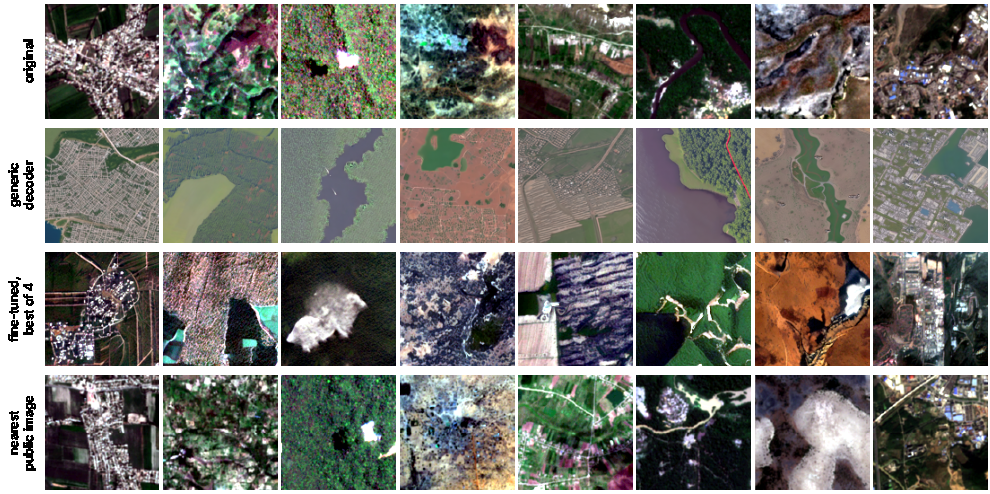
\includegraphics[width=\linewidth]{gen/fig_generic_ft.pdf}
\caption{The first eight attacked VertiBench test images (contrast-stretched for display, as the two bottom rows), the output of the generic decoder of Fig.~\ref{fig:generic}, the best of \giftNBest{} samples of the same decoder fine-tuned on public in-domain pairs, and the public image nearest to the upload in CLIP-L space, which is always of a training location.}\label{fig:generic-ft}
\end{figure}

\begin{figure}[tbp]
\centering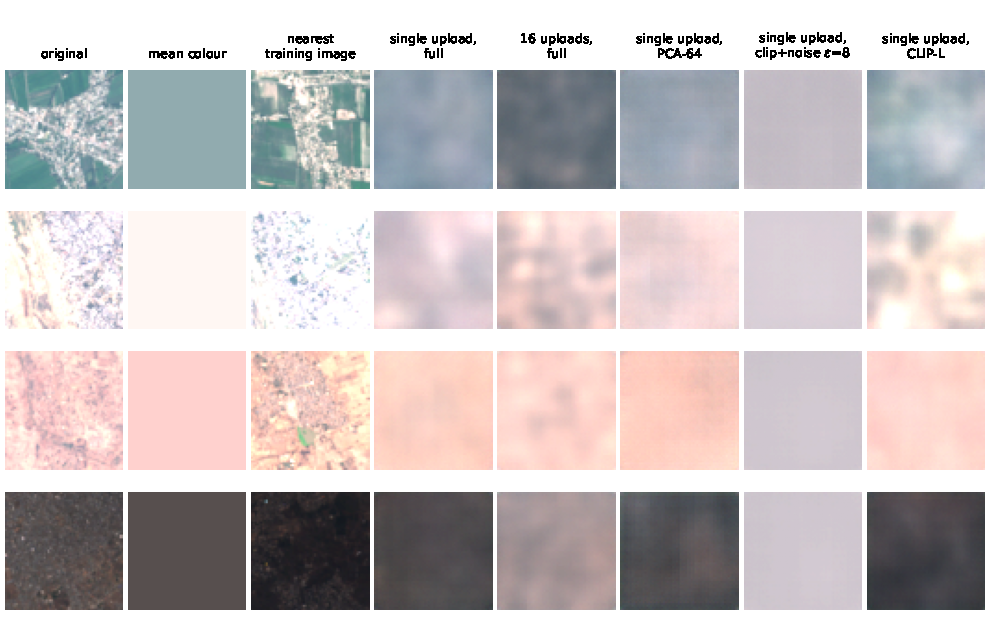
\includegraphics[width=\linewidth]{gen/fig_inversion.pdf}
\caption{Decoders trained on in-domain image--feature pairs, on held-out VertiBench test images ($64\times64$ RGB thumbnails, brightness $\times3$ for display). From left to right: original; its mean colour; nearest training image in DINOv2-g feature space; decoder output from one full DINOv2-g upload, from a PCA-64 upload, from a clipped noisy upload, and from one CLIP-L upload.}\label{fig:inversion}
\end{figure}

\begin{table}[tbp]
\caption{Utility versus leakage of the upload format on VertiBench (DINOv2-g, 224\,px). Accuracy on the test set (5 seeds); PSNR and SSIM of the single-upload inversion; re-identification (top-1, $16\times16$ thumbnails) of the source among the 12{,}560 test images and of its location among the \invNLoc{} test locations. Each value is that of the strongest attacker: the deconvolutional decoder trained for \invEpochs{} epochs, the same trained for \invShortEpochs{} epochs ($^{s}$) or the linear decoder ($^{\ell}$). Clip + noise: per-party Gaussian mechanism, per-upload $(\varepsilon, 10^{-5})$.}\label{tab:privacy}
\centering\scriptsize
\setlength{\tabcolsep}{3.5pt}
\begin{adjustbox}{max width=\linewidth}
\begin{tabular}{@{}lrccccc@{}}
\toprule
 & & & & & \multicolumn{2}{c@{}}{Re-id (\%)}\\\cmidrule(l){6-7}
Upload format & Upload & Acc. (\%) & PSNR (dB) & SSIM & image & location\\
\midrule
\inputtab{gen/tab_privacy.tex}
\bottomrule
\end{tabular}
\end{adjustbox}
\end{table}

\begin{table}[tbp]
\caption{Party-side transforms of the CLIP-L upload on VertiBench. Accuracy of the usual head on the 16 transformed uploads (3 seeds). Linkage: share of the \giVbNTest{} test uploads of a party whose embedding, mapped back to CLIP space from $k$ leaked image--upload pairs of that party ($k=0$: spectral alignment with public in-domain features), is closer to the true CLIP embedding of its image than to that of any other test image (chance \giVbChance\,\%). Raw uploads need no map: the public projection gives the embedding itself.}\label{tab:defences}
\centering\scriptsize
\setlength{\tabcolsep}{4pt}
\begin{tabular}{@{}lrcccccc@{}}
\toprule
& & & \multicolumn{5}{c@{}}{Linkage (\%) with $k$ leaked pairs}\\\cmidrule(l){4-8}
Transform & Dim. & Acc. (\%) & 0 & 10 & 100 & 1{,}000 & 3{,}142\\
\midrule
\inputtab{gen/tab_defences.tex}
\bottomrule
\end{tabular}
\end{table}

\FloatBarrier

\section{Reproducibility}\label{app:repro}

This appendix lists the code, data, compute and training details behind every result of the paper.

\paragraph{Code, data and compute.}
All code, configurations, raw result files and the scripts that generate every table, figure and quoted number from them are in the accompanying repository\footnote{\url{https://github.com/xavierxav/Simple-VFL}, directories \texttt{paper\_experiments} and \texttt{paper\_results}.}. All data sets are public. Each frozen head trains in seconds to minutes on one GPU; the whole study, including the end-to-end baselines, the image augmentation and the WorldStrat feature extraction, used about 110 Google Colab compute units on L4 and A100 GPUs.

\paragraph{Encoders and features.}
All encoders are used through their pooled output token at their native 224\,px input: DINOv2 ViT-S/B/L/g~\cite{oquab2024dinov2}, CLIP ViT-B/16 and ViT-L/14~\cite{radford2021clip}, SigLIP ViT-B/16~\cite{zhai2023siglip}, a supervised ImageNet ResNet-50 and a randomly initialised ViT-B; SSL4EO-S12 ViT-S/16~\cite{wang2023ssl4eo} on all 13 Sentinel-2 bands; BiomedCLIP~\cite{zhang2023biomedclip} and MONET~\cite{kim2024monet} for MILK10k. Satellite images are standardised per band with statistics of the released data (on WorldStrat, estimated on 200 random areas of all folds, without labels) and fed as RGB or as false-colour composites (B8-B4-B3, B12-B8A-B4) to expose the infrared bands to RGB encoders; the SPOT image is encoded at its own pixel count (1050, 518, 266 and 168\,px for 1.5, 3, 6 and 10\,m). Natural images use each model's own normalisation. Features are extracted once in half precision; a party holding several images of an entity (revisits, views) averages their features.

\paragraph{Heads.}
The reference head is a two-layer MLP ($Kd\to1000\to C$, batch normalisation, ReLU; 24.6\,M weights for 16 DINOv2-g parties, 3.1\,M for two). \emph{Late fusion} trains one MLP per party and averages their log-probabilities with a weight $w$ (chosen on the validation fold, or fixed to $\tfrac12$). A \emph{branch} head projects each party to 512 dimensions (linear, LayerNorm, GELU), classifies their concatenation, adds one auxiliary classifier per party (loss weight $\tfrac12$) and, with modality dropout, zeroes one random party in 30\,\% of the training samples. A \emph{pooling} head normalises each party's vector (LayerNorm), averages them over the parties present and applies the MLP; it requires all parties to share an encoder and feature space. A \emph{set} head applies one weight-shared MLP to each of the vectors of a party that holds several images and pools them by attention before the classifier. All heads on frozen features use Adam (learning rate $10^{-3}$, batch 512), at most 50 epochs, \texttt{ReduceLROnPlateau} and early stopping on the unweighted validation loss; the best validation checkpoint is tested (Table~\ref{tab:milkreg} checks two other stopping rules). On the imbalanced WorldStrat and MILK10k labels the loss is class-balanced and macro F1 is the primary metric.

\paragraph{Seeds, folds and tests.}
On VertiBench the public split is used as is (3{,}142 training and 785 test samples); 15\,\% of the training samples are held out for validation with the seed, so seeds change the initialisation and the validation subset, not the test set. We report mean\,$\pm$\,sample standard deviation over five seeds (VertiBench, unless noted), three seeds (CIFAR, ModelNet40; five for the protocol of Sun et al.) or five stratified cross-validation folds (WorldStrat, grouped by site; MILK10k, over lesions), where fold $f$ is the test set and fold $f{+}1$ the validation set. On the fixed VertiBench test set, comparisons use paired bootstrap intervals and exact McNemar tests on test predictions from seed-averaged probabilities (App.~\ref{app:audit}); WorldStrat and MILK10k comparisons are paired by fold. On MILK10k, the age imputation and standardisation of the metadata party are computed on all lesions, without labels.

\paragraph{Baselines.}
\emph{VertiBench recipe}: our re-implementation of the published SplitNN configuration (one ResNet-18 per party with a $9\times9$ stride-2 input convolution, MLP aggregation, Adam with learning rate $10^{-5}$, step decay, batch 32, 50 epochs, last epoch tested, 16 bottoms run sequentially) on the 13 bands. \emph{SplitNN, our recipe}: standard ResNet-18 bottoms~\cite{he2016resnet}, from scratch or ImageNet weights, and the same MLP top model as our head (Adam, one-cycle schedule, 40 epochs, batch 64, flips, best validation checkpoint). \emph{FedOnce}~\cite{wu2022fedonce}: every party trains a ResNet-18 on its unlabelled training images with Noise As Targets~\cite{bojanowski2017nat} (64-d targets, Hungarian re-assignment every 3 epochs, 100 epochs) or SimCLR~\cite{chen2020simclr} and uploads its output once; each party's encoder is pre-trained once and the five seeds re-train the head only, so the standard deviation of these rows is conditional on that pre-training. \emph{Same-backbone split learning}: frozen and LoRA-adapted CLIP ViT-B/16 bottoms on VertiBench; frozen, LoRA-adapted and (for DINOv2) fully fine-tuned CLIP ViT-B/16 and DINOv2 ViT-B/14 bottoms on MILK10k, with ResNet-18 baselines from scratch and from ImageNet weights. LoRA~\cite{hu2022lora} uses rank 16 on the attention query and value projections; the ViT runs use 10 epochs, augmentation and the best validation checkpoint, with a class-balanced loss on MILK10k. These baselines follow published or standard recipes without extensive hyper-parameter search.
.
% Every number is a macro of gen/macros.tex or a value quoted from the published papers.

\section{Full VertiBench results and encoders}\label{app:vb}

This appendix supports both contributions: it details the VertiBench baselines and the comparison of frozen encoders behind the foundation-model points of the frontier (C1), and shows how accuracy depends on the number of parties of this benchmark (C2).

\begin{table}[tbp]
\caption{VertiBench Satellite, all methods (16 parties, official test set). Upload: training payload per sample over all parties (activations or logits up, gradients down when needed). GFLOPs: party compute per image (a training run for split learning, one forward pass otherwise). Time: minutes on one A100 (split training, FedOnce pre-training or feature extraction). Mean\,$\pm$\,std over 5 seeds unless noted; --: not recorded.}\label{tab:main}
\centering\scriptsize
\setlength{\tabcolsep}{3pt}
\begin{adjustbox}{max width=\linewidth}
\begin{tabular}{@{}lcrrrccc@{}}
\toprule
Method & Bands & Upload & GFLOPs & Time & Acc. (\%) & F1 (\%) & AUC (\%)\\
\midrule
\inputtab{gen/tab_main.tex}
\bottomrule
\end{tabular}
\end{adjustbox}
\end{table}

\paragraph{Baselines.}
Our re-implementation of the published VertiBench split-learning configuration reaches $\reproAcc\pm\reproStd$\,\% on the 13 bands after its last epoch, in line with the published $81.2\pm0.4$\,\% (Table~\ref{tab:main}). Our own split-learning recipe is weaker from scratch (\splitAllAcc\,\% on 13 bands, \splitRGBAcc\,\% on RGB) and matches it from ImageNet weights (\splitPTAcc\,\% on RGB). FedOnce, whose parties learn their encoder on their own unlabelled images before a single upload, reaches \natAcc\,\% with Noise As Targets and \sslAllAcc\,\% with SimCLR: on 3{,}142 training locations, self-supervised training does not produce better features than supervised split learning. Macro F1 and AUC order the frozen foundation encoders above these baselines as accuracy does, but not among themselves (CLIP-B has the best macro F1 and a lower accuracy than CLIP-L). No difference between the two best encoders is detected: on the same test predictions (seed-averaged probabilities), CLIP-L leads DINOv2-g by $\pairDiff$ points, 95\,\% bootstrap interval $[\pairLo, \pairHi]$, McNemar $p=\pairP$.

\paragraph{Encoder choice.}
Table~\ref{tab:encoders} compares nine frozen encoders under the same head. All pre-trained ViTs lie between 81.6 and 85.2\,\%, a supervised ImageNet ResNet-50 reaches 80.9\,\%, and a randomly initialised ViT-B only 75.1\,\%: the gain comes from pre-training, not from the head. Size matters moderately: DINOv2 gains 2.4 points from ViT-S/14 (81.8\,\%) to ViT-g/14 (84.2\,\%), whereas CLIP ViT-B/16 is within one point of ViT-L/14. In FLOPs a large encoder is not cheaper than training a small bottom model: one DINOv2-g pass costs \vbGGF{} GFLOPs per image, more than the \rEighteenTrainGF{} GFLOPs of 50 training epochs of the VertiBench ResNet-18 bottom, whereas CLIP-B costs \vbClipBGF{} GFLOPs; encoding all images of the 16 parties takes \vbGMin{} minutes with DINOv2-g and \vbClipBMin{} with CLIP-B on one A100. Parties may also upload the features of two encoders side by side: CLIP-L with CLIP-B reaches \comboLB\,\%, DINOv2-g with CLIP-L \comboGL\,\%, a small gain for a larger upload. The encoder is therefore a parameter of the regime, chosen for cost.

\paragraph{Number of parties.}
The 16 VertiBench parties observe the same sensor at different dates and are largely redundant: with DINOv2-g, one party alone gives \soloMean\,\% on average (\soloMin--\soloMax), two parties \partiesKTwo\,\%, four \partiesKFour\,\%, eight \partiesKEight\,\% and all 16 \partiesKAll\,\% (Fig.~\ref{fig:parties}, left). This redundancy is a property of the benchmark: it limits what any method can gain by combining parties here, and it lets a suitable head tolerate missing parties (App.~\ref{app:pca}).

\begin{table}[tbp]
\caption{Frozen encoders on VertiBench (224\,px RGB, one upload, 5 seeds). Params in millions, GFLOPs per image, $d$ per party. Bottom: each party uploads two encoders' features side by side (features standardised).}\label{tab:encoders}
\centering\scriptsize
\setlength{\tabcolsep}{3.5pt}
\begin{adjustbox}{max width=\linewidth}
\begin{tabular}{@{}lrrrccc@{}}
\toprule
Encoder & Params & GFLOPs & $d$ & Acc. (\%) & F1 (\%) & Linear acc. (\%)\\
\midrule
\inputtab{gen/tab_encoders.tex}
\midrule
\multicolumn{7}{@{}l}{\emph{Each party uploads two encoders' features (standardised)}}\\
\inputtab{gen/tab_combo_enc.tex}
\bottomrule
\end{tabular}
\end{adjustbox}
\end{table}

\begin{figure}[tbp]
\centering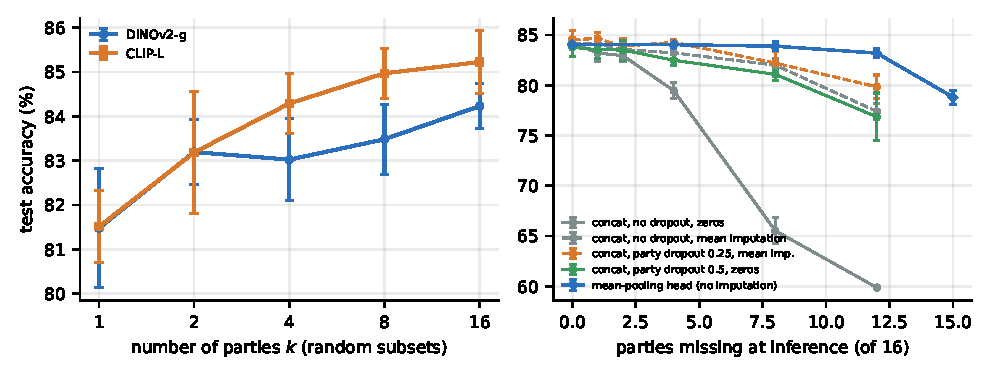
\includegraphics[width=\linewidth]{gen/fig_parties.pdf}
\caption{VertiBench, DINOv2-g. Left: accuracy with $k$ randomly chosen parties (3 subsets $\times$ 5 seeds). Right: parties missing at inference for a concatenation head (missing uploads replaced by zeros or by the party's training mean, with and without party dropout during training) and for a head that averages per-party embeddings.}\label{fig:parties}
\end{figure}

\FloatBarrier

\section{Compression grid}\label{app:pca}

This appendix supports contribution C1: it gives the full grid of local PCA and quantisation from which the main text takes the knee of the frontier, and the limits of compressing without coordination.

\paragraph{Protocol.}
Because the encoder is frozen, each party can fit a PCA on its own training features (keeping $d'\le d$ components; the basis stays with the party) and quantise every coordinate uniformly to $b$ bits between its 1st and 99th training percentiles. The label owner trains the head on the de-quantised values. No labels, shared basis or coordination are needed, but the samples must still be aligned across parties; the few hundred bytes of quantiser bounds that each party sends once are not counted.

\paragraph{Selection under a byte budget.}
On frozen DINOv2-g features we run the grid of Table~\ref{tab:pareto} (16 to 512 components or no PCA, 1 to 16 bits) and select, under each budget, the configuration with the best \emph{validation} accuracy (Fig.~\ref{fig:pareto}). For the 16 parties together, 256\,B per sample (\selTwoCfg) give \selTwoAcc\,\%, 512\,B (\selFiveCfg) \selFiveAcc\,\%, 2\,KiB (\selTwokCfg) \selTwokAcc\,\%, and the full budget selects \selFullCfg{} (\selFullBytes) at \selFullAcc\,\%, against \fullAcc\,\% for the uncompressed 48\,KiB. Moderate compression therefore costs nothing on this benchmark; with 4 bits or more, the PCA-256 and PCA-512 rows are even slightly above the uncompressed features, which we attribute, without having tested it, to a regularising effect on the small labelled set. Even one bit per feature keeps \cmpOneBit\,\%.

\paragraph{Other benchmarks.}
Compression is not free everywhere. On MILK10k a per-party PCA-256 slightly lowers the macro F1 of the concatenation head (\mrGPca, \mrCPca{} and \mrMPca\,\% against \mrGCat, \mrCCat{} and \mrMCat\,\% with DINOv2-g, CLIP-L and MONET; Table~\ref{tab:milkreg}). On WorldStrat, PCA-256 per party changes IPCC and LCCS F1 by \wpIpccPca{} and \wpLccsPca{} points relative to concatenation of the same inputs (Table~\ref{tab:wsfusion}).

\paragraph{Missing parties.}
A concatenation head breaks when parties are missing at inference and their uploads are replaced by zeros (\missZeroEightZ\,\% with 8 of 16 missing, \missZeroTwelveZ\,\% with 12); imputing the party's training mean (\missZeroTwelveM\,\% with 12 missing) or training with party dropout 0.5 (\missHTwelveZ\,\%) repairs most of it (Fig.~\ref{fig:parties}, right). A pooling head (App.~\ref{app:repro}) needs neither: it reaches \poolGMean\,\% with all parties, \poolMissTwelve\,\% with 12 missing and still \poolMissFifteen\,\% with a single party left. It requires a shared feature space, however, and uncoordinated compression removes it: after per-party PCA-64, whose bases differ between parties, the pooling head drops to \poolGPcaMean\,\%, while concatenation of the same uploads keeps \poolGPcaConcat\,\%. Nor does it apply to parties with different modalities or encoders. Local compression and robustness to missing parties must thus be traded off, unless the parties agree on a common basis (e.g.\ one fitted on public images; not tested).

\begin{figure}[tbp]
\centering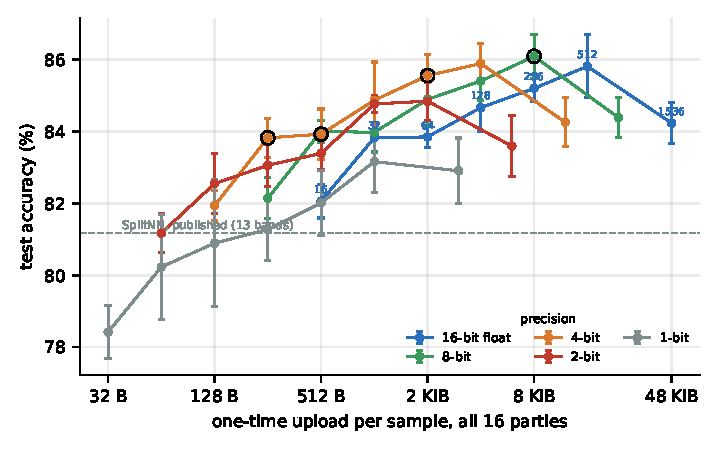
\includegraphics[width=0.78\linewidth]{gen/fig_pareto.pdf}
\caption{VertiBench: accuracy versus one-time upload (bytes per sample, 16 parties) for per-party PCA (number of components annotated on the 16-bit curve) and uniform scalar quantisation of frozen DINOv2-g features, MLP head, 5 seeds. Circles: configuration with the best \emph{validation} accuracy under a budget of 256\,B, 512\,B, 2\,KiB and 48\,KiB.}\label{fig:pareto}
\end{figure}

\begin{table}[tbp]
\caption{The compression grid of Fig.~\ref{fig:pareto} (VertiBench, DINOv2-g, MLP head, 5 seeds). $d'$: PCA components per party (1536: no PCA); $b$: bits per coordinate; upload: one-time payload per sample over the 16 parties. Validation accuracy (seed mean) is the selection criterion; test accuracy and AUC are mean\,$\pm$\,std.}\label{tab:pareto}
\centering\scriptsize
\setlength{\tabcolsep}{4pt}
\begin{tabular}{@{}rrrccc@{}}
\toprule
$d'$ & $b$ & Upload & Val.\ acc.\ (\%) & Test acc.\ (\%) & AUC (\%)\\
\midrule
\inputtab{gen/tab_pareto.tex}
\bottomrule
\end{tabular}
\end{table}

\FloatBarrier

\section{VertiBench audit}\label{app:audit}

This appendix supports contribution C2: it details the audit of the official VertiBench Satellite split and the paired tests behind the comparisons with SplitNN in the main text.

\paragraph{Mapping to source areas.}
Image fingerprints match \auMapTrain{} training and \auMapTest{} test samples to distinct WorldStrat areas (5th-percentile correlation \auScore); \auMapOverlap{} areas appear in both splits.

\paragraph{Siblings, confounded with class.}
The split is not grouped by site, however: \auSibN{} test samples (\auSibShare\,\%) have a training tile from the same site, all from the two sources whose sites are cut into $3\times3$ tiles. They account for \auSibN{} of the 113 test samples in classes 0 and 1, so the \auNoSibN{} test samples without a known sibling are almost all of classes 2 and 3, and class and sibling effects cannot be separated. Table~\ref{tab:audit} gives each head's accuracy on the two subsets. SplitNN is markedly more accurate with siblings (\auSnSib{} vs.\ \auSnNoSib\,\%); the one-shot heads are similarly accurate on both (CLIP-L: \auClipSib{} vs.\ \auClipNoSib\,\%), and the four-logit CLIP heads and frozen split learning are \emph{less} accurate with siblings. The margins over SplitNN are therefore larger on the subset without siblings.

\paragraph{Paired tests.}
The three-seed SplitNN re-run that retains test probabilities averages \auSnAll\,\% accuracy, versus \reproAcc\,\% over five seeds in Table~\ref{tab:main}. We pair test predictions after averaging probabilities over the same three seeds per method (exact McNemar test and 95\,\% paired bootstrap interval, 10{,}000 resamples). On the whole test set, the two CLIP one-shot MLPs, the three four-logit heads and CLIP-B split learning with LoRA beat SplitNN at the 5\,\% level; DINOv2-g's one-shot MLP ($+\pairSnGDiff$ points, $p\pairSnGP$) and frozen CLIP-B split learning do not (Table~\ref{tab:audit}). In detail, the CLIP-L, CLIP-B and DINOv2-g one-shot heads gain $\pairSnClipDiff$ ($p\pairSnClipP$), $\pairSnClipBDiff$ ($p\pairSnClipBP$) and $\pairSnGDiff$ points ($p\pairSnGP$); the CLIP-L, DINOv2-g and CLIP-B four-logit heads give $p\pairSnLgClipP$, $p\pairSnLgGP$ and $p\pairSnLgClipBP$, LoRA split learning $p\pairSnLoraP$ and frozen split learning $p\pairSnSplitFrozenP$. Without known siblings every margin grows and all are significant (CLIP-L: $\pairSnClipNoSibDiff$ points, $p\pairSnClipNoSibP$). These $p$-values are uncorrected: after a Holm correction over the \holmN{} comparisons, \holmSurvive{} remain below 0.05, LoRA split learning and the CLIP-B four-logit head. LoRA itself is unstable across seeds (\seedLoraMin{} to \seedLoraMax\,\%); paired with the ensemble of the one-shot CLIP-B head on the same seeds, its lead is $\pairLoraHeadDiff$ points ($[\pairLoraHeadLo,\pairLoraHeadHi]$, $p\pairLoraHeadP$).

\paragraph{Nearest public image.}
The retrieval attacker of App.~\ref{app:privacy} does not owe its success to siblings: across test uploads, the label of the nearest public training image in CLIP-L space matches in \nnPubAll\,\% of the cases (\nnPubSib\,\% with known siblings, \nnPubNoSib\,\% without), and the neighbour is itself a sibling in just \nnPubIsSib\,\% of the sibling cases, about 5\,\% overall.

\begin{table}[tbp]
\caption{VertiBench audit. Test accuracy (\%) on all 785 test samples, on the \auSibN{} with a training tile from the same site and on the \auNoSibN{} without; paired gain over SplitNN in points with 95\,\% paired bootstrap interval and exact McNemar test, on all samples and without siblings. Probabilities averaged over 3 seeds per method.}\label{tab:audit}
\centering\scriptsize
\setlength{\tabcolsep}{3pt}
\begin{adjustbox}{max width=\linewidth}
\begin{tabular}{@{}lccccccc@{}}
\toprule
& \multicolumn{3}{c}{Accuracy (\%)} & \multicolumn{2}{c}{Gain over SplitNN, all} & \multicolumn{2}{c@{}}{Gain, no sibling}\\
\cmidrule(lr){2-4}\cmidrule(lr){5-6}\cmidrule(l){7-8}
Head & all & sibling & no sibling & points [95\,\% CI] & McNemar & points [95\,\% CI] & McNemar\\
\midrule
SplitNN, VertiBench recipe & \auSnAll & \auSnSib & \auSnNoSib & -- & -- & -- & --\\
\midrule
One-shot MLP, CLIP-L & \auClipAll & \auClipSib & \auClipNoSib & $\pairSnClipDiff$ $[\pairSnClipLo,\pairSnClipHi]$ & $p\pairSnClipP$ & $\pairSnClipNoSibDiff$ $[\pairSnClipNoSibLo,\pairSnClipNoSibHi]$ & $p\pairSnClipNoSibP$\\
One-shot MLP, CLIP-B & \auClipBAll & \auClipBSib & \auClipBNoSib & $\pairSnClipBDiff$ $[\pairSnClipBLo,\pairSnClipBHi]$ & $p\pairSnClipBP$ & $\pairSnClipBNoSibDiff$ $[\pairSnClipBNoSibLo,\pairSnClipBNoSibHi]$ & $p\pairSnClipBNoSibP$\\
One-shot MLP, DINOv2-g & \auGAll & \auGSib & \auGNoSib & $\pairSnGDiff$ $[\pairSnGLo,\pairSnGHi]$ & $p\pairSnGP$ & $\pairSnGNoSibDiff$ $[\pairSnGNoSibLo,\pairSnGNoSibHi]$ & $p\pairSnGNoSibP$\\
\midrule
Four-logit head, CLIP-L & \auLgClipAll & \auLgClipSib & \auLgClipNoSib & $\pairSnLgClipDiff$ $[\pairSnLgClipLo,\pairSnLgClipHi]$ & $p\pairSnLgClipP$ & $\pairSnLgClipNoSibDiff$ $[\pairSnLgClipNoSibLo,\pairSnLgClipNoSibHi]$ & $p\pairSnLgClipNoSibP$\\
Four-logit head, CLIP-B & \auLgClipBAll & \auLgClipBSib & \auLgClipBNoSib & $\pairSnLgClipBDiff$ $[\pairSnLgClipBLo,\pairSnLgClipBHi]$ & $p\pairSnLgClipBP$ & $\pairSnLgClipBNoSibDiff$ $[\pairSnLgClipBNoSibLo,\pairSnLgClipBNoSibHi]$ & $p\pairSnLgClipBNoSibP$\\
Four-logit head, DINOv2-g & \auLgGAll & \auLgGSib & \auLgGNoSib & $\pairSnLgGDiff$ $[\pairSnLgGLo,\pairSnLgGHi]$ & $p\pairSnLgGP$ & $\pairSnLgGNoSibDiff$ $[\pairSnLgGNoSibLo,\pairSnLgGNoSibHi]$ & $p\pairSnLgGNoSibP$\\
\midrule
Split learning, CLIP-B frozen & \auSplitFrozenAll & \auSplitFrozenSib & \auSplitFrozenNoSib & $\pairSnSplitFrozenDiff$ $[\pairSnSplitFrozenLo,\pairSnSplitFrozenHi]$ & $p\pairSnSplitFrozenP$ & $\pairSnSplitFrozenNoSibDiff$ $[\pairSnSplitFrozenNoSibLo,\pairSnSplitFrozenNoSibHi]$ & $p\pairSnSplitFrozenNoSibP$\\
Split learning, CLIP-B LoRA & \auLoraAll & \auLoraSib & \auLoraNoSib & $\pairSnLoraDiff$ $[\pairSnLoraLo,\pairSnLoraHi]$ & $p\pairSnLoraP$ & $\pairSnLoraNoSibDiff$ $[\pairSnLoraNoSibLo,\pairSnLoraNoSibHi]$ & $p\pairSnLoraNoSibP$\\
\bottomrule
\end{tabular}
\end{adjustbox}
\end{table}

\FloatBarrier

\section{MILK10k details}\label{app:milk}

This appendix supports contribution C1: it gives the party combinations, fusion heads and regularisation checks behind the frozen MILK10k rows of Table~\ref{tab:freeze}, and the same-recipe comparison of frozen and adapted backbones. Figure~\ref{fig:frontier-axes-milk} places the MILK10k points on the other axes of the cost accounting: one-shot points need \frMilkRoundsMatch{} message against \frMilkRoundsSplitNN{} for ResNet-18 split learning, and \frMilkGflopsMatchName{} exceeds that baseline (\frMilkGflopsMatchAcc{} vs.\ \frMilkBestNonFound\,\%) with \frMilkGflopsRatio{} times less party compute.

\begin{figure}[t]
\centering\IfFileExists{gen/fig_frontier_axes_milk.pdf}{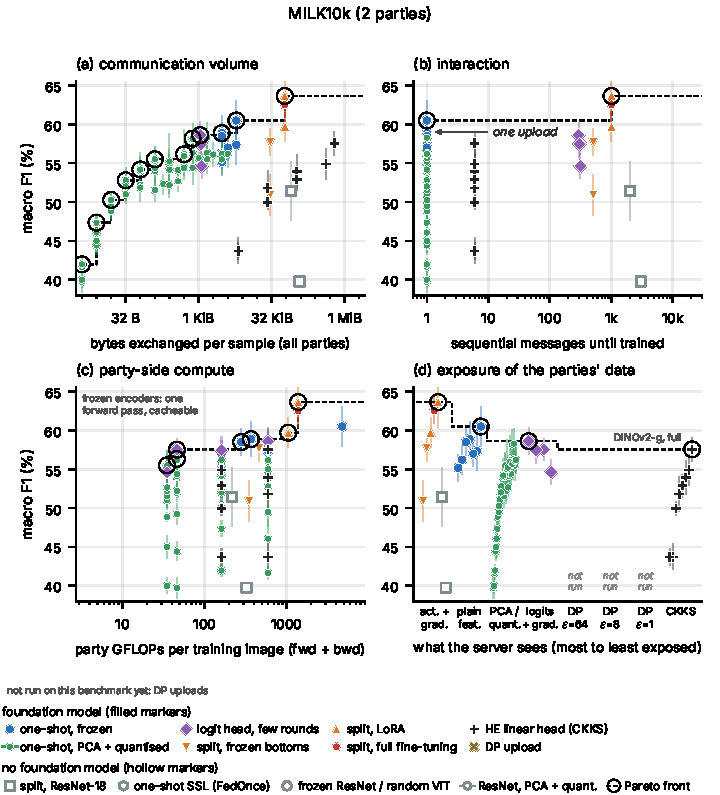
\includegraphics[width=\linewidth]{gen/fig_frontier_axes_milk.pdf}}{\fbox{\parbox{0.9\linewidth}{\centering fig\_frontier\_axes\_milk pending}}}
\caption{MILK10k along the axes of Fig.~\ref{fig:frontier-axes}: (a)~bytes per training sample, (b)~sequential messages until trained, (c)~party GFLOPs per training image (forward and backward), (d)~exposure ladder. Only DP is marked as not run. Circled: Pareto-optimal points.}\label{fig:frontier-axes-milk}
\end{figure}

\begin{table}[tbp]
\caption{MILK10k, all methods (2 parties, 5 folds, class-balanced loss). Split learning trains the bottoms with the server's gradients; one-shot rows use frozen features and an MLP head (concatenation, or late fusion on features averaged over 8 rotations and flips). Upload per training sample: over all training epochs for split learning (30 for ResNet-18 from scratch, 20 from ImageNet, 10 for ViTs), once for one-shot. Time: minutes per fold (one-shot: encoding, estimated).}\label{tab:freeze}
\centering\scriptsize
\setlength{\tabcolsep}{3pt}
\begin{adjustbox}{max width=\linewidth}
\begin{tabular}{@{}llrrrccc@{}}
\toprule
Party models & Training & Trainable & Upload & Time & F1 (\%) & Bal.\ acc.\ (\%) & Acc.\ (\%)\\
\midrule
\inputtab{gen/tab_freeze.tex}
\bottomrule
\end{tabular}
\end{adjustbox}
\end{table}

\paragraph{Real modalities complement each other little.}
The dermoscopic image alone gives \milkGDerm\,\% macro F1 with DINOv2-g, the clinical photograph \milkGClin\,\%, the metadata \milkMeta\,\% (Table~\ref{tab:milk}). Concatenating the two images adds less than one point over the dermoscopy (\milkGBoth\,\%), three points with CLIP-L (\milkCDerm{} $\to$ \milkCBoth\,\%); the metadata add at most one point on top. The general-purpose encoders match or beat the medical ones (BiomedCLIP, MONET). Splitting the dermoscopy into two halves, as split benchmarks do, \emph{loses} information instead: \milkGHalves\,\% against \milkGDerm\,\% for the whole image, because each party's encoder sees half a lesion. Two caveats apply to all MILK10k numbers: folds are drawn over lesions, as the release has no patient identifiers, and each test fold holds only 40 to 61 lesions of the two rarest classes.

\paragraph{How the parties are combined matters as much as the encoder.}
A concatenation MLP under-uses the weaker party. Training one head per party and averaging their log-probabilities (late fusion) is better for every encoder (Table~\ref{tab:milkfusion}): \mfGLate\,\% instead of \mfGCat\,\% with DINOv2-g, \mfCLate\,\% instead of \mfCCat\,\% with CLIP-L, \mfGMLate\,\% when each party uploads DINOv2-g and MONET features; with DINOv2-g, the two parties together then reach \mfGLate\,\%, about three points more than the dermoscopic party alone (\milkGDerm\,\%). Late fusion also suits VFL: each party's head can be trained, audited and dropped independently. The gain is bounded by the data: \mfGBoth\,\% of the lesions are misclassified by both single-party heads, against \mfGIndep\,\% if their errors were independent---the two modalities fail on the same, intrinsically hard lesions.

\paragraph{Over-fitting or modality competition?}
With 3{,}100 training lesions and 2--3k input dimensions, the concatenation head could simply over-fit. Three observations speak against this being the main cause (Table~\ref{tab:milkreg}). First, regularising it---input dropout, Gaussian feature noise, feature mixup, a per-party PCA---gains at most one point and never reaches late fusion. Second, late fusion does not need its tuned weight: a fixed weight of 0.5 does as well (\mrGLateHalf\,\% with DINOv2-g); paired by fold, it beats concatenation by \mrGPairD\,$\pm$\,\mrGPairS{} points with DINOv2-g (\mrGPairW{} folds out of 5), \mrCPairD\,$\pm$\,\mrCPairS{} with CLIP-L (\mrCPairW/5) and \mrMPairD\,$\pm$\,\mrMPairS{} with MONET (\mrMPairW/5). Third, its advantage does not shrink with more data, as over-fitting would predict: it grows from 25\,\% to 100\,\% of the training folds for CLIP-L and MONET. Nor is it an artefact of our early-stopping rule on the unweighted validation loss: when both heads stop on the class-weighted validation loss or on the validation macro F1, late fusion still wins by \mrStopMin{} to \mrStopMax{} points over \mrStopN{} comparisons (DINOv2-g, CLIP-L, DINOv2-B, CLIP-B; stopping on the weighted loss lowers every head by up to \mrWlossDropMax{} points), and weight decay on the concatenation head leaves a gap of \mrWdMin{} to \mrWdMax{} points. The pattern rather matches the \emph{modality competition} documented for jointly trained multimodal networks~\cite{wang2020makes,huang2022modality,peng2022balanced}: a joint head learns the dominant dermoscopy first and stops before exploiting the clinical photograph, whereas separate heads must each use their own modality fully; the validation-tuned late fusion gives the weaker clinical party a weight of 0.3 to 0.5. Augmentation helps in image space, not in feature space: the parties can encode the 8 rotations and flips of each photograph once (8 times the encoding cost) and upload the mean, which raises late fusion to \mrGLateViews\,\% (DINOv2-g), \mrMLateViews\,\% (MONET), \fzViewsB\,\% (DINOv2-B) and \fzViewsCb\,\% (CLIP-B) at no extra communication. With CLIP-L it helps late fusion little (\mrCLateViews\,\%); there the best head is the concatenation trained on one of the 8 uploaded views per epoch (\mrCCatSampled\,\%, at 8 times the upload).

\paragraph{Frozen versus adapted under the same recipe.}
The frozen and adapted rows of Table~\ref{tab:freeze} differ in more than freezing (augmentation, head, standardisation, optimiser and schedule). In a paired re-run we therefore use the same split-learning recipe with frozen and LoRA bottoms. For DINOv2-B this gives \srFrozenB\,\% macro F1 frozen versus \srLoraB\,\% with LoRA (paired gain $\srGapB\pm\srGapSdB$ points, \srWinsB/5 folds); for CLIP-B, \srFrozenCb\,\% versus \srLoraCb\,\% ($\srGapCb\pm\srGapSdCb$ points, \srWinsCb/5 folds). Relative to the one-shot MLPs, freezing under the split recipe shifts F1 by $\srVsHeadB$ and $\srVsHeadCb$ points, respectively, so the larger same-recipe LoRA gain for CLIP-B partly reflects its weaker frozen baseline under that recipe. Adaptation wins on MILK10k under both recipes.

\begin{table}[tbp]
\caption{MILK10k: macro F1 (\%) of one-shot heads on frozen features for every combination of parties (5 folds, class-balanced MLP head). Bottom: the usual practice of splitting one image into a left and a right party.}\label{tab:milk}
\centering\scriptsize
\setlength{\tabcolsep}{3.5pt}
\begin{adjustbox}{max width=\linewidth}
\begin{tabular}{@{}lcccc@{}}
\toprule
Parties & \inputtab{gen/tab_milk_head.tex}\\
\midrule
\inputtab{gen/tab_milk.tex}
\bottomrule
\end{tabular}
\end{adjustbox}
\end{table}

\begin{table}[tbp]
\caption{MILK10k: how the label owner combines the clinical (A) and dermoscopic (B) uploads (macro F1, \%, 5 folds). Late fusion: one head per party, log-probabilities averaged with a weight chosen on the validation fold. Branches: per-party projection, auxiliary per-party losses and modality dropout (0.3). Last column: share of test lesions misclassified by both single-party heads, and (in brackets) what it would be if their errors were independent.}\label{tab:milkfusion}
\centering\scriptsize
\setlength{\tabcolsep}{3pt}
\begin{adjustbox}{max width=\linewidth}
\begin{tabular}{@{}lcccccc@{}}
\toprule
Encoder & B alone & A+B concat & A+B late fusion & A+B branches & A+B+C branches & Both wrong (\%)\\
\midrule
\inputtab{gen/tab_milkfusion.tex}
\bottomrule
\end{tabular}
\end{adjustbox}
\end{table}

\begin{table}[tbp]
\caption{MILK10k, clinical + dermoscopic parties: is the concatenation head over-fitting? Macro F1 (\%, 5 folds). Top: regularising the concatenation head versus late fusion. Middle: augmentation precomputed once by the parties (8 rotations and flips of each photograph). Bottom: gap between late fusion (fixed weight) and concatenation when the training folds are subsampled, and under other early-stopping rules than the unweighted validation loss.}\label{tab:milkreg}
\centering\scriptsize
\setlength{\tabcolsep}{3.5pt}
\begin{adjustbox}{max width=\linewidth}
\begin{tabular}{@{}lccc@{}}
\toprule
Head & DINOv2-g & CLIP-L & MONET\\
\midrule
\inputtab{gen/tab_milkreg.tex}
\bottomrule
\end{tabular}
\end{adjustbox}
\end{table}

\FloatBarrier

\section{WorldStrat: two sensors}\label{app:ws}

This appendix supports contribution C2: it reports a third natural partition, with genuinely different sensors, on which the two parties complement each other little once the folds are grouped by site.

\paragraph{Task.}
From the WorldStrat release~\cite{cornebise2022worldstrat} we build a two-party task on its \wsIpccN{} usable areas of $1.58\times1.58$\,km: party A holds the SPOT 6/7 pan-sharpened image (RGB, 1.5\,m, $1050\times1050$ pixels), party B the 16 Sentinel-2 L1C revisits (13 bands, 10\,m). The label owner holds one of three labels of the release metadata, all read at the centre of the area: the LCCS land-cover class of the 300\,m pixel of a global land-cover map~\cite{esa2017cci} (the 18 classes with at least 40 areas), its coarser IPCC category (7 classes), and the degree of urbanisation of the 1\,km SMOD cell (8 classes, from rural very-low-density to urban centre~\cite{pesaresi2019ghsl}). A label therefore describes only the centre of the image (4\,\% of its area for LCCS and IPCC); the parties also encode centre crops of 336\,m and 1\,km. To vary the information held by A, its image is degraded to 3, 6 and 10\,m before encoding, or cut into 16 full-resolution tiles of 262\,px whose features are averaged. Party B encodes every revisit as three composites (RGB, near- and short-wave infrared) and uploads, per composite, the mean over the 16 revisits or over the 8 least cloudy ones (ranked by a locally computed cloud score), possibly with the temporal standard deviation; for a set head it uploads all 16 vectors. The loss is class-balanced and macro F1 is the metric.

\paragraph{Grouped cross-validation.}
The five folds are stratified and grouped by site: all nine tiles of a site stay in the same fold. Stratification alone split sibling tiles across training and test and gave macro F1 about 6 to 9 points higher on the two land-cover tasks---the same leakage as in the official VertiBench split, which is built from the same areas (App.~\ref{app:audit}). All results below are site-grouped and paired by fold.

\paragraph{The second sensor adds little.}
Alone, the 1.5\,m SPOT image scores \wsIpccSpot{} against \wsIpccSms\,\% macro F1 for the Sentinel-2 revisits (RGB, NIR, SWIR) on IPCC, \wsLccsSpot{} against \wsLccsSms\,\% on LCCS and \wsSmodSpot{} against \wsSmodSms\,\% on SMOD (Table~\ref{tab:ws}). Their concatenation reaches \wsIpccFus, \wsLccsFus{} and \wsSmodFus\,\%: relative to SPOT, F1 changes by \wgIpccA{} points on IPCC (\wgIpccAW{} folds improve), \wgLccsA{} on LCCS (\wgLccsAW) and \wgSmodA{} on SMOD (\wgSmodAW). With DINOv2-g, the pair is thus at most a couple of points above the better single sensor on land cover, and below SPOT alone on urbanisation. The second sensor matters more when the first is weakened (Fig.~\ref{fig:ws}): at 3\,m, fusion adds \wgIpccThree{} points on IPCC (\wgIpccThreeW) and \wgLccsThree{} on LCCS (\wgLccsThreeW); at 10\,m, \wgIpccTen{} (\wgIpccTenW) and \wgLccsTen{} (\wgLccsTenW), whereas SMOD never gains (\wgSmodTen{} at 10\,m, \wgSmodTenW). For land cover, SPOT improves alone at 3\,m (\wsIpccSpotThree{} and \wsLccsSpotThree\,\%) or by averaging the features of 16 full-resolution tiles (\wfIpccSpotTiles{} and \wfLccsSpotTiles\,\%), rather than feeding DINOv2 the whole 1{,}050\,px image; adding the clearest revisits to the tiles yields \wpIpccTilesFus{} and \wpLccsTilesFus{} points (\wpIpccTilesFusW{} and \wpLccsTilesFusW). Adding infrared to RGB helps LCCS at native resolution and both land-cover labels at 10\,m. With a multispectral encoder (SSL4EO-S12 on the 13 bands) for party B, or CLIP-L for both parties, fused IPCC scores and their gain over the single sensors are larger (Table~\ref{tab:ws}), while SMOD barely changes; we did not test these rows in pairs. For native-resolution fusion, pooled out-of-fold per-class F1 gains over SPOT are largest for \wcIpccTop{} on IPCC and \wcLccsTop{} on LCCS (points and number of areas); F1 falls in \wcIpccNeg{} IPCC and \wcLccsNeg{} LCCS classes.

\paragraph{Why a second sensor adds little.}
The parties fail on the same areas: on IPCC both are wrong on \wfIpccBoth\,\% of them, nearly three times the \wfIpccIndep\,\% expected from independent errors, although an oracle choosing the right party would reach \wfIpccOracle\,\% accuracy. Context matters more than a second view of the labelled pixel: although labels are read at the centre of the area, the whole 1.58\,km SPOT image beats a 336\,m centre crop by \wpIpccCentre, \wpLccsCentre{} and \wpSmodCentre{} points (\wpIpccCentreW, \wpLccsCentreW{} and \wpSmodCentreW{} folds); with a 1\,km crop, land-cover scores are roughly unchanged and only SMOD still loses ground (\wfSmodSpotCk{} vs.\ \wfSmodSpot\,\%).

\paragraph{Fusion heads do not change the picture.}
No fusion variant of Table~\ref{tab:wsfusion} improves on plain-mean concatenation across all three labels. The set head over the 16 revisits changes F1 by \wpLccsSetCat{} to \wpIpccSetCat{} points while multiplying the Sentinel-2 payload by 16. Late fusion changes IPCC, LCCS and SMOD F1 by \wpIpccLateMean, \wpLccsLateMean{} and \wpSmodLateMean{} points with the plain mean (SMOD improves in \wpSmodLateMeanW{} folds), and by \wpIpccLateCat, \wpLccsLateCat{} and \wpSmodLateCat{} with the clearest-revisit summary, where the branch head trails concatenation by \wpIpccBranch, \wpLccsBranch{} and \wpSmodBranch{} points. Adding temporal standard deviations shifts the IPCC F1 of Sentinel-2 alone by \wpIpccStdSolo{} points (\wpIpccStdSoloW{} folds improve), and adding a centre crop to SPOT alone changes IPCC and LCCS by \wpIpccFC{} and \wpLccsFC{} points.

\begin{table}[tbp]
\caption{WorldStrat, 5 site-grouped folds: macro F1 (\%, mean\,$\pm$\,std) of each sensor alone and of their concatenation (MLP head; DINOv2-g unless noted). A: SPOT image; B: mean of the 16 Sentinel-2 revisits, encoded as RGB, as three composites (RGB, NIR, SWIR) or on all 13 bands by SSL4EO-S12. Note the column order.}\label{tab:ws}
\centering\scriptsize
\setlength{\tabcolsep}{4pt}
\begin{tabular}{@{}lccc@{}}
\toprule
Parties & IPCC & SMOD & LCCS\\
\midrule
\inputtab{gen/tab_ws.tex}
\bottomrule
\end{tabular}
\end{table}

\begin{figure}[tbp]
\centering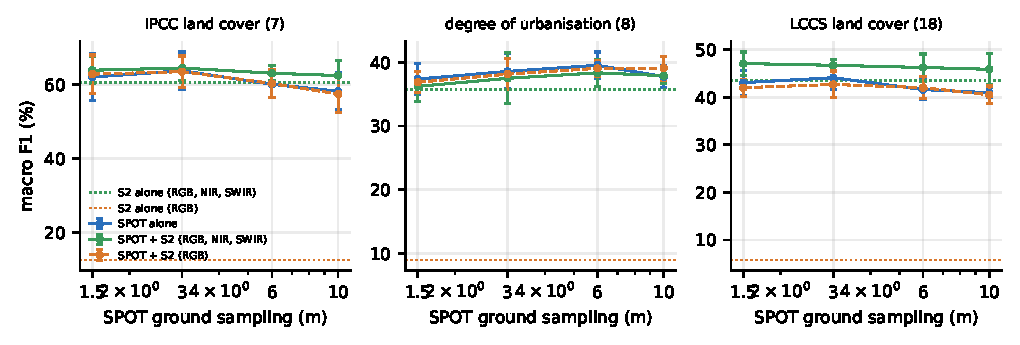
\includegraphics[width=\linewidth]{gen/fig_ws.pdf}
\caption{WorldStrat: macro F1 (mean over 5 site-grouped folds, DINOv2-g, MLP head) of the SPOT party alone and with the Sentinel-2 party, as the SPOT image is degraded from 1.5 to 10\,m. Dotted: Sentinel-2 alone. Fold standard deviations are about 1 to 6 points; paired differences are given in the text.}\label{fig:ws}
\end{figure}

\begin{table}[tbp]
\caption{WorldStrat: single parties and fusion heads (macro F1, \%, mean\,$\pm$\,std over 5 site-grouped folds, DINOv2-g). S2 vectors: number of 4{,}608-d vectors (RGB, NIR and SWIR composites) the Sentinel-2 party uploads per area; the SPOT party uploads one 1{,}536-d vector (two with the centre crop, three with three scales). C: whole SPOT image and mean of the 8 least cloudy revisits. All variants remain one-shot.}\label{tab:wsfusion}
\centering\scriptsize
\setlength{\tabcolsep}{3pt}
\begin{adjustbox}{max width=\linewidth}
\begin{tabular}{@{}lcccc@{}}
\toprule
Configuration & S2 vectors & IPCC & LCCS & SMOD\\
\midrule
\inputtab{gen/tab_wsfusion.tex}
\bottomrule
\end{tabular}
\end{adjustbox}
\end{table}

\FloatBarrier

\section{Classic split benchmarks}\label{app:classic}

This appendix supports contribution C2 by showing why natural benchmarks are needed: on the classic CIFAR and ModelNet40 splits, the gains of a single upload of frozen features mostly measure pre-training.

\paragraph{Splits.}
CIFAR-10/100~\cite{krizhevsky2009cifar} are split as in the papers we compare with: top/bottom halves ($K=2$) and $16\times16$ quadrants ($K=4$) as in VFLAIR~\cite{zou2024vflair} and FedOnce~\cite{wu2022fedonce}, and left/right halves with only $N_o\in\{256,\dots,2048\}$ aligned labelled samples as in Sun et al.~\cite{sun2023oneshotvfl}. Halves are upsampled by 7 ($16\times32\to112\times224$) and quadrants by 14 ($16\times16\to224\times224$), so four quadrants are encoded with four times as many tokens as two halves ($4\times256$ against $2\times128$). ModelNet40~\cite{wu2015modelnet} uses 12 rendered views per object~\cite{su2015mvcnn} (9{,}843 training and 2{,}468 test objects), one view per party ($K=12$) or three per party ($K=4$). We quote the published numbers of the original papers, including VIMADMM~\cite{xie2024vimadmm}.

\paragraph{Large gains that mostly measure pre-training.}
Frozen DINOv2-g features beat every published number by a wide margin (Table~\ref{tab:classic}): \cTenGTwo\,\% on CIFAR-10 cut into top and bottom halves (VFLAIR's split learning: 79.8\,\%), \cTenGFour\,\% with four quadrants (VFLAIR: 76.2\,\%, FedOnce: 58.7\,\%), and \sunA\,\% with only 256 aligned labelled samples, where the semi-supervised three-message protocol of Sun et al.\ reaches 78--80\,\%. On CIFAR-100 the margin is wider still (\cHunGTwo\,\% and \cHunGFour\,\% against 42.3 and 38.2\,\% for VFLAIR), and on ModelNet40 with three views per party DINOv2-g reaches \mnGFour\,\% against 91.3\,\% for VIMADMM and 90.0\,\% for split learning with trained ResNet-18 bottoms. For DINOv2-g, four parties do better than two on CIFAR-100, possibly because the four uploads describe the image with four times as many tokens; we did not test this at an equal token budget, and CLIP-L goes the other way (\cHunCTwo{} to \cHunCFour\,\%). CLIP-L is less robust to small upsampled pieces (\cHunCFour\,\% on CIFAR-100 quadrants against \cHunCCent\,\% on full images), DINOv2-g much more (\cHunGFour{} against \cHunGCent\,\%). These gains should not be over-interpreted: the published baselines train small encoders from scratch, and CIFAR's classes are central to web-scale pre-training data, so a split CIFAR benchmark mostly measures the encoder's pre-training. The splits also create complementarity by construction: one CIFAR-10 quadrant alone gives \cTenGSoloQ\,\%, the four together \cTenGFour\,\%, whereas real parties often see the same object almost completely (App.~\ref{app:milk}). Hence the main text uses naturally partitioned data.

\begin{table}[tbp]
\caption{Classic split benchmarks: one upload of frozen features (224\,px, MLP head, 3 seeds; 5 seeds for the protocol of Sun et al.) against the published numbers of methods that train the party models, under the same splits. CIFAR halves are upsampled to $112\times224$, quadrants to $224\times224$; ModelNet40 uses 12 rendered views. Bottom: left/right CIFAR-10 halves with $N_o$ aligned labelled samples.}\label{tab:classic}
\centering\scriptsize
\setlength{\tabcolsep}{3pt}
\begin{adjustbox}{max width=\linewidth}
\begin{tabular}{@{}llp{4.3cm}cc@{}}
\toprule
Data & Split & Published (acc.\,\%) & DINOv2-g & CLIP-L\\
\midrule
\inputtab{gen/tab_classic.tex}
\bottomrule
\end{tabular}
\end{adjustbox}

\vspace{4pt}
\begin{adjustbox}{max width=\linewidth}
\begin{tabular}{@{}rcccc@{}}
\toprule
Aligned samples $N_o$ & Sun et al.\ one-shot & Sun et al.\ few-shot & DINOv2-g & CLIP-L\\
\midrule
\inputtab{gen/tab_sun.tex}
\bottomrule
\end{tabular}
\end{adjustbox}
\end{table}

\FloatBarrier

\section{Privacy details}\label{app:privacy}

This appendix supports contribution C1: it details the attacks on plaintext uploads, the party-side transforms, the differential-privacy mechanism and the parameters and cost of encrypted training that place the regimes on the exposure axis.

\subsection{Attacks on plaintext uploads}

\paragraph{Linkage.}
An attacker holding public copies of the candidate images needs no decoder: encoding them with the public encoder and matching the uploads links each upload to its image. Exact re-encoding links \giLink\,\% of the uploads within one party. Across the full gallery of the \lkN{} test images of the 16 parties, top-1 linkage rounds to \lkSame\,\% with identical preprocessing (\lkDup{} uploads have duplicates), versus \lkBicubic\,\% after bicubic resizing, \lkEightbit\,\% after 8-bit quantisation of the resized image and \lkClip\,\% with CLIP's standard preprocessing of the same encoder; within a single party, even the worst party still links \lkClipParty\,\% under that last mismatch.

\paragraph{Generic decoder.}
The encoders are public, so the attacker does not need in-domain pairs either: for OpenAI CLIP ViT-L/14, Stable unCLIP~2.1 (``small'')~\cite{ramesh2022unclip,rombach2022ldm} generates an image from the CLIP image embedding, which is the pooled output a party uploads times the public projection matrix of the encoder. We decode, without any adaptation, the CLIP-L uploads of \giVbN{} VertiBench test images of one party and of \giMilkN{} MILK10k test lesions per modality (25 denoising steps, guidance scale~10, empty text prompt). Pixel metrics say little about a generator that does not reproduce brightness or exact layout, so we measure what the attacker learns with an independent encoder, DINOv2 ViT-B/14: re-identification of the source among all candidates (the \giVbNTest{} test images of the party, all \giMilkNGal{} MILK10k lesions) by the cosine of DINOv2-B features (VertiBench images contrast-stretched per channel), and the label predicted from the reconstruction by a logistic regression trained on the DINOv2-B features of real training images. On VertiBench (Fig.~\ref{fig:generic}) the pixels are lost (PSNR \giVbPsnr\,dB; a reconstruction is closer to its source than to any other test image in \giVbPixReid\,\% of the cases), yet the independent encoder picks the source in \giVbReid\,\% of the cases (top-10: \giVbReidTen\,\%; chance: \giVbChance{} and \giVbChanceTen\,\%), and the label of the reconstruction is predicted with \giVbLabFone\,\% macro F1, against \giVbRealFone\,\% from the image itself and \giVbChanceFone\,\% from the class frequencies. A party that encodes its images with CLIP's own preprocessing rather than ours leaks as much (\giVbClipReid\,\% and \giVbClipLabFone\,\%). On MILK10k the decoder draws skin with a lesion-like spot, but recovers neither the lesion (top-10 re-identification: \giMilkClinReidTen\,\% clinical, \giMilkDermReidTen\,\% dermoscopic) nor its diagnosis (\giMilkClinLabFone{} and \giMilkDermLabFone\,\% macro F1; chance \giMilkChanceFone, real images \giMilkClinRealFone{} and \giMilkDermRealFone\,\%): what a generic decoder recovers depends on how well its training images cover the domain. For the pooled DINOv2 token we found no public decoder---decoders from DINOv2 \emph{patch} tokens~\cite{zheng2026rae} and diffusion-guided attacks on intermediate features~\cite{lei2025drag} exist---so we did not attack DINOv2 uploads this way; it is feasible in principle, by training such a decoder once on public images~\cite{bordes2022rcdm} or by mapping DINOv2 to CLIP embeddings with public images.

\paragraph{Fine-tuned decoder and retrieval.}
On VertiBench we also give the decoder the attacker's best chance: we fine-tune all the weights of its denoising network on public in-domain pairs---the RGB composites of the 16 revisits of \giftLocs{} training locations, standing for public Sentinel-2 images (brightened 1.6 times, at $\giftSize\times\giftSize$ pixels), with their CLIP-L embeddings: \giftPairs{} pairs---with its usual v-prediction loss, for \giftMinutes{} minutes on one GPU (\giftSteps{} steps of 32 pairs, learning rate $10^{-5}$, embedding dropped for 10\,\% of the pairs so that classifier-free guidance still works). Its guidance scale (among \giftGuidGrid) is chosen on 200 other training locations by the cosine between the CLIP-L embeddings of the decoded image and of the source, and the attacker keeps the best of \giftNBest{} samples per upload, the one whose embedding is closest to the upload. The fine-tuned decoder draws Sentinel-2-like composites (Fig.~\ref{fig:generic-ft}) whose CLIP embedding is closer to the upload (cosine \giftBestClip, against \giftOffClip{} for the off-the-shelf decoder at the same \giftSize-pixel resolution, where it fails: \giVbOffLabFone\,\% macro F1) and whose pixels are closer to the source (PSNR \giVbBestPsnr\,dB), as it has learnt their brightness and colours; but it re-identifies the source no more often (\giVbBestReid\,\%, top-10 \giVbBestReidTen\,\%) and predicts its label only slightly better (\giVbBestLabFone\,\% macro F1). The same public pairs give a \emph{retrieval} attacker, which returns the public image whose CLIP-L embedding is nearest to the upload: it is matched back to the source in \giVbNnReid\,\% of the cases by the independent encoder (top-10: \giVbNnReidTen\,\%) and predicts the label with \giVbNnLabFone\,\% macro F1, as well as the real image does; App.~\ref{app:audit} shows that this does not rest on siblings.

\paragraph{Decoders trained on in-domain pairs.}
A curious label owner holding auxiliary image--feature pairs from the same distribution (cheap when the imagery and the encoder are public) can also train decoders from one uploaded vector to the $64\times64$ RGB thumbnail of its party: a deconvolutional network with a pixel-wise MSE loss over the 50k training pairs, trained for \invEpochs{} epochs (AdamW, one-cycle schedule) and shared by all parties, or for \invShortEpochs{} epochs (Adam) with a learned per-party affine input map initialised at the identity (the long variant uses such a map only for per-party PCA, whose bases differ); and a closed-form linear (ridge) decoder, fitted per party for PCA uploads. For compressed uploads the attacker knows the party's PCA basis; for randomised uploads it draws fresh noise at every training step. We report PSNR, SSIM~\cite{wang2004ssim} and two re-identification rates on $16\times16$ thumbnails (source image among the test images; source location among the \invNLoc{} test locations, at any date), calibrated by the mean training image, each image's own mean colour and the nearest training image in feature space. From one full upload, the decoder reaches \invFull\,dB PSNR (Table~\ref{tab:privacy}, Fig.~\ref{fig:inversion}): better than the mean training image (\invMean\,dB) or the nearest training image in feature space (\invNN\,dB), but \emph{worse} than painting each image with its own mean colour (\invColour\,dB); the linear decoder reaches \invLinFull\,dB. The decoder is not under-trained: on its training images its error (MSE \invFullTrainMse) is less than a quarter of that of the mean-colour rendering (\invColourTrainMse), but this does not carry over to unseen images, and training it for \invEpochs{} rather than \invShortEpochs{} epochs gains only \invGainLong\,dB. Reconstructions single out their source among the \lkN{} test images in \invFullReid\,\% of the cases and its location in \invFullReidLoc\,\% (top-10: \invFullReidLocTen\,\%; chance: 0.01, \invChanceLoc{} and \invChanceLocTen\,\%), less often than the mean-colour rendering (\invColourReidLoc{} and \invColourReidLocTen\,\%). Compression lowers this leakage at little cost in accuracy: after PCA-16 the best attacker reaches \invBestPCAst\,dB and finds the location in \invBestPCAstReidLoc\,\% of the cases. A pixel-loss decoder is a weak attacker; these numbers bound the leakage from below.

\subsection{Party-side transforms}

A party can transform its features before uploading them, at no communication cost: a secret random rotation; its own PCA-64 basis; the 100-dimensional code of an autoencoder (MLP, MSE loss) or of a noise-as-targets encoder~\cite{bojanowski2017nat} trained on its own features; or, giving up one-shot training, a linear layer to 100 dimensions trained jointly with the head by split learning. The generic decoder needs CLIP embeddings, so the attacker first learns a map back from the transformed upload. Without any image--upload pair of the party, it matches the eigenvectors of the party's uploads with those of public in-domain features (here the CLIP-L features of the other revisits), in order of eigenvalue and with signs set by the skewness of the projections, which undoes any orthogonal transform up to the ambiguity of close eigenvalues. With $k$ leaked pairs it fits a ridge regression from uploads to CLIP embeddings (or an MLP when $k\ge1{,}000$, if better on held-out pairs).

The rotation costs nothing (\gdRotAcc\,\% accuracy against \gdPlainAcc\,\%), the autoencoder code \gdAeDrop{} points, the private PCA-64 \gdPcaDrop{} and the split-learning bottleneck \gdSplitDrop{} (Table~\ref{tab:defences}). Without leaked pairs, our spectral alignment does not undo them: the embeddings it recovers are further from the true ones (cosine \gdRotCosZero) than the mean embedding is (\giCosMean), and link \gdRotLinkZero\,\% of the uploads; unsupervised alignment methods developed for word embeddings~\cite{conneau2018word,grave2019wasserstein} may do better. With 100 leaked pairs (3\,\% of a party's samples), however, a ridge regression maps the rotation, the PCA and the autoencoder code back to CLIP embeddings that link \gdPcaLinkOneZeroZero{} to \gdAeLinkOneZeroZero\,\% of the uploads (split learning: \gdSplitLinkOneZeroZero\,\%), and 1{,}000 pairs bring all four to at least \gdSplitLinkOneZeroZeroZero\,\% (cosine \gdSplitCosOneZeroZeroZero{} to \gdRotCosOneZeroZeroZero). Only noise as targets resists, with \gdNatLinkThreeOneFourTwo\,\% after all 3{,}142 training pairs, because its codes discard much of the information: they cost \gdNatDrop{} points of accuracy. A transform that preserves accuracy preserves what the attacker needs, and keeping image--upload pairs secret is a weak assumption.

\subsection{Differential privacy of the upload}

Party $k$ clips each vector (raw or after PCA) at the median $\ell_2$ norm $c_k$ of its own training vectors and adds noise $\mathcal{N}(0,\sigma_k^2 I)$. For fixed preprocessing and $c_k$, replacing one record changes the clipped vector by at most $2c_k$, so each release is $\mu$-Gaussian-DP with $\mu=2c_k/\sigma_k$~\cite{dong2022gdp}; we set $\sigma_k$ from a target per-upload $(\varepsilon,\delta=10^{-5})$. The 16 uploads of a sample compose to $4\mu$: a per-upload $\varepsilon=8$ gives $\varepsilon\approx50$ for the sample, and $\varepsilon=64$ gives $\varepsilon\approx630$. These budgets do not account for estimating the clipping norms or fitting the PCA on the training data: the guarantee is formal but loose. Because the clipped signal has a fixed norm while the noise norm grows with the square root of the dimension, PCA is what makes DP usable. On VertiBench with DINOv2-g, a per-upload $\varepsilon=8$ drops the full features to \dpFullEight\,\%, below the \majVB\,\% of always predicting the majority class (the inversion PSNR is then that of the mean training image to the reported precision, and re-identification is near chance; Table~\ref{tab:privacy}), whereas after PCA-16 the same budget keeps \dpStEight\,\%, above it. At $\varepsilon=64$, full features give \dpFullSsf\,\%, PCA-64 \dpSfSsf\,\% and PCA-16 \dpStSsf\,\% (PCA-64 at $\varepsilon=8$: \dpSfEight\,\%). PCA followed by DP is thus the privacy end of the frontier: a formal, loose guarantee at an accuracy cost, whereas the reproduced SplitNN, at \reproAcc\,\%, offers no formal guarantee.

\subsection{Encrypted training of a linear head}

\begin{table}[tbp]
\caption{Heads that can be trained on encrypted uploads: accuracy (VertiBench, CIFAR) or macro F1 (MILK10k, WorldStrat), mean\,$\pm$\,std over 5 seeds or folds (CIFAR: 3 seeds). MLP: reference head re-run in the ridge pipeline (hence tenths of a point from Table~\ref{tab:main}). Ridge: closed form on standardised features (class-weighted on MILK10k and WorldStrat), emulated in plaintext, after a per-party PCA to 256, 64 or 16 components; --: too large to emulate.}\label{tab:he}
\centering\scriptsize
\setlength{\tabcolsep}{4pt}
\begin{adjustbox}{max width=\linewidth}
\begin{tabular}{@{}lccccc@{}}
\toprule
& \multicolumn{2}{c}{Full features} & \multicolumn{3}{c}{Ridge after per-party PCA}\\
\cmidrule(lr){2-3}\cmidrule(lr){4-6}
Task & MLP & Ridge & 256 & 64 & 16\\
\midrule
\inputtab{gen/tab_he.tex}
\bottomrule
\end{tabular}
\end{adjustbox}
\end{table}

\paragraph{Protocol.}
After a local PCA to $d'$ components and standardisation, the ridge classifier $W=(X^\top X+\lambda I)^{-1}X^\top Y$ on one-hot targets only needs $X^\top X$ and $X^\top Y$. Every party encrypts its feature columns once with CKKS under a threshold key generated jointly by the parties~\cite{mouchet2021multiparty} (a single key shared by the passive parties would let each of them decrypt the others' uploads); the label owner computes the cross-party blocks $X_k^\top X_l$ and $X_k^\top Y$ homomorphically (multiplicative depth one), masks them with random matrices, has them decrypted and solves the system in the clear: one upload plus one round trip of $\mathcal{O}(D^2)$ aggregates, $D=Kd'$, and no per-sample feature is ever decrypted. With class weights, which depend on the labels, the label owner also sends the encrypted per-sample weights; every party multiplies its columns by them, uploads these weighted columns as well and computes its own weighted Gram block with ciphertext--plaintext products (depth two). The regularisation $\lambda$ is chosen on validation predictions, which the label owner obtains by applying each candidate model to the encrypted validation uploads and decrypting only the scores. The protocol reveals the second-order statistics of the features to the label owner, as the closed-form protocols of~\cite{gascon2017privacy,huang2026vafl}, and does not protect the trained model or its predictions. An encrypted logistic regression (a fixed number of full-batch Nesterov steps with the degree-3 polynomial sigmoid of~\cite{kim2018logistic}) would reveal only the model but needs bootstrapping or a refresh of the encrypted weights every few iterations~\cite{kim2018logistic,han2019logistic}; its accuracy depends on that budget and is not reported. We emulate the ridge in plaintext (CKKS adds relative errors of the order of $10^{-6}$) and time its homomorphic operations with a single key; the interactive key generation and collective decryption of threshold CKKS are not timed.

\paragraph{Accuracy.}
With two parties and full features, the closed-form ridge loses at most 2.1 points relative to the MLP (Table~\ref{tab:he}): it is within 0.2 points on CIFAR-10 and MILK10k with DINOv2-g, loses 1.4 on CIFAR-100 and 2.1 on MILK10k with CLIP-L, and gains 1.4 on WorldStrat IPCC (\heworldstratipccRidgeFull{} versus \heworldstratipccMlp\,\% F1). Reducing the dimension costs accuracy: on VertiBench (16 parties), ridge after a per-party PCA-256 loses 1.6 points with DINOv2-g (\heVbGRidgeTf{} against \heVbGMlp\,\%) and 1.7 with CLIP-L, while PCA-64 loses 2.5 to 7 points relative to the full-feature MLP on the two-party tasks other than CIFAR-100, where it loses about 20. This is not an artefact of standardising each coordinate before the ridge, which inflates the weak PCA components: standardising each party's block as a whole instead, with the choice made on validation, changes the ridge by at most \heSelMax{} points over \heSelN{} configurations. On CIFAR-100 the collapse comes from the squared loss of the ridge with 100 classes rather than from linearity: a linear softmax head on the same PCA-64 features reaches \heCHundredSfLin\,\% (MLP: \heCHundredSfMlp\,\%), but it has no closed form to compute under encryption.

\paragraph{Cost.}
We timed the CKKS operations with TenSEAL (ring degree 8192, one ciphertext per feature column holding up to 4{,}096 training samples, one CPU core): an encrypted inner product of two columns takes about \hcVbStCtCt\,ms, and the label owner needs one per pair of columns from different parties. This amounts to \hcVbStServerH{} core-hours for VertiBench with PCA-16 and \hcVbSfServerH{} with PCA-64; for the class-weighted ridge of MILK10k, whose parties must also compute their own weighted Gram blocks under encryption, \hcMilkServer{} core-minutes with PCA-64, but about \hcMilkFullH{} core-hours (\hcMilkFullUnwH{} without class weights) with the 1{,}536 features per party that the accuracy of the full ridge requires---embarrassingly parallel, but not cheap. Encryption expands each upload $\times$\hcVbSfExpand: with PCA-64, a VertiBench party sends \hcVbSfUp{} for its \hcVbSfN{} training samples instead of \hcVbSfPlain{} in half precision, and a MILK10k party with full features \hcMilkFullUp{} (its columns and their weighted copies). The decryption round trip also needs the encrypted inner products to be repacked into few ciphertexts, which we did not implement. By this estimate, encrypted one-shot VFL with a linear head is affordable with a few dozen features per party, or with full features at about a hundred core-hours for two parties. These are operation timings with a single key, not a measured protocol: the end-to-end time, the collective decryption and the effect of the encoding precision on the predictions remain to be established.

\begin{figure}[tbp]
\centering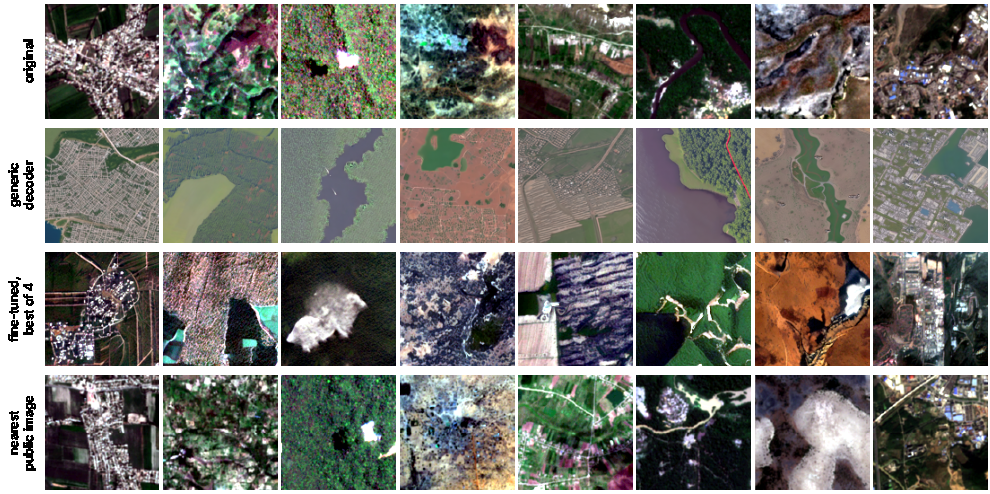
\includegraphics[width=\linewidth]{gen/fig_generic_ft.pdf}
\caption{The first eight attacked VertiBench test images (contrast-stretched for display, as the two bottom rows), the output of the generic decoder of Fig.~\ref{fig:generic}, the best of \giftNBest{} samples of the same decoder fine-tuned on public in-domain pairs, and the public image nearest to the upload in CLIP-L space, which is always of a training location.}\label{fig:generic-ft}
\end{figure}

\begin{figure}[tbp]
\centering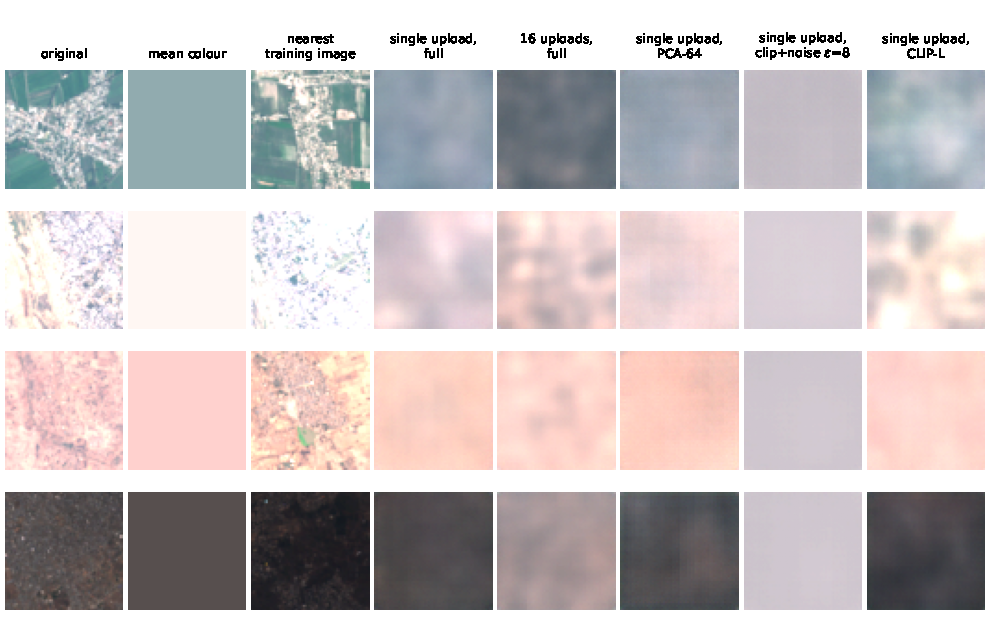
\includegraphics[width=\linewidth]{gen/fig_inversion.pdf}
\caption{Decoders trained on in-domain image--feature pairs, on held-out VertiBench test images ($64\times64$ RGB thumbnails, brightness $\times3$ for display). From left to right: original; its mean colour; nearest training image in DINOv2-g feature space; decoder output from one full DINOv2-g upload, from a PCA-64 upload, from a clipped noisy upload, and from one CLIP-L upload.}\label{fig:inversion}
\end{figure}

\begin{table}[tbp]
\caption{Utility versus leakage of the upload format on VertiBench (DINOv2-g, 224\,px). Accuracy on the test set (5 seeds); PSNR and SSIM of the single-upload inversion; re-identification (top-1, $16\times16$ thumbnails) of the source among the 12{,}560 test images and of its location among the \invNLoc{} test locations. Each value is that of the strongest attacker: the deconvolutional decoder trained for \invEpochs{} epochs, the same trained for \invShortEpochs{} epochs ($^{s}$) or the linear decoder ($^{\ell}$). Clip + noise: per-party Gaussian mechanism, per-upload $(\varepsilon, 10^{-5})$.}\label{tab:privacy}
\centering\scriptsize
\setlength{\tabcolsep}{3.5pt}
\begin{adjustbox}{max width=\linewidth}
\begin{tabular}{@{}lrccccc@{}}
\toprule
 & & & & & \multicolumn{2}{c@{}}{Re-id (\%)}\\\cmidrule(l){6-7}
Upload format & Upload & Acc. (\%) & PSNR (dB) & SSIM & image & location\\
\midrule
\inputtab{gen/tab_privacy.tex}
\bottomrule
\end{tabular}
\end{adjustbox}
\end{table}

\begin{table}[tbp]
\caption{Party-side transforms of the CLIP-L upload on VertiBench. Accuracy of the usual head on the 16 transformed uploads (3 seeds). Linkage: share of the \giVbNTest{} test uploads of a party whose embedding, mapped back to CLIP space from $k$ leaked image--upload pairs of that party ($k=0$: spectral alignment with public in-domain features), is closer to the true CLIP embedding of its image than to that of any other test image (chance \giVbChance\,\%). Raw uploads need no map: the public projection gives the embedding itself.}\label{tab:defences}
\centering\scriptsize
\setlength{\tabcolsep}{4pt}
\begin{tabular}{@{}lrcccccc@{}}
\toprule
& & & \multicolumn{5}{c@{}}{Linkage (\%) with $k$ leaked pairs}\\\cmidrule(l){4-8}
Transform & Dim. & Acc. (\%) & 0 & 10 & 100 & 1{,}000 & 3{,}142\\
\midrule
\inputtab{gen/tab_defences.tex}
\bottomrule
\end{tabular}
\end{table}

\FloatBarrier

\section{Reproducibility}\label{app:repro}

This appendix lists the code, data, compute and training details behind every result of the paper.

\paragraph{Code, data and compute.}
All code, configurations, raw result files and the scripts that generate every table, figure and quoted number from them are in the accompanying repository\footnote{\url{https://github.com/xavierxav/Simple-VFL}, directories \texttt{paper\_experiments} and \texttt{paper\_results}.}. All data sets are public. Each frozen head trains in seconds to minutes on one GPU; the whole study, including the end-to-end baselines, the image augmentation and the WorldStrat feature extraction, used about 110 Google Colab compute units on L4 and A100 GPUs.

\paragraph{Encoders and features.}
All encoders are used through their pooled output token at their native 224\,px input: DINOv2 ViT-S/B/L/g~\cite{oquab2024dinov2}, CLIP ViT-B/16 and ViT-L/14~\cite{radford2021clip}, SigLIP ViT-B/16~\cite{zhai2023siglip}, a supervised ImageNet ResNet-50 and a randomly initialised ViT-B; SSL4EO-S12 ViT-S/16~\cite{wang2023ssl4eo} on all 13 Sentinel-2 bands; BiomedCLIP~\cite{zhang2023biomedclip} and MONET~\cite{kim2024monet} for MILK10k. Satellite images are standardised per band with statistics of the released data (on WorldStrat, estimated on 200 random areas of all folds, without labels) and fed as RGB or as false-colour composites (B8-B4-B3, B12-B8A-B4) to expose the infrared bands to RGB encoders; the SPOT image is encoded at its own pixel count (1050, 518, 266 and 168\,px for 1.5, 3, 6 and 10\,m). Natural images use each model's own normalisation. Features are extracted once in half precision; a party holding several images of an entity (revisits, views) averages their features.

\paragraph{Heads.}
The reference head is a two-layer MLP ($Kd\to1000\to C$, batch normalisation, ReLU; 24.6\,M weights for 16 DINOv2-g parties, 3.1\,M for two). \emph{Late fusion} trains one MLP per party and averages their log-probabilities with a weight $w$ (chosen on the validation fold, or fixed to $\tfrac12$). A \emph{branch} head projects each party to 512 dimensions (linear, LayerNorm, GELU), classifies their concatenation, adds one auxiliary classifier per party (loss weight $\tfrac12$) and, with modality dropout, zeroes one random party in 30\,\% of the training samples. A \emph{pooling} head normalises each party's vector (LayerNorm), averages them over the parties present and applies the MLP; it requires all parties to share an encoder and feature space. A \emph{set} head applies one weight-shared MLP to each of the vectors of a party that holds several images and pools them by attention before the classifier. All heads on frozen features use Adam (learning rate $10^{-3}$, batch 512), at most 50 epochs, \texttt{ReduceLROnPlateau} and early stopping on the unweighted validation loss; the best validation checkpoint is tested (Table~\ref{tab:milkreg} checks two other stopping rules). On the imbalanced WorldStrat and MILK10k labels the loss is class-balanced and macro F1 is the primary metric.

\paragraph{Seeds, folds and tests.}
On VertiBench the public split is used as is (3{,}142 training and 785 test samples); 15\,\% of the training samples are held out for validation with the seed, so seeds change the initialisation and the validation subset, not the test set. We report mean\,$\pm$\,sample standard deviation over five seeds (VertiBench, unless noted), three seeds (CIFAR, ModelNet40; five for the protocol of Sun et al.) or five stratified cross-validation folds (WorldStrat, grouped by site; MILK10k, over lesions), where fold $f$ is the test set and fold $f{+}1$ the validation set. On the fixed VertiBench test set, comparisons use paired bootstrap intervals and exact McNemar tests on test predictions from seed-averaged probabilities (App.~\ref{app:audit}); WorldStrat and MILK10k comparisons are paired by fold. On MILK10k, the age imputation and standardisation of the metadata party are computed on all lesions, without labels.

\paragraph{Baselines.}
\emph{VertiBench recipe}: our re-implementation of the published SplitNN configuration (one ResNet-18 per party with a $9\times9$ stride-2 input convolution, MLP aggregation, Adam with learning rate $10^{-5}$, step decay, batch 32, 50 epochs, last epoch tested, 16 bottoms run sequentially) on the 13 bands. \emph{SplitNN, our recipe}: standard ResNet-18 bottoms~\cite{he2016resnet}, from scratch or ImageNet weights, and the same MLP top model as our head (Adam, one-cycle schedule, 40 epochs, batch 64, flips, best validation checkpoint). \emph{FedOnce}~\cite{wu2022fedonce}: every party trains a ResNet-18 on its unlabelled training images with Noise As Targets~\cite{bojanowski2017nat} (64-d targets, Hungarian re-assignment every 3 epochs, 100 epochs) or SimCLR~\cite{chen2020simclr} and uploads its output once; each party's encoder is pre-trained once and the five seeds re-train the head only, so the standard deviation of these rows is conditional on that pre-training. \emph{Same-backbone split learning}: frozen and LoRA-adapted CLIP ViT-B/16 bottoms on VertiBench; frozen, LoRA-adapted and (for DINOv2) fully fine-tuned CLIP ViT-B/16 and DINOv2 ViT-B/14 bottoms on MILK10k, with ResNet-18 baselines from scratch and from ImageNet weights. LoRA~\cite{hu2022lora} uses rank 16 on the attention query and value projections; the ViT runs use 10 epochs, augmentation and the best validation checkpoint, with a class-balanced loss on MILK10k. These baselines follow published or standard recipes without extensive hyper-parameter search.
.
% Every number is a macro of gen/macros.tex or a value quoted from the published papers.

\section{Full VertiBench results and encoders}\label{app:vb}

This appendix supports both contributions: it details the VertiBench baselines and the comparison of frozen encoders behind the foundation-model points of the frontier (C1), and shows how accuracy depends on the number of parties of this benchmark (C2).

\begin{table}[tbp]
\caption{VertiBench Satellite, all methods (16 parties, official test set). Upload: training payload per sample over all parties (activations or logits up, gradients down when needed). GFLOPs: party compute per image (a training run for split learning, one forward pass otherwise). Time: minutes on one A100 (split training, FedOnce pre-training or feature extraction). Mean\,$\pm$\,std over 5 seeds unless noted; --: not recorded.}\label{tab:main}
\centering\scriptsize
\setlength{\tabcolsep}{3pt}
\begin{adjustbox}{max width=\linewidth}
\begin{tabular}{@{}lcrrrccc@{}}
\toprule
Method & Bands & Upload & GFLOPs & Time & Acc. (\%) & F1 (\%) & AUC (\%)\\
\midrule
\inputtab{gen/tab_main.tex}
\bottomrule
\end{tabular}
\end{adjustbox}
\end{table}

\paragraph{Baselines.}
Our re-implementation of the published VertiBench split-learning configuration reaches $\reproAcc\pm\reproStd$\,\% on the 13 bands after its last epoch, in line with the published $81.2\pm0.4$\,\% (Table~\ref{tab:main}). Our own split-learning recipe is weaker from scratch (\splitAllAcc\,\% on 13 bands, \splitRGBAcc\,\% on RGB) and matches it from ImageNet weights (\splitPTAcc\,\% on RGB). FedOnce, whose parties learn their encoder on their own unlabelled images before a single upload, reaches \natAcc\,\% with Noise As Targets and \sslAllAcc\,\% with SimCLR: on 3{,}142 training locations, self-supervised training does not produce better features than supervised split learning. Macro F1 and AUC order the frozen foundation encoders above these baselines as accuracy does, but not among themselves (CLIP-B has the best macro F1 and a lower accuracy than CLIP-L). No difference between the two best encoders is detected: on the same test predictions (seed-averaged probabilities), CLIP-L leads DINOv2-g by $\pairDiff$ points, 95\,\% bootstrap interval $[\pairLo, \pairHi]$, McNemar $p=\pairP$.

\paragraph{Encoder choice.}
Table~\ref{tab:encoders} compares nine frozen encoders under the same head. All pre-trained ViTs lie between 81.6 and 85.2\,\%, a supervised ImageNet ResNet-50 reaches 80.9\,\%, and a randomly initialised ViT-B only 75.1\,\%: the gain comes from pre-training, not from the head. Size matters moderately: DINOv2 gains 2.4 points from ViT-S/14 (81.8\,\%) to ViT-g/14 (84.2\,\%), whereas CLIP ViT-B/16 is within one point of ViT-L/14. In FLOPs a large encoder is not cheaper than training a small bottom model: one DINOv2-g pass costs \vbGGF{} GFLOPs per image, more than the \rEighteenTrainGF{} GFLOPs of 50 training epochs of the VertiBench ResNet-18 bottom, whereas CLIP-B costs \vbClipBGF{} GFLOPs; encoding all images of the 16 parties takes \vbGMin{} minutes with DINOv2-g and \vbClipBMin{} with CLIP-B on one A100. Parties may also upload the features of two encoders side by side: CLIP-L with CLIP-B reaches \comboLB\,\%, DINOv2-g with CLIP-L \comboGL\,\%, a small gain for a larger upload. The encoder is therefore a parameter of the regime, chosen for cost.

\paragraph{Number of parties.}
The 16 VertiBench parties observe the same sensor at different dates and are largely redundant: with DINOv2-g, one party alone gives \soloMean\,\% on average (\soloMin--\soloMax), two parties \partiesKTwo\,\%, four \partiesKFour\,\%, eight \partiesKEight\,\% and all 16 \partiesKAll\,\% (Fig.~\ref{fig:parties}, left). This redundancy is a property of the benchmark: it limits what any method can gain by combining parties here, and it lets a suitable head tolerate missing parties (App.~\ref{app:pca}).

\begin{table}[tbp]
\caption{Frozen encoders on VertiBench (224\,px RGB, one upload, 5 seeds). Params in millions, GFLOPs per image, $d$ per party. Bottom: each party uploads two encoders' features side by side (features standardised).}\label{tab:encoders}
\centering\scriptsize
\setlength{\tabcolsep}{3.5pt}
\begin{adjustbox}{max width=\linewidth}
\begin{tabular}{@{}lrrrccc@{}}
\toprule
Encoder & Params & GFLOPs & $d$ & Acc. (\%) & F1 (\%) & Linear acc. (\%)\\
\midrule
\inputtab{gen/tab_encoders.tex}
\midrule
\multicolumn{7}{@{}l}{\emph{Each party uploads two encoders' features (standardised)}}\\
\inputtab{gen/tab_combo_enc.tex}
\bottomrule
\end{tabular}
\end{adjustbox}
\end{table}

\begin{figure}[tbp]
\centering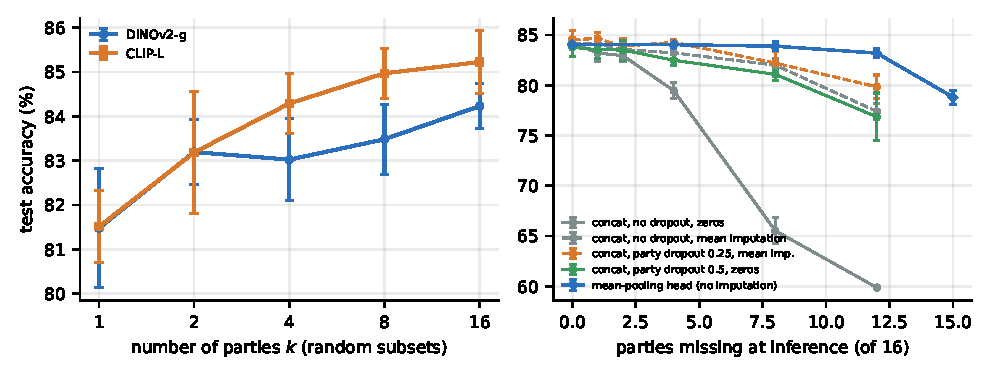
\includegraphics[width=\linewidth]{gen/fig_parties.pdf}
\caption{VertiBench, DINOv2-g. Left: accuracy with $k$ randomly chosen parties (3 subsets $\times$ 5 seeds). Right: parties missing at inference for a concatenation head (missing uploads replaced by zeros or by the party's training mean, with and without party dropout during training) and for a head that averages per-party embeddings.}\label{fig:parties}
\end{figure}

\FloatBarrier

\section{Compression grid}\label{app:pca}

This appendix supports contribution C1: it gives the full grid of local PCA and quantisation from which the main text takes the knee of the frontier, and the limits of compressing without coordination.

\paragraph{Protocol.}
Because the encoder is frozen, each party can fit a PCA on its own training features (keeping $d'\le d$ components; the basis stays with the party) and quantise every coordinate uniformly to $b$ bits between its 1st and 99th training percentiles. The label owner trains the head on the de-quantised values. No labels, shared basis or coordination are needed, but the samples must still be aligned across parties; the few hundred bytes of quantiser bounds that each party sends once are not counted.

\paragraph{Selection under a byte budget.}
On frozen DINOv2-g features we run the grid of Table~\ref{tab:pareto} (16 to 512 components or no PCA, 1 to 16 bits) and select, under each budget, the configuration with the best \emph{validation} accuracy (Fig.~\ref{fig:pareto}). For the 16 parties together, 256\,B per sample (\selTwoCfg) give \selTwoAcc\,\%, 512\,B (\selFiveCfg) \selFiveAcc\,\%, 2\,KiB (\selTwokCfg) \selTwokAcc\,\%, and the full budget selects \selFullCfg{} (\selFullBytes) at \selFullAcc\,\%, against \fullAcc\,\% for the uncompressed 48\,KiB. Moderate compression therefore costs nothing on this benchmark; with 4 bits or more, the PCA-256 and PCA-512 rows are even slightly above the uncompressed features, which we attribute, without having tested it, to a regularising effect on the small labelled set. Even one bit per feature keeps \cmpOneBit\,\%.

\paragraph{Other benchmarks.}
Compression is not free everywhere. On MILK10k a per-party PCA-256 slightly lowers the macro F1 of the concatenation head (\mrGPca, \mrCPca{} and \mrMPca\,\% against \mrGCat, \mrCCat{} and \mrMCat\,\% with DINOv2-g, CLIP-L and MONET; Table~\ref{tab:milkreg}). On WorldStrat, PCA-256 per party changes IPCC and LCCS F1 by \wpIpccPca{} and \wpLccsPca{} points relative to concatenation of the same inputs (Table~\ref{tab:wsfusion}).

\paragraph{Missing parties.}
A concatenation head breaks when parties are missing at inference and their uploads are replaced by zeros (\missZeroEightZ\,\% with 8 of 16 missing, \missZeroTwelveZ\,\% with 12); imputing the party's training mean (\missZeroTwelveM\,\% with 12 missing) or training with party dropout 0.5 (\missHTwelveZ\,\%) repairs most of it (Fig.~\ref{fig:parties}, right). A pooling head (App.~\ref{app:repro}) needs neither: it reaches \poolGMean\,\% with all parties, \poolMissTwelve\,\% with 12 missing and still \poolMissFifteen\,\% with a single party left. It requires a shared feature space, however, and uncoordinated compression removes it: after per-party PCA-64, whose bases differ between parties, the pooling head drops to \poolGPcaMean\,\%, while concatenation of the same uploads keeps \poolGPcaConcat\,\%. Nor does it apply to parties with different modalities or encoders. Local compression and robustness to missing parties must thus be traded off, unless the parties agree on a common basis (e.g.\ one fitted on public images; not tested).

\begin{figure}[tbp]
\centering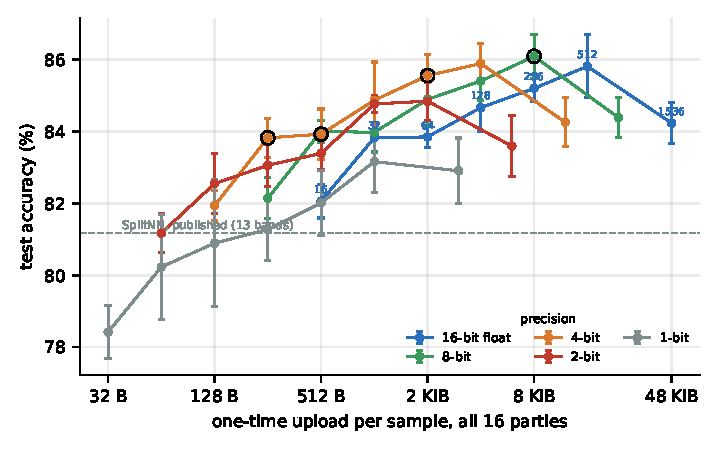
\includegraphics[width=0.78\linewidth]{gen/fig_pareto.pdf}
\caption{VertiBench: accuracy versus one-time upload (bytes per sample, 16 parties) for per-party PCA (number of components annotated on the 16-bit curve) and uniform scalar quantisation of frozen DINOv2-g features, MLP head, 5 seeds. Circles: configuration with the best \emph{validation} accuracy under a budget of 256\,B, 512\,B, 2\,KiB and 48\,KiB.}\label{fig:pareto}
\end{figure}

\begin{table}[tbp]
\caption{The compression grid of Fig.~\ref{fig:pareto} (VertiBench, DINOv2-g, MLP head, 5 seeds). $d'$: PCA components per party (1536: no PCA); $b$: bits per coordinate; upload: one-time payload per sample over the 16 parties. Validation accuracy (seed mean) is the selection criterion; test accuracy and AUC are mean\,$\pm$\,std.}\label{tab:pareto}
\centering\scriptsize
\setlength{\tabcolsep}{4pt}
\begin{tabular}{@{}rrrccc@{}}
\toprule
$d'$ & $b$ & Upload & Val.\ acc.\ (\%) & Test acc.\ (\%) & AUC (\%)\\
\midrule
\inputtab{gen/tab_pareto.tex}
\bottomrule
\end{tabular}
\end{table}

\FloatBarrier

\section{VertiBench audit}\label{app:audit}

This appendix supports contribution C2: it details the audit of the official VertiBench Satellite split and the paired tests behind the comparisons with SplitNN in the main text.

\paragraph{Mapping to source areas.}
Image fingerprints match \auMapTrain{} training and \auMapTest{} test samples to distinct WorldStrat areas (5th-percentile correlation \auScore); \auMapOverlap{} areas appear in both splits.

\paragraph{Siblings, confounded with class.}
The split is not grouped by site, however: \auSibN{} test samples (\auSibShare\,\%) have a training tile from the same site, all from the two sources whose sites are cut into $3\times3$ tiles. They account for \auSibN{} of the 113 test samples in classes 0 and 1, so the \auNoSibN{} test samples without a known sibling are almost all of classes 2 and 3, and class and sibling effects cannot be separated. Table~\ref{tab:audit} gives each head's accuracy on the two subsets. SplitNN is markedly more accurate with siblings (\auSnSib{} vs.\ \auSnNoSib\,\%); the one-shot heads are similarly accurate on both (CLIP-L: \auClipSib{} vs.\ \auClipNoSib\,\%), and the four-logit CLIP heads and frozen split learning are \emph{less} accurate with siblings. The margins over SplitNN are therefore larger on the subset without siblings.

\paragraph{Paired tests.}
The three-seed SplitNN re-run that retains test probabilities averages \auSnAll\,\% accuracy, versus \reproAcc\,\% over five seeds in Table~\ref{tab:main}. We pair test predictions after averaging probabilities over the same three seeds per method (exact McNemar test and 95\,\% paired bootstrap interval, 10{,}000 resamples). On the whole test set, the two CLIP one-shot MLPs, the three four-logit heads and CLIP-B split learning with LoRA beat SplitNN at the 5\,\% level; DINOv2-g's one-shot MLP ($+\pairSnGDiff$ points, $p\pairSnGP$) and frozen CLIP-B split learning do not (Table~\ref{tab:audit}). In detail, the CLIP-L, CLIP-B and DINOv2-g one-shot heads gain $\pairSnClipDiff$ ($p\pairSnClipP$), $\pairSnClipBDiff$ ($p\pairSnClipBP$) and $\pairSnGDiff$ points ($p\pairSnGP$); the CLIP-L, DINOv2-g and CLIP-B four-logit heads give $p\pairSnLgClipP$, $p\pairSnLgGP$ and $p\pairSnLgClipBP$, LoRA split learning $p\pairSnLoraP$ and frozen split learning $p\pairSnSplitFrozenP$. Without known siblings every margin grows and all are significant (CLIP-L: $\pairSnClipNoSibDiff$ points, $p\pairSnClipNoSibP$). These $p$-values are uncorrected: after a Holm correction over the \holmN{} comparisons, \holmSurvive{} remain below 0.05, LoRA split learning and the CLIP-B four-logit head. LoRA itself is unstable across seeds (\seedLoraMin{} to \seedLoraMax\,\%); paired with the ensemble of the one-shot CLIP-B head on the same seeds, its lead is $\pairLoraHeadDiff$ points ($[\pairLoraHeadLo,\pairLoraHeadHi]$, $p\pairLoraHeadP$).

\paragraph{Nearest public image.}
The retrieval attacker of App.~\ref{app:privacy} does not owe its success to siblings: across test uploads, the label of the nearest public training image in CLIP-L space matches in \nnPubAll\,\% of the cases (\nnPubSib\,\% with known siblings, \nnPubNoSib\,\% without), and the neighbour is itself a sibling in just \nnPubIsSib\,\% of the sibling cases, about 5\,\% overall.

\begin{table}[tbp]
\caption{VertiBench audit. Test accuracy (\%) on all 785 test samples, on the \auSibN{} with a training tile from the same site and on the \auNoSibN{} without; paired gain over SplitNN in points with 95\,\% paired bootstrap interval and exact McNemar test, on all samples and without siblings. Probabilities averaged over 3 seeds per method.}\label{tab:audit}
\centering\scriptsize
\setlength{\tabcolsep}{3pt}
\begin{adjustbox}{max width=\linewidth}
\begin{tabular}{@{}lccccccc@{}}
\toprule
& \multicolumn{3}{c}{Accuracy (\%)} & \multicolumn{2}{c}{Gain over SplitNN, all} & \multicolumn{2}{c@{}}{Gain, no sibling}\\
\cmidrule(lr){2-4}\cmidrule(lr){5-6}\cmidrule(l){7-8}
Head & all & sibling & no sibling & points [95\,\% CI] & McNemar & points [95\,\% CI] & McNemar\\
\midrule
SplitNN, VertiBench recipe & \auSnAll & \auSnSib & \auSnNoSib & -- & -- & -- & --\\
\midrule
One-shot MLP, CLIP-L & \auClipAll & \auClipSib & \auClipNoSib & $\pairSnClipDiff$ $[\pairSnClipLo,\pairSnClipHi]$ & $p\pairSnClipP$ & $\pairSnClipNoSibDiff$ $[\pairSnClipNoSibLo,\pairSnClipNoSibHi]$ & $p\pairSnClipNoSibP$\\
One-shot MLP, CLIP-B & \auClipBAll & \auClipBSib & \auClipBNoSib & $\pairSnClipBDiff$ $[\pairSnClipBLo,\pairSnClipBHi]$ & $p\pairSnClipBP$ & $\pairSnClipBNoSibDiff$ $[\pairSnClipBNoSibLo,\pairSnClipBNoSibHi]$ & $p\pairSnClipBNoSibP$\\
One-shot MLP, DINOv2-g & \auGAll & \auGSib & \auGNoSib & $\pairSnGDiff$ $[\pairSnGLo,\pairSnGHi]$ & $p\pairSnGP$ & $\pairSnGNoSibDiff$ $[\pairSnGNoSibLo,\pairSnGNoSibHi]$ & $p\pairSnGNoSibP$\\
\midrule
Four-logit head, CLIP-L & \auLgClipAll & \auLgClipSib & \auLgClipNoSib & $\pairSnLgClipDiff$ $[\pairSnLgClipLo,\pairSnLgClipHi]$ & $p\pairSnLgClipP$ & $\pairSnLgClipNoSibDiff$ $[\pairSnLgClipNoSibLo,\pairSnLgClipNoSibHi]$ & $p\pairSnLgClipNoSibP$\\
Four-logit head, CLIP-B & \auLgClipBAll & \auLgClipBSib & \auLgClipBNoSib & $\pairSnLgClipBDiff$ $[\pairSnLgClipBLo,\pairSnLgClipBHi]$ & $p\pairSnLgClipBP$ & $\pairSnLgClipBNoSibDiff$ $[\pairSnLgClipBNoSibLo,\pairSnLgClipBNoSibHi]$ & $p\pairSnLgClipBNoSibP$\\
Four-logit head, DINOv2-g & \auLgGAll & \auLgGSib & \auLgGNoSib & $\pairSnLgGDiff$ $[\pairSnLgGLo,\pairSnLgGHi]$ & $p\pairSnLgGP$ & $\pairSnLgGNoSibDiff$ $[\pairSnLgGNoSibLo,\pairSnLgGNoSibHi]$ & $p\pairSnLgGNoSibP$\\
\midrule
Split learning, CLIP-B frozen & \auSplitFrozenAll & \auSplitFrozenSib & \auSplitFrozenNoSib & $\pairSnSplitFrozenDiff$ $[\pairSnSplitFrozenLo,\pairSnSplitFrozenHi]$ & $p\pairSnSplitFrozenP$ & $\pairSnSplitFrozenNoSibDiff$ $[\pairSnSplitFrozenNoSibLo,\pairSnSplitFrozenNoSibHi]$ & $p\pairSnSplitFrozenNoSibP$\\
Split learning, CLIP-B LoRA & \auLoraAll & \auLoraSib & \auLoraNoSib & $\pairSnLoraDiff$ $[\pairSnLoraLo,\pairSnLoraHi]$ & $p\pairSnLoraP$ & $\pairSnLoraNoSibDiff$ $[\pairSnLoraNoSibLo,\pairSnLoraNoSibHi]$ & $p\pairSnLoraNoSibP$\\
\bottomrule
\end{tabular}
\end{adjustbox}
\end{table}

\FloatBarrier

\section{MILK10k details}\label{app:milk}

This appendix supports contribution C1: it gives the party combinations, fusion heads and regularisation checks behind the frozen MILK10k rows of Table~\ref{tab:freeze}, and the same-recipe comparison of frozen and adapted backbones. Figure~\ref{fig:frontier-axes-milk} places the MILK10k points on the other axes of the cost accounting: one-shot points need \frMilkRoundsMatch{} message against \frMilkRoundsSplitNN{} for ResNet-18 split learning, and \frMilkGflopsMatchName{} exceeds that baseline (\frMilkGflopsMatchAcc{} vs.\ \frMilkBestNonFound\,\%) with \frMilkGflopsRatio{} times less party compute.

\begin{figure}[t]
\centering\IfFileExists{gen/fig_frontier_axes_milk.pdf}{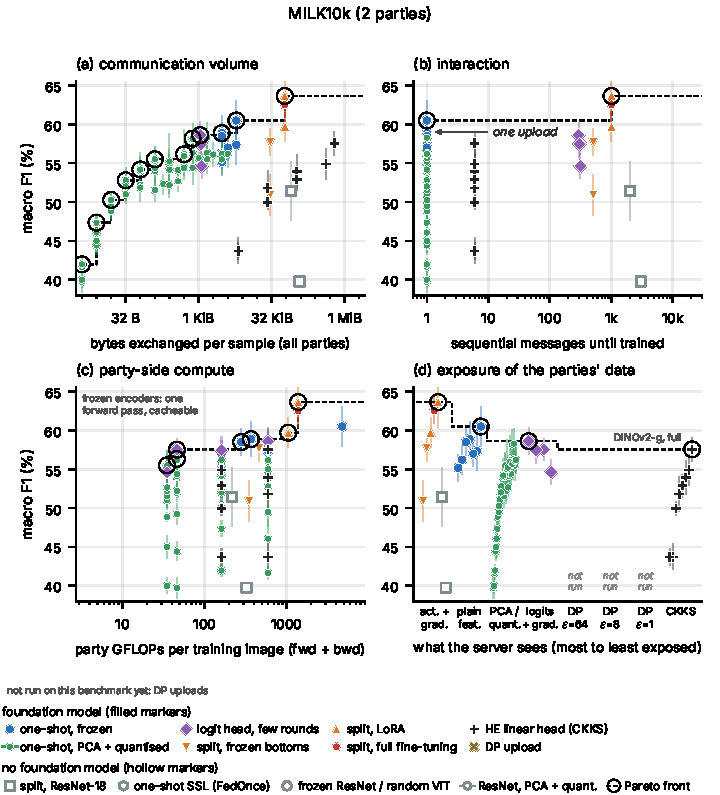
\includegraphics[width=\linewidth]{gen/fig_frontier_axes_milk.pdf}}{\fbox{\parbox{0.9\linewidth}{\centering fig\_frontier\_axes\_milk pending}}}
\caption{MILK10k along the axes of Fig.~\ref{fig:frontier-axes}: (a)~bytes per training sample, (b)~sequential messages until trained, (c)~party GFLOPs per training image (forward and backward), (d)~exposure ladder. Only DP is marked as not run. Circled: Pareto-optimal points.}\label{fig:frontier-axes-milk}
\end{figure}

\begin{table}[tbp]
\caption{MILK10k, all methods (2 parties, 5 folds, class-balanced loss). Split learning trains the bottoms with the server's gradients; one-shot rows use frozen features and an MLP head (concatenation, or late fusion on features averaged over 8 rotations and flips). Upload per training sample: over all training epochs for split learning (30 for ResNet-18 from scratch, 20 from ImageNet, 10 for ViTs), once for one-shot. Time: minutes per fold (one-shot: encoding, estimated).}\label{tab:freeze}
\centering\scriptsize
\setlength{\tabcolsep}{3pt}
\begin{adjustbox}{max width=\linewidth}
\begin{tabular}{@{}llrrrccc@{}}
\toprule
Party models & Training & Trainable & Upload & Time & F1 (\%) & Bal.\ acc.\ (\%) & Acc.\ (\%)\\
\midrule
\inputtab{gen/tab_freeze.tex}
\bottomrule
\end{tabular}
\end{adjustbox}
\end{table}

\paragraph{Real modalities complement each other little.}
The dermoscopic image alone gives \milkGDerm\,\% macro F1 with DINOv2-g, the clinical photograph \milkGClin\,\%, the metadata \milkMeta\,\% (Table~\ref{tab:milk}). Concatenating the two images adds less than one point over the dermoscopy (\milkGBoth\,\%), three points with CLIP-L (\milkCDerm{} $\to$ \milkCBoth\,\%); the metadata add at most one point on top. The general-purpose encoders match or beat the medical ones (BiomedCLIP, MONET). Splitting the dermoscopy into two halves, as split benchmarks do, \emph{loses} information instead: \milkGHalves\,\% against \milkGDerm\,\% for the whole image, because each party's encoder sees half a lesion. Two caveats apply to all MILK10k numbers: folds are drawn over lesions, as the release has no patient identifiers, and each test fold holds only 40 to 61 lesions of the two rarest classes.

\paragraph{How the parties are combined matters as much as the encoder.}
A concatenation MLP under-uses the weaker party. Training one head per party and averaging their log-probabilities (late fusion) is better for every encoder (Table~\ref{tab:milkfusion}): \mfGLate\,\% instead of \mfGCat\,\% with DINOv2-g, \mfCLate\,\% instead of \mfCCat\,\% with CLIP-L, \mfGMLate\,\% when each party uploads DINOv2-g and MONET features; with DINOv2-g, the two parties together then reach \mfGLate\,\%, about three points more than the dermoscopic party alone (\milkGDerm\,\%). Late fusion also suits VFL: each party's head can be trained, audited and dropped independently. The gain is bounded by the data: \mfGBoth\,\% of the lesions are misclassified by both single-party heads, against \mfGIndep\,\% if their errors were independent---the two modalities fail on the same, intrinsically hard lesions.

\paragraph{Over-fitting or modality competition?}
With 3{,}100 training lesions and 2--3k input dimensions, the concatenation head could simply over-fit. Three observations speak against this being the main cause (Table~\ref{tab:milkreg}). First, regularising it---input dropout, Gaussian feature noise, feature mixup, a per-party PCA---gains at most one point and never reaches late fusion. Second, late fusion does not need its tuned weight: a fixed weight of 0.5 does as well (\mrGLateHalf\,\% with DINOv2-g); paired by fold, it beats concatenation by \mrGPairD\,$\pm$\,\mrGPairS{} points with DINOv2-g (\mrGPairW{} folds out of 5), \mrCPairD\,$\pm$\,\mrCPairS{} with CLIP-L (\mrCPairW/5) and \mrMPairD\,$\pm$\,\mrMPairS{} with MONET (\mrMPairW/5). Third, its advantage does not shrink with more data, as over-fitting would predict: it grows from 25\,\% to 100\,\% of the training folds for CLIP-L and MONET. Nor is it an artefact of our early-stopping rule on the unweighted validation loss: when both heads stop on the class-weighted validation loss or on the validation macro F1, late fusion still wins by \mrStopMin{} to \mrStopMax{} points over \mrStopN{} comparisons (DINOv2-g, CLIP-L, DINOv2-B, CLIP-B; stopping on the weighted loss lowers every head by up to \mrWlossDropMax{} points), and weight decay on the concatenation head leaves a gap of \mrWdMin{} to \mrWdMax{} points. The pattern rather matches the \emph{modality competition} documented for jointly trained multimodal networks~\cite{wang2020makes,huang2022modality,peng2022balanced}: a joint head learns the dominant dermoscopy first and stops before exploiting the clinical photograph, whereas separate heads must each use their own modality fully; the validation-tuned late fusion gives the weaker clinical party a weight of 0.3 to 0.5. Augmentation helps in image space, not in feature space: the parties can encode the 8 rotations and flips of each photograph once (8 times the encoding cost) and upload the mean, which raises late fusion to \mrGLateViews\,\% (DINOv2-g), \mrMLateViews\,\% (MONET), \fzViewsB\,\% (DINOv2-B) and \fzViewsCb\,\% (CLIP-B) at no extra communication. With CLIP-L it helps late fusion little (\mrCLateViews\,\%); there the best head is the concatenation trained on one of the 8 uploaded views per epoch (\mrCCatSampled\,\%, at 8 times the upload).

\paragraph{Frozen versus adapted under the same recipe.}
The frozen and adapted rows of Table~\ref{tab:freeze} differ in more than freezing (augmentation, head, standardisation, optimiser and schedule). In a paired re-run we therefore use the same split-learning recipe with frozen and LoRA bottoms. For DINOv2-B this gives \srFrozenB\,\% macro F1 frozen versus \srLoraB\,\% with LoRA (paired gain $\srGapB\pm\srGapSdB$ points, \srWinsB/5 folds); for CLIP-B, \srFrozenCb\,\% versus \srLoraCb\,\% ($\srGapCb\pm\srGapSdCb$ points, \srWinsCb/5 folds). Relative to the one-shot MLPs, freezing under the split recipe shifts F1 by $\srVsHeadB$ and $\srVsHeadCb$ points, respectively, so the larger same-recipe LoRA gain for CLIP-B partly reflects its weaker frozen baseline under that recipe. Adaptation wins on MILK10k under both recipes.

\begin{table}[tbp]
\caption{MILK10k: macro F1 (\%) of one-shot heads on frozen features for every combination of parties (5 folds, class-balanced MLP head). Bottom: the usual practice of splitting one image into a left and a right party.}\label{tab:milk}
\centering\scriptsize
\setlength{\tabcolsep}{3.5pt}
\begin{adjustbox}{max width=\linewidth}
\begin{tabular}{@{}lcccc@{}}
\toprule
Parties & \inputtab{gen/tab_milk_head.tex}\\
\midrule
\inputtab{gen/tab_milk.tex}
\bottomrule
\end{tabular}
\end{adjustbox}
\end{table}

\begin{table}[tbp]
\caption{MILK10k: how the label owner combines the clinical (A) and dermoscopic (B) uploads (macro F1, \%, 5 folds). Late fusion: one head per party, log-probabilities averaged with a weight chosen on the validation fold. Branches: per-party projection, auxiliary per-party losses and modality dropout (0.3). Last column: share of test lesions misclassified by both single-party heads, and (in brackets) what it would be if their errors were independent.}\label{tab:milkfusion}
\centering\scriptsize
\setlength{\tabcolsep}{3pt}
\begin{adjustbox}{max width=\linewidth}
\begin{tabular}{@{}lcccccc@{}}
\toprule
Encoder & B alone & A+B concat & A+B late fusion & A+B branches & A+B+C branches & Both wrong (\%)\\
\midrule
\inputtab{gen/tab_milkfusion.tex}
\bottomrule
\end{tabular}
\end{adjustbox}
\end{table}

\begin{table}[tbp]
\caption{MILK10k, clinical + dermoscopic parties: is the concatenation head over-fitting? Macro F1 (\%, 5 folds). Top: regularising the concatenation head versus late fusion. Middle: augmentation precomputed once by the parties (8 rotations and flips of each photograph). Bottom: gap between late fusion (fixed weight) and concatenation when the training folds are subsampled, and under other early-stopping rules than the unweighted validation loss.}\label{tab:milkreg}
\centering\scriptsize
\setlength{\tabcolsep}{3.5pt}
\begin{adjustbox}{max width=\linewidth}
\begin{tabular}{@{}lccc@{}}
\toprule
Head & DINOv2-g & CLIP-L & MONET\\
\midrule
\inputtab{gen/tab_milkreg.tex}
\bottomrule
\end{tabular}
\end{adjustbox}
\end{table}

\FloatBarrier

\section{WorldStrat: two sensors}\label{app:ws}

This appendix supports contribution C2: it reports a third natural partition, with genuinely different sensors, on which the two parties complement each other little once the folds are grouped by site.

\paragraph{Task.}
From the WorldStrat release~\cite{cornebise2022worldstrat} we build a two-party task on its \wsIpccN{} usable areas of $1.58\times1.58$\,km: party A holds the SPOT 6/7 pan-sharpened image (RGB, 1.5\,m, $1050\times1050$ pixels), party B the 16 Sentinel-2 L1C revisits (13 bands, 10\,m). The label owner holds one of three labels of the release metadata, all read at the centre of the area: the LCCS land-cover class of the 300\,m pixel of a global land-cover map~\cite{esa2017cci} (the 18 classes with at least 40 areas), its coarser IPCC category (7 classes), and the degree of urbanisation of the 1\,km SMOD cell (8 classes, from rural very-low-density to urban centre~\cite{pesaresi2019ghsl}). A label therefore describes only the centre of the image (4\,\% of its area for LCCS and IPCC); the parties also encode centre crops of 336\,m and 1\,km. To vary the information held by A, its image is degraded to 3, 6 and 10\,m before encoding, or cut into 16 full-resolution tiles of 262\,px whose features are averaged. Party B encodes every revisit as three composites (RGB, near- and short-wave infrared) and uploads, per composite, the mean over the 16 revisits or over the 8 least cloudy ones (ranked by a locally computed cloud score), possibly with the temporal standard deviation; for a set head it uploads all 16 vectors. The loss is class-balanced and macro F1 is the metric.

\paragraph{Grouped cross-validation.}
The five folds are stratified and grouped by site: all nine tiles of a site stay in the same fold. Stratification alone split sibling tiles across training and test and gave macro F1 about 6 to 9 points higher on the two land-cover tasks---the same leakage as in the official VertiBench split, which is built from the same areas (App.~\ref{app:audit}). All results below are site-grouped and paired by fold.

\paragraph{The second sensor adds little.}
Alone, the 1.5\,m SPOT image scores \wsIpccSpot{} against \wsIpccSms\,\% macro F1 for the Sentinel-2 revisits (RGB, NIR, SWIR) on IPCC, \wsLccsSpot{} against \wsLccsSms\,\% on LCCS and \wsSmodSpot{} against \wsSmodSms\,\% on SMOD (Table~\ref{tab:ws}). Their concatenation reaches \wsIpccFus, \wsLccsFus{} and \wsSmodFus\,\%: relative to SPOT, F1 changes by \wgIpccA{} points on IPCC (\wgIpccAW{} folds improve), \wgLccsA{} on LCCS (\wgLccsAW) and \wgSmodA{} on SMOD (\wgSmodAW). With DINOv2-g, the pair is thus at most a couple of points above the better single sensor on land cover, and below SPOT alone on urbanisation. The second sensor matters more when the first is weakened (Fig.~\ref{fig:ws}): at 3\,m, fusion adds \wgIpccThree{} points on IPCC (\wgIpccThreeW) and \wgLccsThree{} on LCCS (\wgLccsThreeW); at 10\,m, \wgIpccTen{} (\wgIpccTenW) and \wgLccsTen{} (\wgLccsTenW), whereas SMOD never gains (\wgSmodTen{} at 10\,m, \wgSmodTenW). For land cover, SPOT improves alone at 3\,m (\wsIpccSpotThree{} and \wsLccsSpotThree\,\%) or by averaging the features of 16 full-resolution tiles (\wfIpccSpotTiles{} and \wfLccsSpotTiles\,\%), rather than feeding DINOv2 the whole 1{,}050\,px image; adding the clearest revisits to the tiles yields \wpIpccTilesFus{} and \wpLccsTilesFus{} points (\wpIpccTilesFusW{} and \wpLccsTilesFusW). Adding infrared to RGB helps LCCS at native resolution and both land-cover labels at 10\,m. With a multispectral encoder (SSL4EO-S12 on the 13 bands) for party B, or CLIP-L for both parties, fused IPCC scores and their gain over the single sensors are larger (Table~\ref{tab:ws}), while SMOD barely changes; we did not test these rows in pairs. For native-resolution fusion, pooled out-of-fold per-class F1 gains over SPOT are largest for \wcIpccTop{} on IPCC and \wcLccsTop{} on LCCS (points and number of areas); F1 falls in \wcIpccNeg{} IPCC and \wcLccsNeg{} LCCS classes.

\paragraph{Why a second sensor adds little.}
The parties fail on the same areas: on IPCC both are wrong on \wfIpccBoth\,\% of them, nearly three times the \wfIpccIndep\,\% expected from independent errors, although an oracle choosing the right party would reach \wfIpccOracle\,\% accuracy. Context matters more than a second view of the labelled pixel: although labels are read at the centre of the area, the whole 1.58\,km SPOT image beats a 336\,m centre crop by \wpIpccCentre, \wpLccsCentre{} and \wpSmodCentre{} points (\wpIpccCentreW, \wpLccsCentreW{} and \wpSmodCentreW{} folds); with a 1\,km crop, land-cover scores are roughly unchanged and only SMOD still loses ground (\wfSmodSpotCk{} vs.\ \wfSmodSpot\,\%).

\paragraph{Fusion heads do not change the picture.}
No fusion variant of Table~\ref{tab:wsfusion} improves on plain-mean concatenation across all three labels. The set head over the 16 revisits changes F1 by \wpLccsSetCat{} to \wpIpccSetCat{} points while multiplying the Sentinel-2 payload by 16. Late fusion changes IPCC, LCCS and SMOD F1 by \wpIpccLateMean, \wpLccsLateMean{} and \wpSmodLateMean{} points with the plain mean (SMOD improves in \wpSmodLateMeanW{} folds), and by \wpIpccLateCat, \wpLccsLateCat{} and \wpSmodLateCat{} with the clearest-revisit summary, where the branch head trails concatenation by \wpIpccBranch, \wpLccsBranch{} and \wpSmodBranch{} points. Adding temporal standard deviations shifts the IPCC F1 of Sentinel-2 alone by \wpIpccStdSolo{} points (\wpIpccStdSoloW{} folds improve), and adding a centre crop to SPOT alone changes IPCC and LCCS by \wpIpccFC{} and \wpLccsFC{} points.

\begin{table}[tbp]
\caption{WorldStrat, 5 site-grouped folds: macro F1 (\%, mean\,$\pm$\,std) of each sensor alone and of their concatenation (MLP head; DINOv2-g unless noted). A: SPOT image; B: mean of the 16 Sentinel-2 revisits, encoded as RGB, as three composites (RGB, NIR, SWIR) or on all 13 bands by SSL4EO-S12. Note the column order.}\label{tab:ws}
\centering\scriptsize
\setlength{\tabcolsep}{4pt}
\begin{tabular}{@{}lccc@{}}
\toprule
Parties & IPCC & SMOD & LCCS\\
\midrule
\inputtab{gen/tab_ws.tex}
\bottomrule
\end{tabular}
\end{table}

\begin{figure}[tbp]
\centering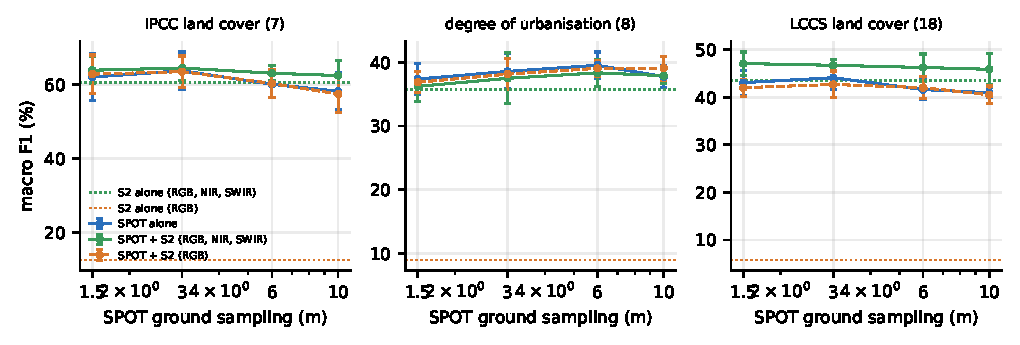
\includegraphics[width=\linewidth]{gen/fig_ws.pdf}
\caption{WorldStrat: macro F1 (mean over 5 site-grouped folds, DINOv2-g, MLP head) of the SPOT party alone and with the Sentinel-2 party, as the SPOT image is degraded from 1.5 to 10\,m. Dotted: Sentinel-2 alone. Fold standard deviations are about 1 to 6 points; paired differences are given in the text.}\label{fig:ws}
\end{figure}

\begin{table}[tbp]
\caption{WorldStrat: single parties and fusion heads (macro F1, \%, mean\,$\pm$\,std over 5 site-grouped folds, DINOv2-g). S2 vectors: number of 4{,}608-d vectors (RGB, NIR and SWIR composites) the Sentinel-2 party uploads per area; the SPOT party uploads one 1{,}536-d vector (two with the centre crop, three with three scales). C: whole SPOT image and mean of the 8 least cloudy revisits. All variants remain one-shot.}\label{tab:wsfusion}
\centering\scriptsize
\setlength{\tabcolsep}{3pt}
\begin{adjustbox}{max width=\linewidth}
\begin{tabular}{@{}lcccc@{}}
\toprule
Configuration & S2 vectors & IPCC & LCCS & SMOD\\
\midrule
\inputtab{gen/tab_wsfusion.tex}
\bottomrule
\end{tabular}
\end{adjustbox}
\end{table}

\FloatBarrier

\section{Classic split benchmarks}\label{app:classic}

This appendix supports contribution C2 by showing why natural benchmarks are needed: on the classic CIFAR and ModelNet40 splits, the gains of a single upload of frozen features mostly measure pre-training.

\paragraph{Splits.}
CIFAR-10/100~\cite{krizhevsky2009cifar} are split as in the papers we compare with: top/bottom halves ($K=2$) and $16\times16$ quadrants ($K=4$) as in VFLAIR~\cite{zou2024vflair} and FedOnce~\cite{wu2022fedonce}, and left/right halves with only $N_o\in\{256,\dots,2048\}$ aligned labelled samples as in Sun et al.~\cite{sun2023oneshotvfl}. Halves are upsampled by 7 ($16\times32\to112\times224$) and quadrants by 14 ($16\times16\to224\times224$), so four quadrants are encoded with four times as many tokens as two halves ($4\times256$ against $2\times128$). ModelNet40~\cite{wu2015modelnet} uses 12 rendered views per object~\cite{su2015mvcnn} (9{,}843 training and 2{,}468 test objects), one view per party ($K=12$) or three per party ($K=4$). We quote the published numbers of the original papers, including VIMADMM~\cite{xie2024vimadmm}.

\paragraph{Large gains that mostly measure pre-training.}
Frozen DINOv2-g features beat every published number by a wide margin (Table~\ref{tab:classic}): \cTenGTwo\,\% on CIFAR-10 cut into top and bottom halves (VFLAIR's split learning: 79.8\,\%), \cTenGFour\,\% with four quadrants (VFLAIR: 76.2\,\%, FedOnce: 58.7\,\%), and \sunA\,\% with only 256 aligned labelled samples, where the semi-supervised three-message protocol of Sun et al.\ reaches 78--80\,\%. On CIFAR-100 the margin is wider still (\cHunGTwo\,\% and \cHunGFour\,\% against 42.3 and 38.2\,\% for VFLAIR), and on ModelNet40 with three views per party DINOv2-g reaches \mnGFour\,\% against 91.3\,\% for VIMADMM and 90.0\,\% for split learning with trained ResNet-18 bottoms. For DINOv2-g, four parties do better than two on CIFAR-100, possibly because the four uploads describe the image with four times as many tokens; we did not test this at an equal token budget, and CLIP-L goes the other way (\cHunCTwo{} to \cHunCFour\,\%). CLIP-L is less robust to small upsampled pieces (\cHunCFour\,\% on CIFAR-100 quadrants against \cHunCCent\,\% on full images), DINOv2-g much more (\cHunGFour{} against \cHunGCent\,\%). These gains should not be over-interpreted: the published baselines train small encoders from scratch, and CIFAR's classes are central to web-scale pre-training data, so a split CIFAR benchmark mostly measures the encoder's pre-training. The splits also create complementarity by construction: one CIFAR-10 quadrant alone gives \cTenGSoloQ\,\%, the four together \cTenGFour\,\%, whereas real parties often see the same object almost completely (App.~\ref{app:milk}). Hence the main text uses naturally partitioned data.

\begin{table}[tbp]
\caption{Classic split benchmarks: one upload of frozen features (224\,px, MLP head, 3 seeds; 5 seeds for the protocol of Sun et al.) against the published numbers of methods that train the party models, under the same splits. CIFAR halves are upsampled to $112\times224$, quadrants to $224\times224$; ModelNet40 uses 12 rendered views. Bottom: left/right CIFAR-10 halves with $N_o$ aligned labelled samples.}\label{tab:classic}
\centering\scriptsize
\setlength{\tabcolsep}{3pt}
\begin{adjustbox}{max width=\linewidth}
\begin{tabular}{@{}llp{4.3cm}cc@{}}
\toprule
Data & Split & Published (acc.\,\%) & DINOv2-g & CLIP-L\\
\midrule
\inputtab{gen/tab_classic.tex}
\bottomrule
\end{tabular}
\end{adjustbox}

\vspace{4pt}
\begin{adjustbox}{max width=\linewidth}
\begin{tabular}{@{}rcccc@{}}
\toprule
Aligned samples $N_o$ & Sun et al.\ one-shot & Sun et al.\ few-shot & DINOv2-g & CLIP-L\\
\midrule
\inputtab{gen/tab_sun.tex}
\bottomrule
\end{tabular}
\end{adjustbox}
\end{table}

\FloatBarrier

\section{Privacy details}\label{app:privacy}

This appendix supports contribution C1: it details the attacks on plaintext uploads, the party-side transforms, the differential-privacy mechanism and the parameters and cost of encrypted training that place the regimes on the exposure axis.

\subsection{Attacks on plaintext uploads}

\paragraph{Linkage.}
An attacker holding public copies of the candidate images needs no decoder: encoding them with the public encoder and matching the uploads links each upload to its image. Exact re-encoding links \giLink\,\% of the uploads within one party. Across the full gallery of the \lkN{} test images of the 16 parties, top-1 linkage rounds to \lkSame\,\% with identical preprocessing (\lkDup{} uploads have duplicates), versus \lkBicubic\,\% after bicubic resizing, \lkEightbit\,\% after 8-bit quantisation of the resized image and \lkClip\,\% with CLIP's standard preprocessing of the same encoder; within a single party, even the worst party still links \lkClipParty\,\% under that last mismatch.

\paragraph{Generic decoder.}
The encoders are public, so the attacker does not need in-domain pairs either: for OpenAI CLIP ViT-L/14, Stable unCLIP~2.1 (``small'')~\cite{ramesh2022unclip,rombach2022ldm} generates an image from the CLIP image embedding, which is the pooled output a party uploads times the public projection matrix of the encoder. We decode, without any adaptation, the CLIP-L uploads of \giVbN{} VertiBench test images of one party and of \giMilkN{} MILK10k test lesions per modality (25 denoising steps, guidance scale~10, empty text prompt). Pixel metrics say little about a generator that does not reproduce brightness or exact layout, so we measure what the attacker learns with an independent encoder, DINOv2 ViT-B/14: re-identification of the source among all candidates (the \giVbNTest{} test images of the party, all \giMilkNGal{} MILK10k lesions) by the cosine of DINOv2-B features (VertiBench images contrast-stretched per channel), and the label predicted from the reconstruction by a logistic regression trained on the DINOv2-B features of real training images. On VertiBench (Fig.~\ref{fig:generic}) the pixels are lost (PSNR \giVbPsnr\,dB; a reconstruction is closer to its source than to any other test image in \giVbPixReid\,\% of the cases), yet the independent encoder picks the source in \giVbReid\,\% of the cases (top-10: \giVbReidTen\,\%; chance: \giVbChance{} and \giVbChanceTen\,\%), and the label of the reconstruction is predicted with \giVbLabFone\,\% macro F1, against \giVbRealFone\,\% from the image itself and \giVbChanceFone\,\% from the class frequencies. A party that encodes its images with CLIP's own preprocessing rather than ours leaks as much (\giVbClipReid\,\% and \giVbClipLabFone\,\%). On MILK10k the decoder draws skin with a lesion-like spot, but recovers neither the lesion (top-10 re-identification: \giMilkClinReidTen\,\% clinical, \giMilkDermReidTen\,\% dermoscopic) nor its diagnosis (\giMilkClinLabFone{} and \giMilkDermLabFone\,\% macro F1; chance \giMilkChanceFone, real images \giMilkClinRealFone{} and \giMilkDermRealFone\,\%): what a generic decoder recovers depends on how well its training images cover the domain. For the pooled DINOv2 token we found no public decoder---decoders from DINOv2 \emph{patch} tokens~\cite{zheng2026rae} and diffusion-guided attacks on intermediate features~\cite{lei2025drag} exist---so we did not attack DINOv2 uploads this way; it is feasible in principle, by training such a decoder once on public images~\cite{bordes2022rcdm} or by mapping DINOv2 to CLIP embeddings with public images.

\paragraph{Fine-tuned decoder and retrieval.}
On VertiBench we also give the decoder the attacker's best chance: we fine-tune all the weights of its denoising network on public in-domain pairs---the RGB composites of the 16 revisits of \giftLocs{} training locations, standing for public Sentinel-2 images (brightened 1.6 times, at $\giftSize\times\giftSize$ pixels), with their CLIP-L embeddings: \giftPairs{} pairs---with its usual v-prediction loss, for \giftMinutes{} minutes on one GPU (\giftSteps{} steps of 32 pairs, learning rate $10^{-5}$, embedding dropped for 10\,\% of the pairs so that classifier-free guidance still works). Its guidance scale (among \giftGuidGrid) is chosen on 200 other training locations by the cosine between the CLIP-L embeddings of the decoded image and of the source, and the attacker keeps the best of \giftNBest{} samples per upload, the one whose embedding is closest to the upload. The fine-tuned decoder draws Sentinel-2-like composites (Fig.~\ref{fig:generic-ft}) whose CLIP embedding is closer to the upload (cosine \giftBestClip, against \giftOffClip{} for the off-the-shelf decoder at the same \giftSize-pixel resolution, where it fails: \giVbOffLabFone\,\% macro F1) and whose pixels are closer to the source (PSNR \giVbBestPsnr\,dB), as it has learnt their brightness and colours; but it re-identifies the source no more often (\giVbBestReid\,\%, top-10 \giVbBestReidTen\,\%) and predicts its label only slightly better (\giVbBestLabFone\,\% macro F1). The same public pairs give a \emph{retrieval} attacker, which returns the public image whose CLIP-L embedding is nearest to the upload: it is matched back to the source in \giVbNnReid\,\% of the cases by the independent encoder (top-10: \giVbNnReidTen\,\%) and predicts the label with \giVbNnLabFone\,\% macro F1, as well as the real image does; App.~\ref{app:audit} shows that this does not rest on siblings.

\paragraph{Decoders trained on in-domain pairs.}
A curious label owner holding auxiliary image--feature pairs from the same distribution (cheap when the imagery and the encoder are public) can also train decoders from one uploaded vector to the $64\times64$ RGB thumbnail of its party: a deconvolutional network with a pixel-wise MSE loss over the 50k training pairs, trained for \invEpochs{} epochs (AdamW, one-cycle schedule) and shared by all parties, or for \invShortEpochs{} epochs (Adam) with a learned per-party affine input map initialised at the identity (the long variant uses such a map only for per-party PCA, whose bases differ); and a closed-form linear (ridge) decoder, fitted per party for PCA uploads. For compressed uploads the attacker knows the party's PCA basis; for randomised uploads it draws fresh noise at every training step. We report PSNR, SSIM~\cite{wang2004ssim} and two re-identification rates on $16\times16$ thumbnails (source image among the test images; source location among the \invNLoc{} test locations, at any date), calibrated by the mean training image, each image's own mean colour and the nearest training image in feature space. From one full upload, the decoder reaches \invFull\,dB PSNR (Table~\ref{tab:privacy}, Fig.~\ref{fig:inversion}): better than the mean training image (\invMean\,dB) or the nearest training image in feature space (\invNN\,dB), but \emph{worse} than painting each image with its own mean colour (\invColour\,dB); the linear decoder reaches \invLinFull\,dB. The decoder is not under-trained: on its training images its error (MSE \invFullTrainMse) is less than a quarter of that of the mean-colour rendering (\invColourTrainMse), but this does not carry over to unseen images, and training it for \invEpochs{} rather than \invShortEpochs{} epochs gains only \invGainLong\,dB. Reconstructions single out their source among the \lkN{} test images in \invFullReid\,\% of the cases and its location in \invFullReidLoc\,\% (top-10: \invFullReidLocTen\,\%; chance: 0.01, \invChanceLoc{} and \invChanceLocTen\,\%), less often than the mean-colour rendering (\invColourReidLoc{} and \invColourReidLocTen\,\%). Compression lowers this leakage at little cost in accuracy: after PCA-16 the best attacker reaches \invBestPCAst\,dB and finds the location in \invBestPCAstReidLoc\,\% of the cases. A pixel-loss decoder is a weak attacker; these numbers bound the leakage from below.

\subsection{Party-side transforms}

A party can transform its features before uploading them, at no communication cost: a secret random rotation; its own PCA-64 basis; the 100-dimensional code of an autoencoder (MLP, MSE loss) or of a noise-as-targets encoder~\cite{bojanowski2017nat} trained on its own features; or, giving up one-shot training, a linear layer to 100 dimensions trained jointly with the head by split learning. The generic decoder needs CLIP embeddings, so the attacker first learns a map back from the transformed upload. Without any image--upload pair of the party, it matches the eigenvectors of the party's uploads with those of public in-domain features (here the CLIP-L features of the other revisits), in order of eigenvalue and with signs set by the skewness of the projections, which undoes any orthogonal transform up to the ambiguity of close eigenvalues. With $k$ leaked pairs it fits a ridge regression from uploads to CLIP embeddings (or an MLP when $k\ge1{,}000$, if better on held-out pairs).

The rotation costs nothing (\gdRotAcc\,\% accuracy against \gdPlainAcc\,\%), the autoencoder code \gdAeDrop{} points, the private PCA-64 \gdPcaDrop{} and the split-learning bottleneck \gdSplitDrop{} (Table~\ref{tab:defences}). Without leaked pairs, our spectral alignment does not undo them: the embeddings it recovers are further from the true ones (cosine \gdRotCosZero) than the mean embedding is (\giCosMean), and link \gdRotLinkZero\,\% of the uploads; unsupervised alignment methods developed for word embeddings~\cite{conneau2018word,grave2019wasserstein} may do better. With 100 leaked pairs (3\,\% of a party's samples), however, a ridge regression maps the rotation, the PCA and the autoencoder code back to CLIP embeddings that link \gdPcaLinkOneZeroZero{} to \gdAeLinkOneZeroZero\,\% of the uploads (split learning: \gdSplitLinkOneZeroZero\,\%), and 1{,}000 pairs bring all four to at least \gdSplitLinkOneZeroZeroZero\,\% (cosine \gdSplitCosOneZeroZeroZero{} to \gdRotCosOneZeroZeroZero). Only noise as targets resists, with \gdNatLinkThreeOneFourTwo\,\% after all 3{,}142 training pairs, because its codes discard much of the information: they cost \gdNatDrop{} points of accuracy. A transform that preserves accuracy preserves what the attacker needs, and keeping image--upload pairs secret is a weak assumption.

\subsection{Differential privacy of the upload}

Party $k$ clips each vector (raw or after PCA) at the median $\ell_2$ norm $c_k$ of its own training vectors and adds noise $\mathcal{N}(0,\sigma_k^2 I)$. For fixed preprocessing and $c_k$, replacing one record changes the clipped vector by at most $2c_k$, so each release is $\mu$-Gaussian-DP with $\mu=2c_k/\sigma_k$~\cite{dong2022gdp}; we set $\sigma_k$ from a target per-upload $(\varepsilon,\delta=10^{-5})$. The 16 uploads of a sample compose to $4\mu$: a per-upload $\varepsilon=8$ gives $\varepsilon\approx50$ for the sample, and $\varepsilon=64$ gives $\varepsilon\approx630$. These budgets do not account for estimating the clipping norms or fitting the PCA on the training data: the guarantee is formal but loose. Because the clipped signal has a fixed norm while the noise norm grows with the square root of the dimension, PCA is what makes DP usable. On VertiBench with DINOv2-g, a per-upload $\varepsilon=8$ drops the full features to \dpFullEight\,\%, below the \majVB\,\% of always predicting the majority class (the inversion PSNR is then that of the mean training image to the reported precision, and re-identification is near chance; Table~\ref{tab:privacy}), whereas after PCA-16 the same budget keeps \dpStEight\,\%, above it. At $\varepsilon=64$, full features give \dpFullSsf\,\%, PCA-64 \dpSfSsf\,\% and PCA-16 \dpStSsf\,\% (PCA-64 at $\varepsilon=8$: \dpSfEight\,\%). PCA followed by DP is thus the privacy end of the frontier: a formal, loose guarantee at an accuracy cost, whereas the reproduced SplitNN, at \reproAcc\,\%, offers no formal guarantee.

\subsection{Encrypted training of a linear head}

\begin{table}[tbp]
\caption{Heads that can be trained on encrypted uploads: accuracy (VertiBench, CIFAR) or macro F1 (MILK10k, WorldStrat), mean\,$\pm$\,std over 5 seeds or folds (CIFAR: 3 seeds). MLP: reference head re-run in the ridge pipeline (hence tenths of a point from Table~\ref{tab:main}). Ridge: closed form on standardised features (class-weighted on MILK10k and WorldStrat), emulated in plaintext, after a per-party PCA to 256, 64 or 16 components; --: too large to emulate.}\label{tab:he}
\centering\scriptsize
\setlength{\tabcolsep}{4pt}
\begin{adjustbox}{max width=\linewidth}
\begin{tabular}{@{}lccccc@{}}
\toprule
& \multicolumn{2}{c}{Full features} & \multicolumn{3}{c}{Ridge after per-party PCA}\\
\cmidrule(lr){2-3}\cmidrule(lr){4-6}
Task & MLP & Ridge & 256 & 64 & 16\\
\midrule
\inputtab{gen/tab_he.tex}
\bottomrule
\end{tabular}
\end{adjustbox}
\end{table}

\paragraph{Protocol.}
After a local PCA to $d'$ components and standardisation, the ridge classifier $W=(X^\top X+\lambda I)^{-1}X^\top Y$ on one-hot targets only needs $X^\top X$ and $X^\top Y$. Every party encrypts its feature columns once with CKKS under a threshold key generated jointly by the parties~\cite{mouchet2021multiparty} (a single key shared by the passive parties would let each of them decrypt the others' uploads); the label owner computes the cross-party blocks $X_k^\top X_l$ and $X_k^\top Y$ homomorphically (multiplicative depth one), masks them with random matrices, has them decrypted and solves the system in the clear: one upload plus one round trip of $\mathcal{O}(D^2)$ aggregates, $D=Kd'$, and no per-sample feature is ever decrypted. With class weights, which depend on the labels, the label owner also sends the encrypted per-sample weights; every party multiplies its columns by them, uploads these weighted columns as well and computes its own weighted Gram block with ciphertext--plaintext products (depth two). The regularisation $\lambda$ is chosen on validation predictions, which the label owner obtains by applying each candidate model to the encrypted validation uploads and decrypting only the scores. The protocol reveals the second-order statistics of the features to the label owner, as the closed-form protocols of~\cite{gascon2017privacy,huang2026vafl}, and does not protect the trained model or its predictions. An encrypted logistic regression (a fixed number of full-batch Nesterov steps with the degree-3 polynomial sigmoid of~\cite{kim2018logistic}) would reveal only the model but needs bootstrapping or a refresh of the encrypted weights every few iterations~\cite{kim2018logistic,han2019logistic}; its accuracy depends on that budget and is not reported. We emulate the ridge in plaintext (CKKS adds relative errors of the order of $10^{-6}$) and time its homomorphic operations with a single key; the interactive key generation and collective decryption of threshold CKKS are not timed.

\paragraph{Accuracy.}
With two parties and full features, the closed-form ridge loses at most 2.1 points relative to the MLP (Table~\ref{tab:he}): it is within 0.2 points on CIFAR-10 and MILK10k with DINOv2-g, loses 1.4 on CIFAR-100 and 2.1 on MILK10k with CLIP-L, and gains 1.4 on WorldStrat IPCC (\heworldstratipccRidgeFull{} versus \heworldstratipccMlp\,\% F1). Reducing the dimension costs accuracy: on VertiBench (16 parties), ridge after a per-party PCA-256 loses 1.6 points with DINOv2-g (\heVbGRidgeTf{} against \heVbGMlp\,\%) and 1.7 with CLIP-L, while PCA-64 loses 2.5 to 7 points relative to the full-feature MLP on the two-party tasks other than CIFAR-100, where it loses about 20. This is not an artefact of standardising each coordinate before the ridge, which inflates the weak PCA components: standardising each party's block as a whole instead, with the choice made on validation, changes the ridge by at most \heSelMax{} points over \heSelN{} configurations. On CIFAR-100 the collapse comes from the squared loss of the ridge with 100 classes rather than from linearity: a linear softmax head on the same PCA-64 features reaches \heCHundredSfLin\,\% (MLP: \heCHundredSfMlp\,\%), but it has no closed form to compute under encryption.

\paragraph{Cost.}
We timed the CKKS operations with TenSEAL (ring degree 8192, one ciphertext per feature column holding up to 4{,}096 training samples, one CPU core): an encrypted inner product of two columns takes about \hcVbStCtCt\,ms, and the label owner needs one per pair of columns from different parties. This amounts to \hcVbStServerH{} core-hours for VertiBench with PCA-16 and \hcVbSfServerH{} with PCA-64; for the class-weighted ridge of MILK10k, whose parties must also compute their own weighted Gram blocks under encryption, \hcMilkServer{} core-minutes with PCA-64, but about \hcMilkFullH{} core-hours (\hcMilkFullUnwH{} without class weights) with the 1{,}536 features per party that the accuracy of the full ridge requires---embarrassingly parallel, but not cheap. Encryption expands each upload $\times$\hcVbSfExpand: with PCA-64, a VertiBench party sends \hcVbSfUp{} for its \hcVbSfN{} training samples instead of \hcVbSfPlain{} in half precision, and a MILK10k party with full features \hcMilkFullUp{} (its columns and their weighted copies). The decryption round trip also needs the encrypted inner products to be repacked into few ciphertexts, which we did not implement. By this estimate, encrypted one-shot VFL with a linear head is affordable with a few dozen features per party, or with full features at about a hundred core-hours for two parties. These are operation timings with a single key, not a measured protocol: the end-to-end time, the collective decryption and the effect of the encoding precision on the predictions remain to be established.

\begin{figure}[tbp]
\centering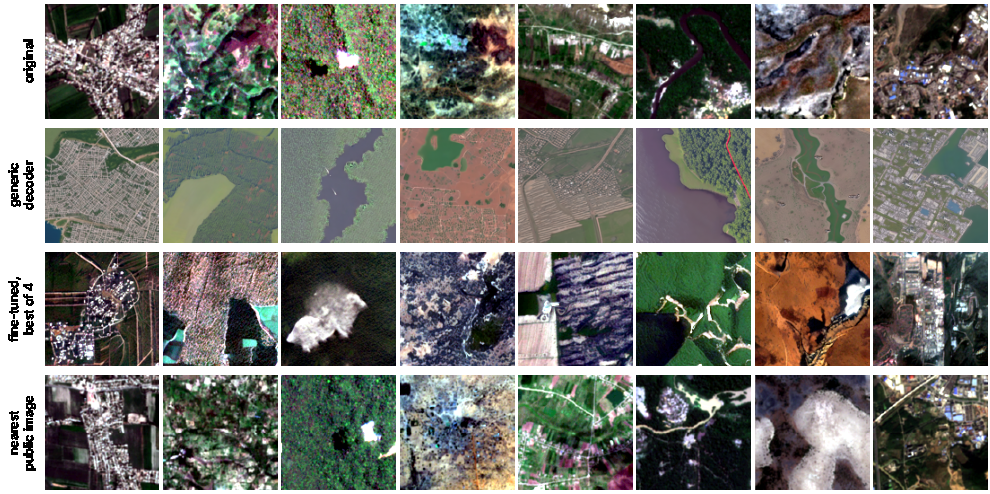
\includegraphics[width=\linewidth]{gen/fig_generic_ft.pdf}
\caption{The first eight attacked VertiBench test images (contrast-stretched for display, as the two bottom rows), the output of the generic decoder of Fig.~\ref{fig:generic}, the best of \giftNBest{} samples of the same decoder fine-tuned on public in-domain pairs, and the public image nearest to the upload in CLIP-L space, which is always of a training location.}\label{fig:generic-ft}
\end{figure}

\begin{figure}[tbp]
\centering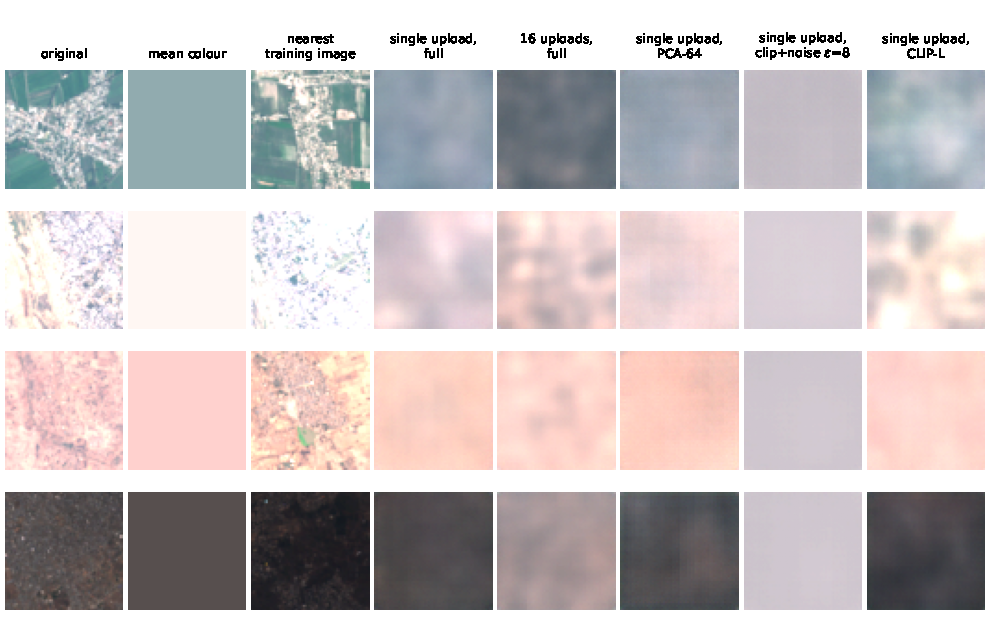
\includegraphics[width=\linewidth]{gen/fig_inversion.pdf}
\caption{Decoders trained on in-domain image--feature pairs, on held-out VertiBench test images ($64\times64$ RGB thumbnails, brightness $\times3$ for display). From left to right: original; its mean colour; nearest training image in DINOv2-g feature space; decoder output from one full DINOv2-g upload, from a PCA-64 upload, from a clipped noisy upload, and from one CLIP-L upload.}\label{fig:inversion}
\end{figure}

\begin{table}[tbp]
\caption{Utility versus leakage of the upload format on VertiBench (DINOv2-g, 224\,px). Accuracy on the test set (5 seeds); PSNR and SSIM of the single-upload inversion; re-identification (top-1, $16\times16$ thumbnails) of the source among the 12{,}560 test images and of its location among the \invNLoc{} test locations. Each value is that of the strongest attacker: the deconvolutional decoder trained for \invEpochs{} epochs, the same trained for \invShortEpochs{} epochs ($^{s}$) or the linear decoder ($^{\ell}$). Clip + noise: per-party Gaussian mechanism, per-upload $(\varepsilon, 10^{-5})$.}\label{tab:privacy}
\centering\scriptsize
\setlength{\tabcolsep}{3.5pt}
\begin{adjustbox}{max width=\linewidth}
\begin{tabular}{@{}lrccccc@{}}
\toprule
 & & & & & \multicolumn{2}{c@{}}{Re-id (\%)}\\\cmidrule(l){6-7}
Upload format & Upload & Acc. (\%) & PSNR (dB) & SSIM & image & location\\
\midrule
\inputtab{gen/tab_privacy.tex}
\bottomrule
\end{tabular}
\end{adjustbox}
\end{table}

\begin{table}[tbp]
\caption{Party-side transforms of the CLIP-L upload on VertiBench. Accuracy of the usual head on the 16 transformed uploads (3 seeds). Linkage: share of the \giVbNTest{} test uploads of a party whose embedding, mapped back to CLIP space from $k$ leaked image--upload pairs of that party ($k=0$: spectral alignment with public in-domain features), is closer to the true CLIP embedding of its image than to that of any other test image (chance \giVbChance\,\%). Raw uploads need no map: the public projection gives the embedding itself.}\label{tab:defences}
\centering\scriptsize
\setlength{\tabcolsep}{4pt}
\begin{tabular}{@{}lrcccccc@{}}
\toprule
& & & \multicolumn{5}{c@{}}{Linkage (\%) with $k$ leaked pairs}\\\cmidrule(l){4-8}
Transform & Dim. & Acc. (\%) & 0 & 10 & 100 & 1{,}000 & 3{,}142\\
\midrule
\inputtab{gen/tab_defences.tex}
\bottomrule
\end{tabular}
\end{table}

\FloatBarrier

\section{Reproducibility}\label{app:repro}

This appendix lists the code, data, compute and training details behind every result of the paper.

\paragraph{Code, data and compute.}
All code, configurations, raw result files and the scripts that generate every table, figure and quoted number from them are in the accompanying repository\footnote{\url{https://github.com/xavierxav/Simple-VFL}, directories \texttt{paper\_experiments} and \texttt{paper\_results}.}. All data sets are public. Each frozen head trains in seconds to minutes on one GPU; the whole study, including the end-to-end baselines, the image augmentation and the WorldStrat feature extraction, used about 110 Google Colab compute units on L4 and A100 GPUs.

\paragraph{Encoders and features.}
All encoders are used through their pooled output token at their native 224\,px input: DINOv2 ViT-S/B/L/g~\cite{oquab2024dinov2}, CLIP ViT-B/16 and ViT-L/14~\cite{radford2021clip}, SigLIP ViT-B/16~\cite{zhai2023siglip}, a supervised ImageNet ResNet-50 and a randomly initialised ViT-B; SSL4EO-S12 ViT-S/16~\cite{wang2023ssl4eo} on all 13 Sentinel-2 bands; BiomedCLIP~\cite{zhang2023biomedclip} and MONET~\cite{kim2024monet} for MILK10k. Satellite images are standardised per band with statistics of the released data (on WorldStrat, estimated on 200 random areas of all folds, without labels) and fed as RGB or as false-colour composites (B8-B4-B3, B12-B8A-B4) to expose the infrared bands to RGB encoders; the SPOT image is encoded at its own pixel count (1050, 518, 266 and 168\,px for 1.5, 3, 6 and 10\,m). Natural images use each model's own normalisation. Features are extracted once in half precision; a party holding several images of an entity (revisits, views) averages their features.

\paragraph{Heads.}
The reference head is a two-layer MLP ($Kd\to1000\to C$, batch normalisation, ReLU; 24.6\,M weights for 16 DINOv2-g parties, 3.1\,M for two). \emph{Late fusion} trains one MLP per party and averages their log-probabilities with a weight $w$ (chosen on the validation fold, or fixed to $\tfrac12$). A \emph{branch} head projects each party to 512 dimensions (linear, LayerNorm, GELU), classifies their concatenation, adds one auxiliary classifier per party (loss weight $\tfrac12$) and, with modality dropout, zeroes one random party in 30\,\% of the training samples. A \emph{pooling} head normalises each party's vector (LayerNorm), averages them over the parties present and applies the MLP; it requires all parties to share an encoder and feature space. A \emph{set} head applies one weight-shared MLP to each of the vectors of a party that holds several images and pools them by attention before the classifier. All heads on frozen features use Adam (learning rate $10^{-3}$, batch 512), at most 50 epochs, \texttt{ReduceLROnPlateau} and early stopping on the unweighted validation loss; the best validation checkpoint is tested (Table~\ref{tab:milkreg} checks two other stopping rules). On the imbalanced WorldStrat and MILK10k labels the loss is class-balanced and macro F1 is the primary metric.

\paragraph{Seeds, folds and tests.}
On VertiBench the public split is used as is (3{,}142 training and 785 test samples); 15\,\% of the training samples are held out for validation with the seed, so seeds change the initialisation and the validation subset, not the test set. We report mean\,$\pm$\,sample standard deviation over five seeds (VertiBench, unless noted), three seeds (CIFAR, ModelNet40; five for the protocol of Sun et al.) or five stratified cross-validation folds (WorldStrat, grouped by site; MILK10k, over lesions), where fold $f$ is the test set and fold $f{+}1$ the validation set. On the fixed VertiBench test set, comparisons use paired bootstrap intervals and exact McNemar tests on test predictions from seed-averaged probabilities (App.~\ref{app:audit}); WorldStrat and MILK10k comparisons are paired by fold. On MILK10k, the age imputation and standardisation of the metadata party are computed on all lesions, without labels.

\paragraph{Baselines.}
\emph{VertiBench recipe}: our re-implementation of the published SplitNN configuration (one ResNet-18 per party with a $9\times9$ stride-2 input convolution, MLP aggregation, Adam with learning rate $10^{-5}$, step decay, batch 32, 50 epochs, last epoch tested, 16 bottoms run sequentially) on the 13 bands. \emph{SplitNN, our recipe}: standard ResNet-18 bottoms~\cite{he2016resnet}, from scratch or ImageNet weights, and the same MLP top model as our head (Adam, one-cycle schedule, 40 epochs, batch 64, flips, best validation checkpoint). \emph{FedOnce}~\cite{wu2022fedonce}: every party trains a ResNet-18 on its unlabelled training images with Noise As Targets~\cite{bojanowski2017nat} (64-d targets, Hungarian re-assignment every 3 epochs, 100 epochs) or SimCLR~\cite{chen2020simclr} and uploads its output once; each party's encoder is pre-trained once and the five seeds re-train the head only, so the standard deviation of these rows is conditional on that pre-training. \emph{Same-backbone split learning}: frozen and LoRA-adapted CLIP ViT-B/16 bottoms on VertiBench; frozen, LoRA-adapted and (for DINOv2) fully fine-tuned CLIP ViT-B/16 and DINOv2 ViT-B/14 bottoms on MILK10k, with ResNet-18 baselines from scratch and from ImageNet weights. LoRA~\cite{hu2022lora} uses rank 16 on the attention query and value projections; the ViT runs use 10 epochs, augmentation and the best validation checkpoint, with a class-balanced loss on MILK10k. These baselines follow published or standard recipes without extensive hyper-parameter search.
